\documentclass[12pt,a4paper,twoside,openright]{book}
\usepackage[utf8]{inputenc}
\usepackage[T1]{fontenc}
\usepackage[spanish,es-tabla,es-nodecimaldot]{babel}
\usepackage[
    vmargin=2.5cm,
    headheight=15.5pt, % as per the warning by fancyhdr,
    % heightrounded, % to avoid spurious underfull messages
    includehead,
    includefoot
]{geometry}
\usepackage{graphicx}
\usepackage{amssymb}
\usepackage{amsmath}
\usepackage{fancyhdr} % create fancy headers
\usepackage{datetime2} % commands for managing dates and its formats
\usepackage[round,authoryear,sort]{natbib}
\usepackage{doi} % show dois as links on references
\usepackage{mathpazo} % Use the Palatino font by default
\usepackage[Glenn]{fncychap}  % create fancy chapter titles

% Import enumitem to customize descriptions in license.tex
\usepackage{enumitem}

% Import package to generate algorithms
\usepackage[longend,linesnumbered,ruled,spanish,onelanguage]{algorithm2e}

% Import acronym style for creating hyperref acronym and a list of acronyms
\usepackage{acronym}

% Make caption titles bold
\usepackage[labelfont=bf]{caption}

% Add toc to the toc
\usepackage{tocbibind}

% Import packages useful for creating the parameters tables
\usepackage{multirow}
\usepackage{booktabs}

% Use the appendix package and translate it
\usepackage{appendix}

% Use custom apalike bibliography style:
%   - translated to Spanish
%   - adds dois as links
\bibliographystyle{apalike-doi}

% Change margins at each side of the page
\addtolength{\oddsidemargin}{1cm}
\addtolength{\evensidemargin}{-1cm}

% Change spacing between rows in tables
\renewcommand{\arraystretch}{1.4}

% Import variables
% Title, authors and affiliations
\newcommand{\Title}{TITLE}
\newcommand{\Soler}{Santiago Rubén Soler}
\newcommand{\LicSoler}{Lic. Santiago Rubén Soler}
\newcommand{\SolerShort}{S.R. Soler}
\newcommand{\SolerMail}{santiago.r.soler@gmail.com}
\newcommand{\Mario}{Dr. Mario E. Giménez}
\newcommand{\Leo}{Dr. Leonardo Uieda}
\newcommand{\CONICET}{%
    CONICET, Argentina
}
\newcommand{\IGSV}{%
    Instituto Geofísico Sismológico Volponi, Universidad Nacional de San Juan, Argentina
}

\newcommand{\ThesisVersion}{0.1}

\newdate{publication}{\the\day}{\the\month}{\the\year}

% DOIs
\newcommand{\ThesisDOI}{XX.XXXXX/XXXXXX}

% Define inverse symbol with shorter minus
\newcommand{\inv}{^{\text{-}1}}
\newcommand{\trans}{^{\text{T}}}

% Define some units
\newcommand{\m}{$\,$m}
\newcommand{\km}{$\,$km}
\newcommand{\mGal}{$\,$mGal}


% Configure hyperref and add PDF metadata
\usepackage{hyperref}
\hypersetup{
    colorlinks,
    allcolors=[rgb]{0, 0.451, 0.753},
    pdftitle={\Title},
    pdfauthor={\Soler},
    pdfsubject={\PDFSubject},
    pdfkeywords={\PDFKeywords},
    pdftex,
}
\urlstyle{same} % make urls use the same font as every other text


% Configure headers and footers
% -----------------------------
% Configure every page of the thesis with a fancy style
\pagestyle{fancy}

% Define a command for configuring headers and footers of frontmatter
\newcommand{\fancyfront}{%
    \fancyhf{} % clear all header and footer fields
    \fancyfoot[C]{\thepage}
    \renewcommand{\headrulewidth}{0pt}
    \renewcommand{\footrulewidth}{0pt}

    % Override headers and footers for chapter pages
    \fancypagestyle{plain}{%
        \fancyhf{} % clear all header and footer fields
        \fancyfoot[C]{\thepage}
        \renewcommand{\headrulewidth}{0pt}
        \renewcommand{\footrulewidth}{0pt}
    }
}

% Define a command for configuring headers and footers of mainmatter
\newcommand{\fancymain}{%
    \fancyhf{} % clear all header and footer fields
    \fancyhead[RO,LE]{\thepage}
    \fancyhead[RE]{\leftmark}
    \fancyhead[LO]{\nouppercase{\rightmark}}
    \renewcommand{\headrulewidth}{0.4pt}

    % Override headers and footers for chapter pages
    \fancypagestyle{plain}{%
        \fancyhf{} % clear all header and footer fields
        \renewcommand{\headrulewidth}{0pt}
        \renewcommand{\footrulewidth}{0pt}
    }

}

% Clear headers and footers on blank pages before new chapter
\makeatletter
\def\cleardoublepage{
    \clearpage
    \if@twoside
        \ifodd\c@page
        \else\hbox{}\thispagestyle{empty}\newpage
            \if@twocolumn\hbox{}\newpage
            \fi
        \fi
    \fi
}
\makeatother

% Source: https://tug.org/pracjourn/2008-1/mori/mori.pdf


% =============================================================================

\begin{document}

\frontmatter
\fancyfront

\begin{titlepage}

    \begin{center}

        
\includegraphics[height=4cm]{figs/logos/unsj.pdf}
        \vspace{1.5em}

        {\Large
        UNIVERSIDAD NACIONAL DE SAN JUAN \\
        FACULTAD DE CIENCIAS EXACTAS, FÍSICAS Y NATURALES \\
        INSTITUTO GEOFÍSICO SISMOLÓGICO VOLPONI \\
        }
        \vspace{3em}

        \textbf{\LARGE TESIS DOCTORAL}
        \vspace{3em}

        \textbf{\Huge \Title}

        \vspace{\fill}

        \textbf{\LARGE Autor}
        \vspace{1em}

        {\LARGE \LicSoler{}}
        \vspace{1em}

        \rule{\linewidth}{1px}
        \vspace{1em}

        \begin{minipage}{0.45\linewidth}
            \raggedright
            \textbf{\LARGE Director}
            \vspace{1em}

            {\LARGE \Mario{}}
        \end{minipage}
        \begin{minipage}{0.45\linewidth}
            \raggedleft
            \textbf{\LARGE Codirector}
            \vspace{1em}

            {\LARGE \Leo{}}
        \end{minipage}

        \vspace{4em}

        {\Large\DTMfetchyear{publication}}

    \end{center}

\end{titlepage}


\vspace*{\fill}

\noindent \textit{\Title{}} \\
por \Soler{}

\noindent doi: \href{https://doi.org/\ThesisDOI}{\ThesisDOI}

\vspace{4em}

\noindent Versión \ThesisVersion{} \\
Última modificación el \DTMusedate{publication}.

\vspace{5em}

\noindent \includegraphics[height=2em]{figs/logos/cc-by.png}

\noindent Disponible bajo
{\bf Licencia Creative Commons Atribución 4.0 Internacional}.

\noindent
\url{https://creativecommons.org/licenses/by/4.0/deed.es}

\vspace{1em}

\noindent
Usted es libre de:

\begin{description}[labelindent=0.5cm]
    \item[Compartir:]{
        Copiar y redistribuir el material en cualquier medio o formato.
    }
    \item[Adaptar:]{
        Remezclar, transformar y construir a partir del material
        para cualquier propósito, incluso comercialmente.
    }
\end{description}

\noindent Bajo los siguientes términos:

\begin{description}[labelindent=0.5cm]
    \item[Atribución:]{
        Usted debe dar crédito de manera adecuada, brindar un enlace a la
        licencia, e indicar si se han realizado cambios. Puede hacerlo en cualquier
        forma razonable, pero no de forma tal que sugiera que usted o su uso tienen el
        apoyo del licenciante.
    }
    \item[No hay restricciones adicionales:]{
        No puede aplicar términos legales ni medidas tecnológicas que
        restrinjan legalmente a otras a hacer cualquier uso permitido por la
        licencia.
    }
\end{description}


\chapter{Agradecimientos}

% tesseroids
Nos encontramos eternamente agradecidos con los y las desarrolladores del
software open-source, sin el cual este trabajo no hubiera sido posible.
Agradecemos también al editor Kosuke Heki y a dos revisores anónimos por sus
comentarios y contribuciones.

% eqls
Nos encontramos eternamente agradecidos con los y las desarrolladores del
software open-source, sin el cual este trabajo no hubiera sido posible.
Agradecemos también al editor Frederik Simons, editor asistente Fern Storey,
y a dos revisores anónimos por sus comentarios y contribuciones.
Este trabajo contiene material de British Geological Survey ©~UKRI.


% Indice y lista de abreviaturas
\tableofcontents

\chapter{Lista de Abreviaturas}
\begin{acronym}
   \acro{GLQ}{Cuadratura de Gauss-Legendre}
   \acro{RMSE}{raíz del error cuadrático medio}
\end{acronym}


\mainmatter
\fancymain

\chapter{Introducción}

\section{Organización de la Tesis}


\chapter{Fundamentos Geofísicos}
\label{cha:fundamentos}

\section{Potencial gravitatorio}

Según la Ley de Gravitación Universal de Newton, una masa puntual $m_p$ situada
en la posición $\mathbf{p}$ se ve sometida una fuerza gravitatoria $\mathbf{F}$
debido a la presencia de otra masa $m$ situada en la posición $\mathbf{q}$.
Esta fuerza puede expresarse como:
%
\begin{equation}
    \mathbf{F} =
        - G
        \frac{m_p m}{\left\lVert \mathbf{p} - \mathbf{q}\right\rVert^3}
        (\mathbf{p} - \mathbf{q}),
\end{equation}
%
donde $G = 6.67430 \times 10^{-11} \text{m}^3 \text{kg}^{-1} \text{s}^{-2}$ es
la constante de gravitación universal y $\left\lVert \cdot \right\rVert$
representa la norma L$_2$ (Fig.~\ref{fig:potencial-gravitatorio}a).
Aplicando la segunda Ley de Newton, se deduce que la masa $m_p$ experimenta una
aceleración gravitatoria $\mathbf{g}$:
%
\begin{equation}
    \mathbf{g} =
        - \frac{G m}{\left\lVert \mathbf{p} - \mathbf{q} \right\rVert^3}
        (\mathbf{p} - \mathbf{q}).
    \label{eq:aceleracion-newton}
\end{equation}

Si consideramos que la partícula $m_p$ es una \emph{partícula de prueba},
podemos reescribir la ecuación \ref{eq:aceleracion-newton}, pero ahora
resignificándola como la aceleración gravitatoria que sentiría cualquier
partícula localizada en un punto $\mathbf{p}$ debido a la presencia de la
partícula $m$:
%
\begin{equation}
    \mathbf{g}(\mathbf{p}) =
        - \frac{G m}{\left\lVert \mathbf{p} - \mathbf{q} \right\rVert^3}
        (\mathbf{p} - \mathbf{q}).
\end{equation}

Se puede demostrar que la atracción gravitatoria $\mathbf{g}$ define un campo
irrotacional, es decir:
%
\begin{equation}
    \nabla \times \mathbf{g} = 0.
\end{equation}
%
Por ende es posible definir un potencial escalar $V$ al que
denominaremos \emph{potencial gravitatorio}:
%
\begin{equation}
    \mathbf{g}(\mathbf{p}) = + \nabla V(\mathbf{p}),
    \label{eq:potencial-gravitatorio-definicion}
\end{equation}
%
donde
%
\begin{equation}
    V(\mathbf{p}) =
      G \frac{m}{\left\lVert \mathbf{p} - \mathbf{q} \right\rVert}.
    \label{eq:potencial-gravitatorio-particula}
\end{equation}
%
Vale la pena notar que en la ecuación
\ref{eq:potencial-gravitatorio-definicion} se ha aplicado la convención de
signo positivo para definir el potencial $V$, mayormente utilizada en la
literatura sobre Geofísica y Geodesia
\citep{heiskanen1967,blakely1995,hinze2009}.

\begin{figure}
    \centering
    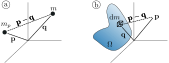
\includegraphics[width=\linewidth]{figs/gravity-potentials.pdf}
    \caption{
        (a)~Masas puntuales $m_p$ y $m$ localizadas en $\mathbf{p}$
        y $\mathbf{q}$, respectivamente.
        (b)~Distribución de masa $\Omega$, diferencial de masa $\diff m$
        ubicado en el punto $\mathbf{q}$.
    }
    \label{fig:potencial-gravitatorio}
\end{figure}


\subsection{Potencial gravitatorio por una distribución de masa}

Partiendo de que un diferencial de masa $\diff m$ ubicado en $\mathbf{q}$
genera un potencial gravitatorio $\diff V$ en cualquier punto $\mathbf{p}$
(Fig.~\ref{fig:potencial-gravitatorio}b):
%
\begin{equation}
    \diff V(\mathbf{p}) = \frac{G}{\left\lVert \mathbf{p} - \mathbf{q}
        \right\rVert} \diff m,
\end{equation}
%
el potencial gravitatorio generado por una distribución de masa
$\Omega$ puede calcularse integrando los diferenciales de masa que lo componen:
%
\begin{equation}
    V(\mathbf{p}) =
        G \int\limits_\Omega \frac{\diff m}{\left\lVert \mathbf{p} - \mathbf{q}
            \right\rVert} .
\end{equation}

Si reescribimos los diferenciales de masa como
%
\begin{equation}
    \diff m = \rho(\mathbf{q}) \diff v,
\end{equation}
%
donde $\rho(\mathbf{q})$ es la densidad de masa de la distribución
$\Omega$ en el punto $\mathbf{q}$ y $\diff v$ es el diferencial de volumen,
el potencial se puede expresar como:
%
\begin{equation}
    V(\mathbf{p}) =
        G \int\limits_\Omega
        \frac{\rho(\mathbf{q})}{\left\lVert \mathbf{p} - \mathbf{q}
            \right\rVert} \diff v.
    \label{eq:potencial-gravitatorio-integral}
\end{equation}


\subsection{Gradiente del potencial gravitatorio}

Según la definición del potencial gravitatorio expuesta en la
ecuación~\ref{eq:potencial-gravitatorio-definicion}, es posible calcular la
aceleración de la gravedad producida por una distribución de masa arbitraria
en cualquier punto $\mathbf{p}$ como el gradiente del potencial
$V(\mathbf{p})$.
Si definimos un sistema de ejes Cartesianos en el cual el punto
$\mathbf{p} = (x, y, z)$, las componentes de la aceleración en cada una de las
direcciones del sistema quedan expresadas como:
%
\begin{equation}
    g_i(\mathbf{p}) = \frac{\partial V(\mathbf{p})}{\partial i}, \,\,
        \forall i \in \{x, y, z\}.
    \label{eq:componentes-aceleracion-gravitatoria}
\end{equation}

El vector
$\mathbf{g}(\mathbf{p}) = (g_x(\mathbf{p}), g_y(\mathbf{p}), g_z(\mathbf{p}))$
representa la aceleración gravitatoria en el punto
$\mathbf{p}$ generada por la distribución de masa $\Omega$, aunque es común
referirse al mismo como el \emph{gradiente gravitatorio}.
Reemplazando la ecuación~\ref{eq:potencial-gravitatorio-integral}
en~\ref{eq:componentes-aceleracion-gravitatoria}, las componentes del gradiente
gravitatorio pueden expresarse como:
%
\begin{align}
    g_x(\mathbf{p}) &=
        - G \int\limits_\Omega \rho(\mathbf{q})
        \frac{(x - x')}{\left\lVert \mathbf{p} - \mathbf{q} \right\rVert^3}
        \diff v,
    \label{eq:gx-integral}
    \\
    g_y(\mathbf{p}) &=
        - G \int\limits_\Omega \rho(\mathbf{q})
        \frac{(y - y')}{\left\lVert \mathbf{p} - \mathbf{q} \right\rVert^3}
        \diff v,
    \label{eq:gy-integral}
    \\
    g_z(\mathbf{p}) &=
        - G \int\limits_\Omega \rho(\mathbf{q})
        \frac{(z - z')}{\left\lVert \mathbf{p} - \mathbf{q} \right\rVert^3}
        \diff v,
    \label{eq:gz-integral}
\end{align}
%
donde $\mathbf{q} = (x', y', z')$.

Las segundas derivadas del potencial gravitatorio definen el \emph{tensor del
gradiente gravitatorio}, y sus componentes pueden expresarse como:
%
\begin{equation}
    g_{ij}(\mathbf{p}) =
        \frac{\partial^2 V(\mathbf{p})}{\partial i \partial j}, \,\,
        \forall i \in \{x, y, z\}, \,\,
        \forall j \in \{x, y, z\}.
\end{equation}

Reemplazando la ecuación \ref{eq:potencial-gravitatorio-integral}, podemos
expresar las componentes diagonales del tensor de la siguiente manera
\citep{grombein2013}:
%
\begin{align}
    g_{xx}(\mathbf{p}) &=
        G \int\limits_\Omega \rho(\mathbf{q})
        \left[
        \frac{3(x - x')^2}{\left\lVert \mathbf{p} - \mathbf{q} \right\rVert^5}
        - \frac{1}{\left\lVert \mathbf{p} - \mathbf{q} \right\rVert^3}
        \right]
        \diff v,
    \label{eq:gxx-integral}
    \\
    g_{yy}(\mathbf{p}) &=
        G \int\limits_\Omega \rho(\mathbf{q})
        \left[
        \frac{3(y - y')^2}{\left\lVert \mathbf{p} - \mathbf{q} \right\rVert^5}
        - \frac{1}{\left\lVert \mathbf{p} - \mathbf{q} \right\rVert^3}
        \right]
        \diff v,
    \label{eq:gyy-integral}
    \\
    g_{zz}(\mathbf{p}) &=
        G \int\limits_\Omega \rho(\mathbf{q})
        \left[
        \frac{3(z - z')^2}{\left\lVert \mathbf{p} - \mathbf{q} \right\rVert^5}
        - \frac{1}{\left\lVert \mathbf{p} - \mathbf{q} \right\rVert^3}
        \right]
        \diff v,
    \label{eq:gzz-integral}
\end{align}
%
mientras que las componentes no diagonales pueden expresarse como:
%
\begin{align}
    g_{xy}(\mathbf{p}) =
    g_{yx}(\mathbf{p}) &=
        G \int\limits_\Omega \rho(\mathbf{q})
        \frac{
            3(x - x')(y - y')
        }{
            \left\lVert \mathbf{p} - \mathbf{q} \right\rVert^5
        }
        \diff v,
    \label{eq:gxy-integral}
    \\
    g_{xz}(\mathbf{p}) =
    g_{zx}(\mathbf{p}) &=
        G \int\limits_\Omega \rho(\mathbf{q})
        \frac{
            3(x - x')(z - z')
        }{
            \left\lVert \mathbf{p} - \mathbf{q} \right\rVert^5
        }
        \diff v,
    \label{eq:gxz-integral}
    \\
    g_{yz}(\mathbf{p}) =
    g_{zy}(\mathbf{p}) &=
        G \int\limits_\Omega \rho(\mathbf{q})
        \frac{
            3(y - y')(z - z')
        }{
            \left\lVert \mathbf{p} - \mathbf{q} \right\rVert^5
        }
        \diff v.
    \label{eq:gyz-integral}
\end{align}

A partir de las ecuaciones~\ref{eq:gxx-integral}--\ref{eq:gzz-integral} podemos
calcular el Laplaciano del potencial gravitatorio:
%
\begin{equation}
    \nabla^2 V(\mathbf{p}) =
        \frac{\partial^2 V}{\partial x^2}
        + \frac{\partial^2 V}{\partial y^2}
        + \frac{\partial^2 V}{\partial z^2},
\end{equation}
%
Dado que las tres expresiones se cancelan mutuamente
\citep{blakely1995}, podemos concluir que cualquier potencial gravitatorio es
un \emph{campo armónico}
%
\begin{equation}
    \nabla^2 V(\mathbf{p}) = 0
    \label{eq:potencial-laplace}
\end{equation}
%
para cualquier punto de observación $\mathbf{p}$ fuera de la
distribución de masa $\Omega$.

Vale notar que la ecuación de Laplace \ref{eq:potencial-laplace} es válida
solo para regiones libres de masas, y representa un caso particular de la
ecuación de Poisson \citep{blakely1995}:
%
\begin{equation}
    \nabla^2 V(\mathbf{p}) = -4\pi G \, \rho(\mathbf{p}),
    \label{eq:potencial-poisson}
\end{equation}
%
válida para cualquier punto de observación $\mathbf{p}$.

% =============================================================================

\section{Modelado directo}

El cálculo de los efectos gravitatorios de un determinado cuerpo sobre uno
o más puntos de observación se suele denominar modelado directo (\emph{forward
modelling} en inglés).
Aunque las expresiones del potencial gravitatorio
(ec.~\ref{eq:potencial-gravitatorio-integral}),
las componentes de su gradiente
(ecs.~\ref{eq:gx-integral}--\ref{eq:gz-integral})
y de su tensor (ecs.~\ref{eq:gxx-integral}--\ref{eq:gzz-integral})
aparentan ser sencillas, el cómputo de estas magnitudes para una geometría dada
no resulta un problema trivial.
Solo existen soluciones analíticas a dichas expresiones para determinadas
geometrías sencillas o que guardan algún tipo de simetría.

En el desarrollo de esta Tesis nos resultan de principal interés trabajar con
tres tipos de geometrías: masas puntuales, prismas rectangulares y prismas
esféricos o \emph{teseroides}.

\subsection{Masas puntuales}

La distribución de densidades de una masa puntual puede expresarse
sencillamente mediante una Delta de Dirac \citep{vladimirov1979}:
%
\begin{equation}
    \rho(\mathbf{q}) = m \, \delta(\mathbf{q} - \mathbf{q'}),
\end{equation}
%
donde $\mathbf{q}$ y $m$ son la posición y la masa de la partícula,
respectivamente.
Reemplazando esta expresión en la
ecuación~\ref{eq:potencial-gravitatorio-integral}, obtenemos el potencial
gravitatorio generado por una partícula:
%
\begin{equation}
    V(\mathbf{p}) =
        G \int\limits_\Omega
        m \frac{\delta(\mathbf{q} - \mathbf{q'})}{\left\lVert \mathbf{p}
            - \mathbf{q'} \right\rVert}
        \diff v =
        \frac{G m}{\left\lVert \mathbf{p} - \mathbf{q} \right\rVert},
    \label{eq:potencial-masa-puntual}
\end{equation}
%
de acuerdo con la expresión del potencial de la
ecuación~\ref{eq:potencial-gravitatorio-particula}.

Realizando el mismo reemplazo en las ecuaciones correspondientes a las
componentes del gradiente (ecs.~\ref{eq:gx-integral}--\ref{eq:gz-integral})
arribamos a las siguientes expresiones:
%
\begin{align}
    g_x(\mathbf{p}) &=
        - G m
        \frac{x - x'}{\left\lVert \mathbf{p} - \mathbf{q} \right\rVert^3},
    \label{eq:gx-particula}
    \\
    g_y(\mathbf{p}) &=
        - G m
        \frac{y - y'}{\left\lVert \mathbf{p} - \mathbf{q} \right\rVert^3},
    \label{eq:gy-particula}
    \\
    g_z(\mathbf{p}) &=
        - G m
        \frac{z - z'}{\left\lVert \mathbf{p} - \mathbf{q} \right\rVert^3}.
    \label{eq:gz-particula}
\end{align}

A la hora de realizar el cómputo de los campos gravitatorios de masas
puntuales, las posiciones de las partículas como de los puntos de observación
pueden venir dados en diferentes sistemas de coordenadas.
En el caso de necesitar modelar cualquier conjunto de masas situadas bajo la
superficie terrestre, resulta natural utilizar coordenadas esféricas tanto para
las posiciones de las partículas como para los puntos de observación.
Sin embargo, es muy común trabajar sobre zonas de estudio con dimensiones
acotadas, bajo las cuales la aproximación de Tierra plana es suficiente. En
estos casos es posible trabajar en coordenadas Cartesianas.

\subsubsection{Coordenadas Cartesianas}

En el caso de que la posición de la partícula venga dada por el vector
$\mathbf{q} = (x', y', z')$ y el punto de observación por el vector
$\mathbf{p} = (x, y, z)$ definidos en el mismo sistema de ejes Cartesianos, el
módulo de
$\mathbf{p} - \mathbf{q}$ se calcula sencillamente bajo la norma L$_2$:
%
\begin{equation}
    \left\lVert  \mathbf{p} - \mathbf{q}  \right\rVert = \sqrt{
        (x - x')^2 + (y - y')^2 + (z - z')^2
    }.
\end{equation}

Dado que los numeradores en las
ecuaciones~\ref{eq:gx-particula}--\ref{eq:gz-particula} resultan triviales en
coordenadas Cartesianas, el cómputo del potencial y las componentes de su
gradiente se puede realizar de manera sencilla.

\subsubsection{Coordenadas esféricas}

Consideremos que las posiciones del punto de observación y de la partícula
vienen dados en un sistema de coordenadas esféricas. Para ello vamos a definir
un sistema de referencia \emph{geocéntrico} $\{X, Y, Z\}$ y a partir del mismo
un sistema de coordenadas esféricas $\{r, \lambda, \phi\}$, donde $r$ es la
posición \emph{radial}, $\lambda$ la posición \emph{longitudinal} y $\phi$ la
posición \emph{latitudinal} (Fig.~\ref{fig:spherical-coordinates}).
Cualquier punto dado por las coordenadas esféricas $(r, \lambda, \phi)$ se
puede expresar en coordenadas Cartesianas geocéntricas bajo las siguientes
relaciones:
%
\begin{equation}
    \begin{cases}
        X = r \cos\lambda \cos{\phi} \\
        Y = r \sin\lambda \cos{\phi} \\
        Z = r \sin{\phi},
    \end{cases}
\end{equation}
%
donde $r \in [0, \infty)$, $\lambda \in (-\pi, \pi]$ y
$\phi \in [-\pi/2, \pi/2]$.

\begin{figure}[t]
    \centering
    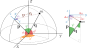
\includegraphics[width=\linewidth]{figs/spherical-coordinates.pdf}
    \caption{
        Masa puntual $m$ ubicada en la posición $\mathbf{q}$ y punto de
        observación situado en $\mathbf{p}$.
        Se define un sistema de referencia Cartesiano \emph{geocéntrico} $X, Y,
        Z$ bajo el cual se considera un sistema de coordenadas esféricas dadas
        por la distancia radial ($r$), ángulo longitudinal ($\lambda$) y ángulo
        latitudinal ($\phi$).
        En el punto $\mathbf{p}$ se define un sistema \emph{local} de
        coordenadas Cartesiano: el eje $x$ apunta hacia el Este,
        el eje $y$ hacia el Norte geométrico y el eje $z$ en la dirección
        radial.
        Se define a $\psi$ como el ángulo descripto por los vectores
        $\mathbf{p}$ y $\mathbf{q}$, y $\alpha$ al ángulo azimutal de
        $\mathbf{q} - \mathbf{p}$ sobre el sistema \emph{local}.
    }
    \label{fig:spherical-coordinates}
\end{figure}

El potencial gravitatorio que genera la partícula $m$ sobre el punto de
observación $\mathbf{p}$ puede calcularse mediante la
ecuación~\ref{eq:potencial-gravitatorio-particula}.
Considerando que los vectores $\mathbf{p}$ y $\mathbf{q}$ vienen definidos por
las coordenadas esféricas $(r, \lambda, \phi)$ y $(r', \lambda', \phi')$,
respectivamente, la distancia Euclidiana entre ellos puede expresarse como
\citep{grombein2013}:
%
\begin{equation}
    \left\lVert \mathbf{p} - \mathbf{q} \right\rVert = \sqrt{
        r^2 + r'^2 - 2rr'\cos\psi
    },
    \label{eq:distance-spherical}
\end{equation}
%
donde $\psi$ es el ángulo que describen los vectores $\mathbf{p}$
y $\mathbf{q}$:
%
\begin{equation}
    \cos \psi =
        \sin \phi \sin \phi' + \cos \phi \cos \phi' \cos(\lambda - \lambda').
    \label{eq:cosphi}
\end{equation}

La determinación de las componentes del gradiente del potencial gravitatorio
hace necesario que definamos las direcciones ortogonales $x$, $y$ y $z$ a lo
largo de las cuales se calculan las derivadas parciales de $V(\mathbf{p})$.
La elección más natural es obtener el gradiente con respecto a un sistema de
coordenadas \emph{local} $\{x, y, z\}$ \citep{grombein2013,uieda2016} donde $x$
se orienta en la dirección longitudinal (Este), $y$ en la dirección latitudinal
(Norte) y $z$ en la dirección radial.

Los numeradores de las ecuaciones~\ref{eq:gx-particula}--\ref{eq:gz-particula}
pueden expresarse en términos de las coordenadas esféricas como:
%
\begin{align}
    \Delta x &= - (x - x') = r' \sin\psi \cos\alpha
    \label{eq:delta-x-raw}
    \\
    \Delta y &= - (y - y') = r' \sin\psi \sin\alpha
    \label{eq:delta-y-raw}
    \\
    \Delta z &= - (z - z') = r'\cos\psi - r,
    \label{eq:delta-z-raw}
\end{align}
%
donde $\alpha$ es el ángulo azimutal del vector
$\mathbf{q} - \mathbf{p}$ sobre el sistema de coordenadas \emph{locales}.
Haciendo uso de las siguientes relaciones de trigonometría esférica
\citep[][p.~113]{heiskanen1967}:
%
\begin{align}
    \sin\psi \cos\alpha &=
        \cos\phi \sin\phi' - \sin\phi \cos\phi' \cos(\lambda - \lambda') \\
    \sin\psi \sin\alpha &=
        \cos\phi' \sin(\lambda - \lambda'),
\end{align}
%
podemos expresar las ecuaciones~\ref{eq:delta-x-raw},
\ref{eq:delta-y-raw} y \ref{eq:delta-z-raw} como \citep{grombein2013}:
%
\begin{align}
    \Delta x &= r' \sin\psi \left[
        \cos\phi \sin\phi' - \sin\phi \cos\phi' \cos(\lambda - \lambda')
        \right]
    \label{eq:delta-x}
    \\
    \Delta y &= r' \cos\phi' \sin(\lambda - \lambda')
    \label{eq:delta-y}
    \\
    \Delta z &= r'\cos\psi - r.
    \label{eq:delta-z}
\end{align}

Las componentes del gradiente del potencial gravitatorio generado por una masa
puntual en coordenadas esféricas quedan determinadas de la siguiente manera:
%
\begin{align}
    g_x(\mathbf{p}) &=
        G m
        \frac{\Delta x}{\left\lVert \mathbf{p} - \mathbf{q} \right\rVert^3},
    \label{eq:gx-particula-spherical}
    \\
    g_y(\mathbf{p}) &=
        G m
        \frac{\Delta y}{\left\lVert \mathbf{p} - \mathbf{q} \right\rVert^3},
    \label{eq:gy-particula-spherical}
    \\
    g_z(\mathbf{p}) &=
        G m
        \frac{\Delta z}{\left\lVert \mathbf{p} - \mathbf{q} \right\rVert^3},
    \label{eq:gz-particula-spherical}
\end{align}
%
haciendo uso de las ecuaciones~\ref{eq:distance-spherical},
\ref{eq:cosphi}, \ref{eq:delta-x}, \ref{eq:delta-y} y \ref{eq:delta-z}.


\subsection{Prismas rectangulares}
\label{sec:prismas-rectangulares}

A la hora de modelar estructuras tridimensionales subyacentes a la superficie
terrestre, los primas rectangulares se presentan como la geometría a elección
por parte de muchos autores y muchas autoras.
Una de las razones recae en la simpleza de la geometría, que resulta muy útil
para modelar estructuras geológicas.
Aunque quizás la principal razón es la existencia de soluciones analíticas
a las ecuaciones de los campos gravitatorios generados por prismas
rectangulares \citep{nagy2000,nagy2002}.

Consideremos un prisma rectangular de densidad homogénea $\rho$ cuyos vértices
se encuentran determinados por las coordenadas $X_1, X_2, Y_1, Y_2, Z_1, Z_2$
definidas en un sistema de ejes Cartesianos ${X, Y, Z}$
(Fig.~\ref{fig:rectangular-prism}).
El potencial gravitatorio que genera el prisma sobre un punto de observación
$\mathbf{p} = (X, Y, Z)$ definido en el sistema ${X, Y, Z}$ se puede
calcular mediante la ecuación~\ref{eq:potencial-gravitatorio-integral},
reemplazando el dominio de integración:
%
\begin{equation}
    V(\mathbf{p}) =
    G \rho
    \int\limits_{X_1}^{X_2}
    \int\limits_{Y_1}^{Y_2}
    \int\limits_{Z_1}^{Z_2}
    \frac{\diff X' \diff Y' \diff Z'}{\left\lVert \mathbf{p} - \mathbf{q}
        \right\rVert},
\end{equation}
%
donde
%
\begin{equation}
    \left\lVert \mathbf{p} - \mathbf{q} \right\rVert = \sqrt{
        (X - X')^2 + (Y - Y')^2 + (Z - Z')^2
    }.
\end{equation}

\begin{figure}[t]
    \centering
    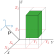
\includegraphics[width=0.6\linewidth]{figs/rectangular-prism.pdf}
    \caption{
        Prisma rectangular y punto de observación $\mathbf{p}$ definidos en un
        sistema de coordenadas Cartesianas $\{X, Y, Z\}$. Se define un sistema
        de coordenadas Cartesianas $\{x, y, z\}$ con origen en el punto de
        observación $\mathbf{p}$ y con ejes paralelos a $X, Y, Z$,
        respectivamente.
    }
    \label{fig:rectangular-prism}
\end{figure}

Con el objetivo de simplificar los cálculos, definimos un sistema de
coordenadas Cartesianas $\{x, y, z\}$ cuyo origen se encuentra en el punto de
observación $\mathbf{p}$ y sus ejes son paralelos a los del sistema $\{X, Y,
Z\}$, respectivamente (Fig.~\ref{fig:rectangular-prism}).
Los vértices del prisma vendrán dados por las coordenadas
$x_1, x_2, y_1, y_2, z_1, z_2$ en el nuevo sistema de referencia, es decir:
%
\begin{equation}
    \begin{aligned}
        x_1 &= X_1 - X, & x_2 &= X_2 - X, \\
        y_1 &= Y_1 - Y, & y_2 &= Y_2 - Y, \\
        z_1 &= Z_1 - Z, & z_2 &= Z_2 - Z.
    \end{aligned}
\end{equation}

Bajo este nuevo sistema de referencia, el potencial gravitatorio se puede
expresar como:
%
\begin{equation}
    V(\mathbf{p}) =
    G \rho
    \int\limits_{x_1}^{x_2}
    \int\limits_{y_1}^{y_2}
    \int\limits_{z_1}^{z_2}
    \frac{\diff x' \diff y' \diff z'}{\sqrt{{x'}^2 + {y'}^2 + {z'}^2}}.
\end{equation}

El resultado de esta integración posee la siguiente forma
\citep{nagy2000,nagy2002}:
%
\begin{equation}
    \begin{split}
        V(\mathbf{p}) =
        G \rho
        \Bigg[ &
            xy \ln (z + l) + yz \ln(x + l) + zx \ln(y + l) \\
               &
            - \frac{x^2}{2} \arctan \frac{yz}{xl}
            - \frac{y^2}{2} \arctan \frac{zx}{yl}
            - \frac{z^2}{2} \arctan \frac{xy}{zl}
        \Bigg]
        \Bigg|_{x_1}^{x_2}
        \Bigg|_{y_1}^{y_2}
        \Bigg|_{z_1}^{z_2},
    \end{split}
    \label{eq:potencial-prismas-analitico}
\end{equation}
%
donde
%
\begin{equation}
    l = \sqrt{x^2 + y^2 + z^2}.
\end{equation}

Reemplazando todos los límites del dominio de integración, obtenemos un total
de 48 términos.
A la hora de evaluarlos numéricamente hay que tener en cuenta que la solución
analítica de la ecuación~\ref{eq:potencial-prismas-analitico} no es
continua en todo $\mathbb{R}^3$, particularmente en los casos en los que el
punto de observación se encuentra sobre alguno de los vértices, aristas o caras
del prisma ($x_{1,2}=0$, $y_{1,2}=0$ ó $z_{1,2}=0$). Sin embargo el potencial
$V(\mathbf{p})$ sí lo es.
Para solucionar esto, es necesario reemplazar aquellos términos que no pueden
ser evaluados por sus límites cuando $(x, y, z) \rightarrow (0, 0, 0)$
\citep{nagy2000}.
Por ejemplo:
%
\begin{equation}
    \lim_{(x, y, z)\rightarrow (0, 0, 0)} xz \ln(z + r) = 0.
\end{equation}

Una solución alternativa es reemplazar la función $\ln$ por una nueva función
$\safelog(x)$ definida de la siguiente manera:
%
\begin{equation}
    \safelog(x) =
    \begin{cases}
        \ln(x) & \quad x \ge x_\text{umbral} \\
        0      & \quad x < x_\text{umbral}
    \end{cases}
    \label{eq:safe_log}
\end{equation}
%
donde $x_\text{umbral}$ es un valor muy pequeño del argumento de
$\safelog$ a partir del cual consideramos que la función debe ser evaluada en
su límite en cero.
La elección de este valor dependerá de las dimensiones del problema que estamos
resolviendo.
En el caso de un modelado directo geofísico, en el cual las dimensiones de los
primas vienen dadas por varios metros, podemos asumir un valor de
$x_\text{umbral} = 10^{-10}$m \citep{harmonica2021}.

Por otro lado, la evaluación de la función $\arctan$ requiere ciertos cuidados.
Para que el potencial $V(\mathbf{p})$ satisfaga la ecuación de Poisson
(ec.~\ref{eq:potencial-poisson}), es necesario utilizar la siguiente forma de
la función $\safearctan(y, x)$ \citep{fukushima2020}:
%
\begin{equation}
    \safearctan(y, x) =
    \begin{cases}
        \arctan(y / x) & \quad x \ne 0 \\
        \pi / 2        & \quad x = 0,\, y > 0 \\
        -\pi / 2       & \quad x = 0,\, y < 0 \\
        0              & \quad x = 0,\, y = 0.
    \end{cases}
    \label{eq:safe_arctan}
\end{equation}

Haciendo uso de las funciones $\safelog$ y $\safearctan$ definidas en las
ecuaciones~\ref{eq:safe_log} y \ref{eq:safe_arctan}, respectivamente, el
potencial gravitatorio generado por un prisma rectangular en cualquier punto de
observación $\mathbf{p}$ puede ser numéricamente calculado mediante:
%
\begin{equation}
    \begin{split}
        V(\mathbf{p}) =
        G \rho
        \Bigg[ &
            xy \safelog (z + l)
            + yz \safelog(x + l)
            + zx \safelog(y + l)
           - \frac{x^2}{2} \safearctan(yz, xl)
                \\&
           - \frac{y^2}{2} \safearctan(zx, yl)
           - \frac{z^2}{2} \safearctan(xy, zl)
        \Bigg]
        \Bigg|_{x_1}^{x_2}
        \Bigg|_{y_1}^{y_2}
        \Bigg|_{z_1}^{z_2}.
    \end{split}
    \label{eq:potencial-prismas-numerico}
\end{equation}

De manera análoga, podemos calcular las componentes del gradiente del potencial
gravitatorio generado por un prisma rectangular haciendo uso de las siguientes
expresiones \citep{nagy2000,nagy2002}:
%
\begin{align}
    g_x(\mathbf{p}) =&
        \Big[
            y \safelog(z + l) + z \safelog(y + l)  - x \safearctan(yz, xl)
        \Big]
        \Big|_{x_1}^{x_2}
        \Big|_{y_1}^{y_2}
        \Big|_{z_1}^{z_2} \\
    g_y(\mathbf{p}) =&
        \Big[
            z \safelog(x + l) + x \safelog(z + l)  - y \safearctan(zx, yl)
        \Big]
        \Big|_{x_1}^{x_2}
        \Big|_{y_1}^{y_2}
        \Big|_{z_1}^{z_2} \\
    g_z(\mathbf{p}) =&
        \Big[
            x \safelog(y + l) + y \safelog(x + l) - z \safearctan(xy, zl)
        \Big]
        \Big|_{x_1}^{x_2}
        \Big|_{y_1}^{y_2}
        \Big|_{z_1}^{z_2}.
\end{align}


\subsection{Teseroides}

En caso de querer realizar modelos directos de estructuras regionales,
continentales o globales, el uso de prismas rectangulares en coordenadas
Cartesianas no resulta la mejor opción, ya que no tienen en cuenta la curvatura
del planeta Tierra.
La mayoría de los modelos directos que sí lo hacen se definen en coordenadas
esféricas geocéntricas y consisten en discretizar la Tierra en geometrías
simples.
Este es el caso de los \emph{teseroides} \citep{anderson1976}, también
conocidos como prismas esféricos, los cuales se definen como el volumen
comprendido entre dos esferas de radios distintos, dos meridianos de longitudes
distintas y dos paralelos de distintas latitudes (Fig.~\ref{fig:tesseroid}).

\begin{figure}
    \centering
    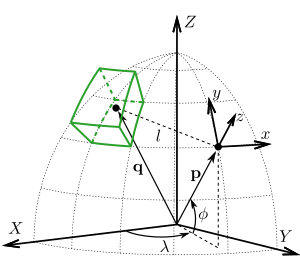
\includegraphics[width=0.7\linewidth]{figs/tesseroid-coord-sys.pdf}
    \caption{
        Teseroide (prisma esférico) en un sistema de coordenadas esféricas
        geocéntricas, junto a un punto de cómputo situado en $\mathbf{p}$ y su
        correspondiente sistema \emph{local} de coordenadas Cartesianas.
        Obtenida de \citet{uieda2015}.
    }
    \label{fig:tesseroid}
\end{figure}

El potencial gravitatorio que genera un teseroide de densidad uniforme $\rho$,
definido por las coordenadas $r_1$, $r_2$, $\lambda_1$, $\lambda_2$, $\phi_1$
y $\phi_2$, sobre un punto de observación $\mathbf{p}$, dado por las
coordenadas esféricas $r$, $\lambda$ y $\phi$, se puede obtener aplicando estos
límites de integración a la ecuación~\ref{eq:potencial-gravitatorio-integral},
quedando expresado como la siguiente integral volumétrica
\citep{grombein2013,uieda2016}:
%
\begin{equation}
    V(\mathbf{p}) = G \rho
        \int\limits_{r_1}^{r_2}
        \int\limits_{\lambda_1}^{\lambda_2}
        \int\limits_{\phi_1}^{\phi_2}
        \frac{\kappa}{\left\lVert \mathbf{p} - \mathbf{q} \right\rVert}
        \diff r' \diff \lambda' \diff \phi',
    \label{eq:potencial-teseroide}
\end{equation}
%
donde
%
\begin{equation}
    \kappa = {r'}^2 \cos \phi',
    \label{eq:kappa}
\end{equation}
%
la distancia $\left\lVert \mathbf{p} - \mathbf{q} \right\rVert$ viene
dada por la ecuación~\ref{eq:distance-spherical} y las coordenadas de
integración $r'$, $\lambda'$ y $\phi'$ representan la posición $\mathbf{q}$ de
cada volumen infinitesimal del teseroide.

Reemplazando los límites de integración de las ecuaciones \ref{eq:gx-integral},
\ref{eq:gy-integral} y \ref{eq:gz-integral} por los del teseroide, podemos
obtener las componentes del gradiente del potencial gravitatorio generado por
el teseroide en el punto de observación $\mathbf{p}$ con respecto al
sistema de coordenadas \emph{local}:
%
\begin{align}
    g_x(\mathbf{p}) &=
        G \rho
        \int\limits_{r_1}^{r_2}
        \int\limits_{\lambda_1}^{\lambda_2}
        \int\limits_{\phi_1}^{\phi_2}
        \frac{\Delta x}{\left\lVert \mathbf{p} - \mathbf{q} \right\rVert^3}
        \kappa
        \diff r' \diff \lambda' \diff \phi',
    \label{eq:gx-teseroide}
    \\
    g_y(\mathbf{p}) &=
        G \rho
        \int\limits_{r_1}^{r_2}
        \int\limits_{\lambda_1}^{\lambda_2}
        \int\limits_{\phi_1}^{\phi_2}
        \frac{\Delta y}{\left\lVert \mathbf{p} - \mathbf{q} \right\rVert^3}
        \kappa
        \diff r' \diff \lambda' \diff \phi',
    \label{eq:gy-teseroide}
    \\
    g_z(\mathbf{p}) &=
        G \rho
        \int\limits_{r_1}^{r_2}
        \int\limits_{\lambda_1}^{\lambda_2}
        \int\limits_{\phi_1}^{\phi_2}
        \frac{\Delta z}{\left\lVert \mathbf{p} - \mathbf{q} \right\rVert^3}
        \kappa
        \diff r' \diff \lambda' \diff \phi',
    \label{eq:gz-teseroide}
\end{align}
%
donde $\Delta x$, $\Delta y$ y $\Delta z$ vienen dadas por las
ecuaciones~\ref{eq:delta-x}, \ref{eq:delta-y} y \ref{eq:delta-z},
respectivamente.

Las ecuaciones~\ref{eq:potencial-teseroide}, \ref{eq:gx-teseroide},
\ref{eq:gy-teseroide} y \ref{eq:gz-teseroide} contienen integrales elípticas
que no poseen solución analítica y deben ser aproximadas numéricamente.
Existen dos principales métodos en la literatura para aproximar estas
integrales: uno involucra expansiones en serie de Taylor
\citep{heck2006,grombein2013} mientras que los otros hacen uso de la \ac{GLQ}
\citep{asgharzadeh2007,wildpfeiffer2008,li2011,uieda2016,lin2018}.
En el Capítulo~\ref{cha:tesseroids-variable-density} se detallan las razones
por las cuales a lo largo de esta Tesis abordaremos la estrategia de la
\ac{GLQ}.

La \Ac{GLQ} consiste en la aproximación de una integral por una suma ponderada
del integrando evaluado en determinadas abscisas
\citep[][p.~390]{hildebrand1987}:
%
\begin{equation}
    \int\limits_{-1}^1 f(x) \diff x \approx
        \sum\limits_{i=1}^{N} W_i f(x_i),
\end{equation}
%
donde $N$ es el orden de la cuadratura,
$x_i$ corresponden a las raíces del polinomio de Legendre $P_N(x)$ de grado
$N$, y $W_i$ son los pesos ponderados de cada término:
%
\begin{equation}
    W_i = \frac{2}{(1 - x_i^2) \Big[ P'_N(x_i) \Big]^2}.
\end{equation}
%
El polinomio de Legendre $P_N(x)$ se puede obtener mediante
relaciones de recurrencia \citep[][p.~330]{hildebrand1987}:
%
\begin{align}
    &P_0(x) = 1 \\
    &P_1(x) = x \\
    &P_{N + 1}(x) = \frac{2N + 1}{N + 1} x P_N(x) - \frac{N}{N + 1}P_{N-1}(x).
\end{align}

\noindent
Mientras que los valores que asume su primera derivada $P'_N(x)$ en las raíces
$x_i$ se pueden obtener gracias a la siguiente relación
\citep[][p.~391]{hildebrand1987}:
%
\begin{equation}
    P'_N(x_i) = \frac{N}{(1 - x_i^2)} P_{N - 1}(x_i).
\end{equation}

La Tabla~\ref{tab:legendre-roots} muestra las raíces de los primeros polinomios
de Legendre y sus respectivos pesos ponderados.

\begin{table}
    \centering
    \caption{
        Raíces de algunos polinomios de Legendre junto con los correspondientes
        pesos ponderados a ser utilizados en la \ac{GLQ}
        \citep[][p.~392]{hildebrand1987}.
    }
    \begin{tabular}{ccc}
        \hline
        Orden ($N$) & Raíces ($x_i$)                                     & Pesos ponderados ($W_i$)    \\
        \hline
        1     & 0                                                        & 2                           \\
        2     & $\pm \frac{1}{\sqrt{3}}$                                 & 1                           \\
        3     & 0                                                        & $\frac{8}{9}$               \\
              & $\pm \sqrt{\frac{3}{5}}$                                 & $\frac{5}{9}$               \\
        4     & $\pm \sqrt{\frac{3}{7} - \frac{2}{7}\sqrt{\frac{6}{5}}}$ & $\frac{18 + \sqrt{30}}{36}$ \\
              & $\pm \sqrt{\frac{3}{7} + \frac{2}{7}\sqrt{\frac{6}{5}}}$ & $\frac{18 - \sqrt{30}}{36}$
    \end{tabular}
    \label{tab:legendre-roots}
\end{table}

En el caso de que la integral posea límites de integración distintos a
$(-1, 1)$, podemos escalar los nodos y aplicar la \ac{GLQ} de la siguiente
forma:
%
\begin{equation}
    \int\limits_a^b f(x) \diff x \approx
        \frac{b - a}{2} \sum\limits_{i=1}^{N}
        W_i f(x_i^s),
\end{equation}
%
donde
%
\begin{equation}
    x_i^s = \frac{b - a}{2} x_i + \frac{b + a}{2}.
\end{equation}

Haciendo uso de la \ac{GLQ}, podemos aproximar las integrales volumétricas de
las ecuaciones~\ref{eq:potencial-teseroide}, \ref{eq:gx-teseroide},
\ref{eq:gy-teseroide}, \ref{eq:gz-teseroide} de la siguiente manera
\citep{asgharzadeh2007,uieda2016}:
%
\begin{equation}
    \int\limits_{r_1}^{r_2}
    \int\limits_{\lambda_1}^{\lambda_2}
    \int\limits_{\phi_1}^{\phi_2}
    f(r', \lambda', \phi')
    \diff r' \diff \lambda' \diff \phi' =
    A
    \sum\limits_{i=1}^{N_r}
    \sum\limits_{j=1}^{N_\lambda}
    \sum\limits_{k=1}^{N_\phi}
    W_i^r
    W_j^\lambda
    W_k^\phi
    f(r_i, \lambda_j, \phi_j),
    \label{eq:glq-integral-volumetrica}
\end{equation}
%
donde
%
\begin{equation}
    A = \frac{
        (r_2 - r_1) (\lambda_2 - \lambda_1) (\phi_2 - \phi_1)
    }{8},
    \label{eq:glq-resize-factor}
\end{equation}
%
$N_r$, $N_\lambda$ y $N_\phi$ son los órdenes de la cuadratura en
cada dirección; $r_i$, $\lambda_j$ y $\phi_k$ representan los nodos escalados
de las cuadraturas para cada dirección; y $W_i^r$, $W_j^\lambda$, $W_k^\phi$
sus respectivos pesos ponderados.

Como se puede observar en la ecuación~\ref{eq:glq-integral-volumetrica}, la
\ac{GLQ} aproxima el campo gravitatorio de un teseroide por el que genera
un conjunto de masas puntuales situadas en los nodos escalados de los
polinomios de Legendre.
La precisión de la aproximación dependerá entonces de la cantidad de nodos
utilizados en las sumatorias, es decir, de los órdenes de las cuadraturas.
Es posible entonces aumentar la precisión de la \ac{GLQ} incrementando los
órdenes de las cuadraturas.
Sin embargo, el aumento de los órdenes de la cuadratura incrementa la cantidad
de nodos según $O(n^3)$, haciendo de esta estrategia un método muy ineficiente.

\citet{ku1977} demostró que la precisión de la aproximación también depende del
cociente entre la distancia al punto de observación y la distancia entre nodos
adyacentes.
Haciendo uso de este conocimiento, \citet{li2011} han propuesto un método más
eficiente para aumentar la precisión de la aproximación manteniendo el orden de
la \ac{GLQ} constante: la \emph{discretización adaptativa}.
Esta consiste en ir dividiendo el teseroide en otros teseroides de menor
tamaño según la distancia entre ellos y el punto de observación.
De esta forma, se incrementa la cantidad de nodos en las regiones más próximas
al punto de cómputo, es decir, donde más afecta a la precisión.
Al compararlo con un aumento del orden de la cuadratura, la
\emph{discretización adaptativa} permite hacer uso de una cantidad
considerablemente menor de nodos, pero alcanzando el mismo nivel de precisión.
En el Capítulo \ref{cha:tesseroids-variable-density} describiremos en detalle
este método.


% =============================================================================

\section{Gravedad terrestre}
\label{sec:gravedad-terrestre}

Un cuerpo en reposo situado sobre la superficie de la Tierra experimenta una
fuerza de atracción gravitatoria debida a la masa del planeta.
Las observaciones que se realizan sobre dicho cuerpo suelen situarse sobre un
sistema de referencia no inercial, en reposo sobre la superficie terrestre
y rotando junto con ella.
Esto hace necesario que debamos considerar la aceleración centrífuga que
experimenta dicho cuerpo siendo observado desde este sistema de referencia.
Llamaremos \emph{gravedad} al vector $\mathbf{g}$ definido como la suma
entre la aceleración provocada por la atracción gravitatoria y la aceleración
centrífuga.
A partir de ella podemos definir un \emph{potencial de gravedad} $W$:
%
\begin{equation}
    \nabla W(\mathbf{p}) = +\mathbf{g}(\mathbf{p}).
    \label{eq:potencial-gravedad-terrestre}
\end{equation}

El \emph{potencial de gravedad} $W$ puede ser expresado como:
%
\begin{equation}
    W(\mathbf{p}) = V(\mathbf{p}) + \Phi(\mathbf{p}),
\end{equation}
%
donde $V(\mathbf{p})$ es el \emph{potencial gravitatorio} que genera
la Tierra sobre el punto $\mathbf{p}$
(ecuación~\ref{eq:potencial-gravitatorio-integral}), y $\Phi(\mathbf{p})$ el
\emph{potencial centrífugo} al cual se ve sometido el cuerpo situado en
$\mathbf{p}$ debido a la rotación del planeta.
Este último puede expresarse como:
%
\begin{equation}
    \Phi(\mathbf{p}) = \frac{1}{2} \omega^2 (X^2 + Y^2),
    \label{eq:potencial-centrifugo}
\end{equation}
%
donde $\omega$ es el módulo de la velocidad angular de rotación de la
Tierra y $X$ e $Y$ son las coordenadas horizontales del punto $\mathbf{p}$ en
un sistema de referencia Cartesiano geocéntrico
(Fig.~\ref{fig:spherical-coordinates}).

Vale notar que el potencial $W$ no es un campo armónico, ya que no satisface
la ecuación de Laplace (ec.~\ref{eq:potencial-laplace}). En cambio, se rige
acorde a una \emph{ecuación de Poisson generalizada}:
%
\begin{equation}
    \nabla^2 W(\mathbf{p}) = - 4\pi G \rho(\mathbf{p}) + 2 \omega^2.
\end{equation}

Las superficies
%
\begin{equation}
    W(\mathbf{p}) = \text{const},
\end{equation}
%
se definen como \emph{superficies equipotenciales}.

A partir de la definición del vector de \emph{gravedad}
(ec.~\ref{eq:potencial-gravedad-terrestre}), es posible deducir que
$\mathbf{g}(\mathbf{p})$ es un vector normal a la superficie equipotencial que
pasa por el mismo punto $\mathbf{p}$.
Cada una de las curvas que cortan normalmente a las superficies equipotenciales
se definen como \emph{líneas de fuerza} o \emph{líneas de campo}
(\emph{plumb lines} en inglés).

La superficie equipotencial que coincide con el nivel medio del mar se define
como el \emph{geoide}:
%
\begin{equation}
    W(\mathbf{p}) = W_0.
\end{equation}
%
El geoide nos permite definir la \emph{altitud ortométrica} $H$ de
cualquier punto $\mathbf{p}$ como la distancia entre la superficie del geoide
y $\mathbf{p}$ medida a lo largo de la línea de fuerza que pasa por dicho
punto (Fig.~\ref{fig:superficies-equipotenciales}).


\subsection{Gravedad normal}

Las mediciones del campo gravitatorio terrestre nos permiten obtener
información acerca de las masas que componen nuestro planeta.
Los valores de este campo presentan ligeras variaciones a lo largo de la
Tierra, originadas por la diferentes densidades de las masas del interior del
planeta.
Debido a que estas variaciones suelen ser lo suficientemente pequeñas, es
posible asociarlas a la presencia de \emph{cuerpos anómalos} bajo la superficie
terrestre.
Para poder identificarlos es necesario definir primero el concepto de
\emph{Tierra normal}.

En una primera aproximación podemos considerar la geometría de la Tierra como
un elipsoide de revolución. Si bien esta aproximación no es lo suficientemente
apropiada para muchas aplicaciones, nos provee de una descripción matemática
sencilla, cuyas derivaciones poseen soluciones analíticas.
De esta manera definiremos a la \emph{Tierra normal} como un \emph{elipsoide de
referencia}, es decir, un elipsoide de revolución que representa una superficie
equipotencial del potencial de gravedad que este genera.
Llamaremos $U(\mathbf{p})$ al \emph{potencial de gravedad normal}, es decir, el
potencial de gravedad generado por el elipsoide de referencia y definimos al
elipsoide de referencia como la siguiente superficie equipotencial:
%
\begin{equation}
    U(\mathbf{p}) = U_0 = \text{cte}.
\end{equation}

El potencial de gravedad normal puede ser escrito como
%
\begin{equation}
    U(\mathbf{p}) = V_\text{el}(\mathbf{p}) + \Phi(\mathbf{p}),
\end{equation}
%
donde $\Phi(\mathbf{p})$ es el potencial centrífugo debido a la
rotación del elipsoide de revolución (ec.~\ref{eq:potencial-centrifugo})
y $V_\text{el}(\mathbf{p})$ es el potencial gravitatorio que produce el mismo
elipsoide.

El elipsoide de referencia vendrá definido mediante los siguientes parámetros:
%
\begin{enumerate}
    \item{la forma del elipsoide, dada por los dos semiejes $a$ y $b$,}
    \item{la masa total $M$ del elipsoide, y}
    \item{la velocidad angular $\omega$.}
\end{enumerate}
%
A partir de los dos semiejes podemos describir la superficie del
elipsoide como:
%
\begin{equation}
    \frac{X^2 + Y^2}{a^2} + \frac{Z^2}{b^2} = 1
\end{equation}
%
donde $X$, $Y$ y $Z$ son coordenadas Cartesianas geocéntricas.

Tanto la masa del elipsoide como su velocidad angular resultarán útiles para
definir cantidades como la gravedad normal.
Vale notar que no resulta indispensable definir la distribución de densidad del
elipsoide \citep[][p.~64]{heiskanen1967}.

El elipsoide de referencia no solo nos permite tener un modelo de \emph{Tierra
normal}, sino que además nos permite definir un nuevo sistema de coordenadas:
las \emph{coordenadas geodésicas} o \emph{geográficas}.
Dado un punto arbitrario $\mathbf{p}$ podemos especificar su ubicación mediante
su \emph{longitud} $\lambda$, su
\emph{latitud geodésica}\footnote{%
    Se notará a la \emph{latitud geodésica} con $\varphi$ y a la \emph{latitud
    esférica} con $\phi$.
}
$\varphi$ y su \emph{altitud geométrica} $h$.
El ángulo longitudinal $\lambda$ coincide con la longitud del punto
$\mathbf{p}$ desde un sistema de coordenadas esféricas.
La altura geométrica $h$ corresponde a la distancia entre el punto $\mathbf{p}$
y la superficie del elipsoide a lo largo de línea de fuerza del potencial $U$
que pasa por el punto $\mathbf{p}$ (Fig.~\ref{fig:coordenadas-geodesicas}).
Debido a las propiedades del potencial $U$ sus líneas de fuerza todas
rectas que cortan normalmente a cada una de sus superficies equipotenciales.
Por ende, la altitud geométrica $h$ equivale a la longitud del segmento de
recta que une el punto $\mathbf{p}$ con la superficie del elipsoide a lo largo
de la dirección normal al mismo.
La latitud geodésica corresponde al ángulo comprendido entre el plano
ecuatorial y la prolongación de una recta normal al la superficie del elipsoide
que pasa por el punto $\mathbf{p}$ (Fig.~\ref{fig:coordenadas-geodesicas}).

\begin{figure}
    \centering
    \includegraphics[width=\linewidth]{figs/cartesian-geodetic-systems.pdf}
    \caption{
        Elipsoide de referencia y coordenadas geodésicas del punto
        $\mathbf{p}$.
        (a)~Elipsoide de referencia definido por los
        semiejes $a$ y $b$, junto con un sistema
        Cartesiano geocéntrico $\{X, Y, Z\}$. Se observan los ángulos
        longitudinal $\lambda$ y latitudinal $\varphi$ del punto
        $\mathbf{p}$.
        (b)~Sección del elipsoide por el plano que contiene al punto
        $\mathbf{p}$. Se destaca el punto $\mathbf{q}$ correspondiente
        a la intersección de la superficie del elipsoide con la línea de
        fuerza que pasa por el punto $\mathbf{p}$.
        Se observan la latitud geodésica $\varphi$, la latitud esférica
        $\phi$ y la altitud geométrica $h$ del punto $\mathbf{p}$.
        Esta figura es una versión modificada de \citet{oliveira2021}.
    }
    \label{fig:coordenadas-geodesicas}
\end{figure}

Definiremos el \emph{vector gravedad normal} $\boldsymbol\gamma$ como el
gradiente del potencial de gravedad normal:
%
\begin{equation}
    \boldsymbol\gamma(\mathbf{p}) = \nabla U(\mathbf{p}).
\end{equation}

Vale notar que el gradiente de un campo en un punto $\mathbf{p}$ consiste en un
vector normal a la superficie equipotencial a la cual pertenece el punto
$\mathbf{p}$.
De esta manera, al calcular el gradiente del potencial de gravedad normal desde
el sistema de coordenadas geodésicas podemos deducir que solo la componente
normal es no nula \citep[][p.~68]{heiskanen1967}, es decir:
%
\begin{align}
    \gamma_\lambda &=
        \frac{\partial U}{\partial \lambda} = 0,  \\
    \gamma_\varphi &=
        \frac{\partial U}{\partial \varphi} = 0.
\end{align}

Definimos la \emph{gravedad normal} como el módulo del vector de gravedad
normal:
%
\begin{equation}
    \gamma(\mathbf{p}) = | \gamma_h(\mathbf{p}) | =
        \frac{\partial U(\mathbf{p})}{\partial h}.
\end{equation}

Dada la simetría de rotación del elipsoide y el hecho que el potencial
centrífugo no depende de la posición longitudinal, la gravedad normal depende
únicamente de la altitud geométrica y la latitud geodésica del punto
$\mathbf{p}$.

\subsubsection{Fórmula cerrada}
\label{sec:normal-gravity-closed-form}

Existe una expresión analítica para la gravedad normal en cualquier punto
externo al elipsoide de referencia dada por la \emph{fórmula cerrada} (del
inglés \emph{closed-form formula}) de \citet{li2001a}:
%
\begin{equation}
    \gamma(\varphi, h) =
    \frac{1}{\Omega}
    \Bigg\{
        \frac{G M}{{b'}^2 + E^2}
        + \frac{\omega^2 a^2 E q'}{({b'}^2 + E^2) q_0}
        \Bigg(
            \frac{1}{2}
            \sin^2 \beta' - \frac{1}{6}
        \Bigg)
        - \omega^2 b' \cos^2 \beta'
    \Bigg\},
    \label{eq:normal-gravity-closed-form}
\end{equation}
%
donde
%
\begin{align}
    E &= \sqrt{a^2 - b^2}
        \quad \text{es la \emph{excentricidad lineal}}, \\
    \Omega &= \sqrt{\frac{{b'}^2 + E^2 \sin^2 \beta'}{{b'}^2 + E^2}}, \\
    q' &= 3
        \left(1 + \frac{{b'}^2}{E^2} \right)
        \left(1 - \frac{b'}{E} \arctan \frac{E}{b'} \right)
        - 1, \\
    q_0 &= \frac{1}{2}
        \left[
            \left(
                1 + \frac{3b^2}{E^2}
            \right)
            \arctan \frac{E}{b} - \frac{3b}{E}
        \right], \\
    b' &= \sqrt{{r''}^2 - E^2 \cos^2 \beta'}, \\
    \cos \beta' &= \sqrt{
        \frac{1}{2}
        + \frac{R}{2}
        - \sqrt{
            \frac{1}{4} + \frac{R^2}{4}  - \frac{D}{2}
        }
    },
\end{align}
%
y
%
\begin{align}
    R &= \frac{{r''}^2}{E^2}, \\
    D &= \frac{{d''}^2}{E^2}, \\
    {r''}^2 &= {r'}^2 + {z'}^2, \\
    {d''}^2 &= {r'}^2 - {z'}^2, \\
    r' &= a\cos\beta + h\cos\varphi, \\
    z' &= b\sin\beta + h\sin\varphi, \\
    \tan\beta &= \frac{b}{a}\tan\varphi.
\end{align}

La \emph{fórmula cerrada} para la gravedad normal de la
ecuación~\ref{eq:normal-gravity-closed-form} nos permite calcular
analíticamente la gravedad normal generada por el elipsoide de revolución sobre
cualquier punto exterior al mismo.

\subsubsection{Ecuación de Somigliana}

Como caso particular, la gravedad normal en cualquier punto situado sobre la
superficie del elipsoide de referencia ($h=0$) se puede calcular de manera
sencilla a través de la ecuación de Somigliana \citep{heiskanen1967}:
%
\begin{equation}
    \gamma(\varphi, h=0) =
        \gamma_e
        \frac{1 + k \sin^2\varphi}{\sqrt{1 - e^2 \sin^2\varphi}};
    \label{eq:somigliana}
\end{equation}
%
donde
%
\begin{equation}
    k = \frac{b}{a} \frac{\gamma_p}{\gamma_e} - 1;
\end{equation}
%
$e$ es la \emph{primera excentricidad}
%
\begin{equation}
    e = \sqrt{\frac{a^2 - b^2}{a^2}};
\end{equation}
%
y $\gamma_e$ y $\gamma_p$ son los valores de la gravedad normal en
cualquier punto del ecuador y en los polos, respectivamente
(ver~\citealp[][p.~68--69,]{heiskanen1967} para más detalles).


\subsection{Disturbio de gravedad}

Con el objeto de poder identificar y caracterizar la distribución de densidades
anómalas en el interior de la Tierra, es necesario remover la \emph{gravedad
normal} de la gravedad terrestre.
Definiremos entonces al \emph{vector del disturbio de gravedad}
$\boldsymbol\delta \mathbf{g}$ (\emph{gravity disturbance vector} en inglés)
como la diferencia entre el vector \emph{gravedad} y el vector \emph{gravedad
normal} calculados en el punto $\mathbf{p}$
(Fig.~\ref{fig:superficies-equipotenciales}):
%
\begin{equation}
    \boldsymbol\delta \mathbf{g}(\mathbf{p}) =
        \mathbf{g}(\mathbf{p}) - \boldsymbol\gamma(\mathbf{p}).
    \label{eq:gravity-disturbance-vector}
\end{equation}

\begin{figure}[t!]
    \centering
    \includegraphics[width=\linewidth]{figs/surfaces.pdf}
    \caption{
        Elipsoide de referencia, geoide y vector del disturbio de gravedad.
        Se identifica un punto $\mathbf{p}$ situado a una altitud geométrica
        $h$ indicada por el segmento de recta que une el punto $\mathbf{q}$
        sobre el elipsoide de referencia.
        Se observa el vector de gravedad $\mathbf{g}(\mathbf{p})$ sobre el
        punto $\mathbf{p}$ normal a la superficie equipotencial del potencial
        de gravedad $W$ que pasa por el mismo punto $\mathbf{p}$.
        Se identifica además el vector de gravedad normal
        $\boldsymbol\gamma(\mathbf{p})$ y el vector de disturbio de gravedad
        $\boldsymbol\delta \mathbf{g}(\mathbf{p})$.
        La altitud ortométrica $H$ se determina por la longitud del segmento de
        la línea de fuerza del potencial $W$ que une el punto $\mathbf{q'}$
        sobre el geoide con el punto $\mathbf{p}$, aunque puede aproximarse por
        el segmento de recta que une el punto $\mathbf{q''}$ y el punto
        $\mathbf{p}$.
        Las curvaturas de las superficies equipotenciales han sido exageradas
        para mejorar la visualización.
        Esta figura es una versión modificada de \citet{oliveira2021b}.
    }
    \label{fig:superficies-equipotenciales}
\end{figure}

La mayoría de las metodologías que nos permiten realizar mediciones del campo
gravitatorio terrestre consiguen estimar el valor de la componente del vector
$\mathbf{g}$ a lo largo de la línea de fuerza del potencial de gravedad $W$, la
cual coincide con el módulo de $\mathbf{g}$.
Medir la dirección del vector $\mathbf{g}$ resulta un problema de mayor
complejidad, dificultando el cálculo del \emph{vector del disturbio de
gravedad}.
Es por ello que introducimos el concepto del \emph{disturbio de gravedad}
$\delta g$ (\emph{gravity disturbance} en inglés), definido como la diferencia
entre el módulo del vector gravedad y el módulo del vector gravedad normal en
el mismo punto $\mathbf{p}$
\citep{heiskanen1967,hofmannwellenhof2005,oliveira2018}:
%
\begin{equation}
    \delta g(\mathbf{p}) =
        g(\mathbf{p}) - \gamma(\mathbf{p}).
    \label{eq:gravity-disturbance}
\end{equation}

Vale notar que el \emph{disturbio de gravedad} $\delta g$ no coincide con el
módulo del \emph{vector disturbio de gravedad} $\boldsymbol\delta \mathbf{g}$
\citep{barthelmes2013,sanso2013,oliveira2018}.
Sin embargo, se puede asumir que el \emph{disturbio de gravedad} se aproxima lo
suficiente al módulo del \emph{vector del disturbio de gravedad} si
consideramos que la desviación del vector $\mathbf{g}(\mathbf{p})$ de la recta
normal al elipsoide en el punto $\mathbf{p}$ es lo suficientemente pequeña.

% =============================================================================

\section{Fuentes equivalentes}

Consideremos una distribución de masa arbitraria limitada a una región $\Omega$
con una densidad $\rho$ y un punto de observación $\mathbf{p}$ exterior a la
región $\Omega$ (Fig.~\ref{fig:fuentes-equivalentes}).
El potencial gravitatorio $V$ que genera la distribución de masa en el punto
$\mathbf{p}$ puede calcularse a través de la ecuación
\ref{eq:potencial-gravitatorio-integral}.

Consideremos además una superficie equipotencial arbitraria $\partial S$ de
forma tal que el punto $\mathbf{p}$ se encuentra fuera de la región $S$
interior a $\partial S$ (Fig.~\ref{fig:fuentes-equivalentes}).
Vamos a asumir que el potencial $V$ toma un valor constante $V_S$ en
$\partial S$.
Aplicando la segunda identidad de Green \citep[][p.~23]{blakely1995} podemos
obtener:
%
\begin{equation}
    \begin{split}
    \int\limits_S
        \Bigg[
            V(\mathbf{q}) \,
            \nabla^2 \left( \frac{1}{\left\lVert \mathbf{p} - \mathbf{q}
                \right\rVert} \right)
            - \frac{1}{\left\lVert \mathbf{p} - \mathbf{q} \right\rVert}
            \nabla^2 V(\mathbf{q})
        \Bigg]
    \diff v
    = \\
    \oint\limits_{\partial S}
        \Bigg[
            V(\mathbf{q}) \,
            \frac{\partial}{\partial n}
            \left(
                \frac{1}{\left\lVert \mathbf{p} - \mathbf{q} \right\rVert}
            \right)
            -
            \frac{1}{\left\lVert \mathbf{p} - \mathbf{q} \right\rVert}
            &\frac{\partial V}{\partial n}
        \Bigg]
    \diff s,
    \end{split}
\end{equation}
%
donde $\mathbf{q}$ es la variable de integración en ambos miembros
y $n$ indica la dirección normal a la superficie $\partial S$.

El primer término de la integral volumétrica es nulo, ya que la inversa de
$\left\lVert \mathbf{p} - \mathbf{q} \right\rVert$ es un campo armónico.
Por otro lado, el valor de $V(\mathbf{q})$ en el primer término de la integral
de superficie es constante, ya que el dominio de integración $\partial S$ es
una superficie equipotencial de $V$.
Por lo tanto, la ecuación anterior puede expresarse de forma más sencilla como:
%
\begin{equation}
    - \int\limits_S
        \frac{\nabla^2 V(\mathbf{q})}{\left\lVert \mathbf{p} - \mathbf{q}
            \right\rVert}
    \diff v
    =
    V_S
    \oint\limits_{\partial S}
        \frac{\partial}{\partial n}
        \left(
            \frac{1}{\left\lVert \mathbf{p} - \mathbf{q} \right\rVert}
        \right)
    \diff s
    - \oint\limits_{\partial S}
        \frac{1}{\left\lVert \mathbf{p} - \mathbf{q} \right\rVert}
        \frac{\partial V}{\partial n}
    \diff s.
\end{equation}

Uno de los corolarios de la primera identidad de Green establece que la
integral de la derivada normal de una función armónica  sobre una superficie
cerrada es nula \citep[][p.~20]{blakely1995}. Por ende podemos anular la
primera integral de superficie de la ecuación anterior:
%
\begin{equation}
    - \int\limits_S
        \frac{\nabla^2 V(\mathbf{q})}{\left\lVert \mathbf{p} - \mathbf{q}
            \right\rVert}
    \diff v
    =
    - \oint\limits_{\partial S}
        \frac{1}{\left\lVert \mathbf{p} - \mathbf{q} \right\rVert}
        \frac{\partial V}{\partial n}
    \diff s,
\end{equation}

Si aplicamos la ecuación de Poisson (ec.~\ref{eq:potencial-poisson})
y definimos una densidad superficial $\sigma$:
%
\begin{equation}
    \sigma(\mathbf{q}) =
    \frac{-1}{4\pi G} \frac{\partial V}{\partial n},
\end{equation}
%
podemos expresar la ecuación anterior como:
%
\begin{equation}
    G \int\limits_S
        \frac{\rho(\mathbf{q})}{\left\lVert \mathbf{p} - \mathbf{q}
            \right\rVert}
    \diff v
    =
    G \oint\limits_{\partial S}
        \frac{\sigma(\mathbf{q})}{\left\lVert \mathbf{p} - \mathbf{q}
            \right\rVert}
    \diff s.
\end{equation}

\begin{figure}[t]
    \centering
    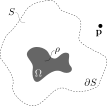
\includegraphics[width=0.4\linewidth]{figs/fuentes-equivalentes.pdf}
    \caption{
        Distribución de masa tridimensional con densidad $\rho$ dentro de una
        región $\Omega$, junto con superficie equipotencial $\partial S$ del
        potencial gravitatorio generado por la misma y un punto de observación
        $\mathbf{p}$ exterior a la región $S$ interior a $\partial S$.
    }
    \label{fig:fuentes-equivalentes}
\end{figure}

Considerando que la densidad $\rho$ es nula fuera de la región $\Omega$,
podemos simplificar el dominio de integración de la integral volumétrica.
De esta manera, ambos términos equivalen al valor que asume el potencial $V$ en
el punto $\mathbf{p}$ (ec.~\ref{eq:potencial-gravitatorio-integral}):
%
\begin{equation}
    V(\mathbf{p}) =
    G \int\limits_\Omega
        \frac{\rho(\mathbf{q})}{\left\lVert \mathbf{p} - \mathbf{q}
            \right\rVert}
    \diff v
    =
    G \oint\limits_{\partial S}
        \frac{\sigma(\mathbf{q})}{\left\lVert \mathbf{p} - \mathbf{q}
            \right\rVert}
    \diff s.
\end{equation}

Esta relación se conoce como \emph{fuentes equivalentes de Green}
(\emph{Green's equivalent layer} en inglés) y de la cual se deduce que el
potencial que genera una distribución de densidad tridimensional es
indistinguible del que genera una masa superficial (o una capa delgada)
distribuida sobre una superficie equipotencial \citep[][p.~62]{blakely1995}.

Esta propiedad de los campos gravitatorios nos permite desarrollar metodologías
de interpolación de campos armónicos basados en el modelado de distribuciones
de masas arbitrarias, sin necesidad de que guarden relación con las geometrías
y densidades de los cuerpos que generan los campos observados.
Además, las fuentes equivalentes de Green dejan en evidencia la no unicidad de
las fuentes de los campos gravitatorios: existe una infinita cantidad de
distribuciones de masas que pueden generar el mismo campo gravitatorio, o una
aproximación suficiente para resultar indistinguible a efectos prácticos.


\chapter{Tesseroides de densidad variable}


\chapter[Fuentes equivalentes potenciadas por gradiente]{
    Fuentes equivalentes potenciadas por gradiente
}
\chaptermark{Fuentes equiv. potenciadas por gradiente}
\label{cha:eql-gradient-boosted}

Este capítulo es una traducción al español del artículo titulado
\emph{Gradient-boosted equivalent sources} escrito por Santiago R. Soler
y Leonardo Uieda, y publicado en \emph{Geophysical Journal
International} en Agosto de 2021 \citep{soler2021}.
Una preimpresión del artículo se encuentra disponible bajo licencia Creative
Commons Atribución 4.0 Internacional en
\href{https://eartharxiv.org/}{EarthArXiv}:
\url{https://doi.org/10.31223/X58G7C}.


% Import files with parameter values generated by notebooks
\newcommand{\AustraliaSmallAreaEastingSize}{$300 \, \text{km}$}
\newcommand{\AustraliaSmallAreaNorthingSize}{$300 \, \text{km}$}
\newcommand{\AustraliaSmallAreaNPoints}{14934}
\newcommand{\AustraliaDepthMin}{$1000 \, \text{m}$}
\newcommand{\AustraliaDepthMax}{$15000 \, \text{m}$}
\newcommand{\AustraliaDampingMin}{0.01}
\newcommand{\AustraliaDampingMax}{10000}
\newcommand{\AustraliaEqlDepth}{$3000 \, \text{m}$}
\newcommand{\AustraliaEqlDamping}{100}
\newcommand{\AustraliaEqlSpacing}{$1800 \, \text{m}$}
\newcommand{\AustraliaEqlWindowSize}{$225 \, \text{km}$}
\newcommand{\AustraliaEqlRmsScore}{$1.33 \, \text{mGal}$}
\newcommand{\AustraliaEqlNSources}{796744}
\newcommand{\AustraliaEqlGridNLongitude}{2442}
\newcommand{\AustraliaEqlGridNLatitude}{2085}
\newcommand{\AustraliaEqlGridHeight}{$2127.58 \, \text{m}$}\newcommand{\BestAirborneSourceBelowDataConstantDepthDamping}{10$^{-2}$}
\newcommand{\BestAirborneSourceBelowDataConstantDepthDepth}{7000}
\newcommand{\BestAirborneSourceBelowDataConstantDepthRms}{0.35}
\newcommand{\BestAirborneSourceBelowDataConstantDepthNPoints}{5673}
\newcommand{\BestAirborneSourceBelowDataRelativeDepthDamping}{10$^{-2}$}
\newcommand{\BestAirborneSourceBelowDataRelativeDepthDepth}{9000}
\newcommand{\BestAirborneSourceBelowDataRelativeDepthRms}{0.35}
\newcommand{\BestAirborneSourceBelowDataRelativeDepthNPoints}{5673}
\newcommand{\BestAirborneSourceBelowDataVariableDepthDamping}{1}
\newcommand{\BestAirborneSourceBelowDataVariableDepthDepthFactor}{1}
\newcommand{\BestAirborneSourceBelowDataVariableDepthDepth}{1450}
\newcommand{\BestAirborneSourceBelowDataVariableDepthKNearest}{15}
\newcommand{\BestAirborneSourceBelowDataVariableDepthRms}{0.36}
\newcommand{\BestAirborneSourceBelowDataVariableDepthNPoints}{5673}
\newcommand{\BestAirborneBlockAveragedSourcesConstantDepthDamping}{10$^{-4}$}
\newcommand{\BestAirborneBlockAveragedSourcesConstantDepthDepth}{9000}
\newcommand{\BestAirborneBlockAveragedSourcesConstantDepthSpacing}{3000}
\newcommand{\BestAirborneBlockAveragedSourcesConstantDepthRms}{0.34}
\newcommand{\BestAirborneBlockAveragedSourcesConstantDepthNPoints}{1100}
\newcommand{\BestAirborneBlockAveragedSourcesRelativeDepthDamping}{10$^{-3}$}
\newcommand{\BestAirborneBlockAveragedSourcesRelativeDepthDepth}{9000}
\newcommand{\BestAirborneBlockAveragedSourcesRelativeDepthSpacing}{2000}
\newcommand{\BestAirborneBlockAveragedSourcesRelativeDepthRms}{0.34}
\newcommand{\BestAirborneBlockAveragedSourcesRelativeDepthNPoints}{1663}
\newcommand{\BestAirborneBlockAveragedSourcesVariableDepthDamping}{10$^{-2}$}
\newcommand{\BestAirborneBlockAveragedSourcesVariableDepthSpacing}{2000}
\newcommand{\BestAirborneBlockAveragedSourcesVariableDepthDepthFactor}{2}
\newcommand{\BestAirborneBlockAveragedSourcesVariableDepthDepth}{50}
\newcommand{\BestAirborneBlockAveragedSourcesVariableDepthKNearest}{15}
\newcommand{\BestAirborneBlockAveragedSourcesVariableDepthRms}{0.33}
\newcommand{\BestAirborneBlockAveragedSourcesVariableDepthNPoints}{1663}
\newcommand{\BestAirborneGridSourcesConstantDepthDamping}{10$^{-1}$}
\newcommand{\BestAirborneGridSourcesConstantDepthDepth}{7000}
\newcommand{\BestAirborneGridSourcesConstantDepthSpacing}{1000}
\newcommand{\BestAirborneGridSourcesConstantDepthRms}{0.34}
\newcommand{\BestAirborneGridSourcesConstantDepthNPoints}{12544}\newcommand{\BestGroundSourceBelowDataConstantDepthDamping}{10$^{-1}$}
\newcommand{\BestGroundSourceBelowDataConstantDepthDepth}{7000}
\newcommand{\BestGroundSourceBelowDataConstantDepthRms}{0.78}
\newcommand{\BestGroundSourceBelowDataConstantDepthNPoints}{963}
\newcommand{\BestGroundSourceBelowDataRelativeDepthDamping}{10$^{-1}$}
\newcommand{\BestGroundSourceBelowDataRelativeDepthDepth}{9000}
\newcommand{\BestGroundSourceBelowDataRelativeDepthRms}{0.79}
\newcommand{\BestGroundSourceBelowDataRelativeDepthNPoints}{963}
\newcommand{\BestGroundSourceBelowDataVariableDepthDamping}{1}
\newcommand{\BestGroundSourceBelowDataVariableDepthDepthFactor}{1}
\newcommand{\BestGroundSourceBelowDataVariableDepthDepth}{1000}
\newcommand{\BestGroundSourceBelowDataVariableDepthKNearest}{15}
\newcommand{\BestGroundSourceBelowDataVariableDepthRms}{0.80}
\newcommand{\BestGroundSourceBelowDataVariableDepthNPoints}{963}
\newcommand{\BestGroundBlockAveragedSourcesConstantDepthDamping}{10$^{-1}$}
\newcommand{\BestGroundBlockAveragedSourcesConstantDepthDepth}{7000}
\newcommand{\BestGroundBlockAveragedSourcesConstantDepthSpacing}{3000}
\newcommand{\BestGroundBlockAveragedSourcesConstantDepthRms}{0.77}
\newcommand{\BestGroundBlockAveragedSourcesConstantDepthNPoints}{518}
\newcommand{\BestGroundBlockAveragedSourcesRelativeDepthDamping}{10$^{-1}$}
\newcommand{\BestGroundBlockAveragedSourcesRelativeDepthDepth}{7000}
\newcommand{\BestGroundBlockAveragedSourcesRelativeDepthSpacing}{3000}
\newcommand{\BestGroundBlockAveragedSourcesRelativeDepthRms}{0.79}
\newcommand{\BestGroundBlockAveragedSourcesRelativeDepthNPoints}{518}
\newcommand{\BestGroundBlockAveragedSourcesVariableDepthDamping}{10$^{-1}$}
\newcommand{\BestGroundBlockAveragedSourcesVariableDepthSpacing}{3000}
\newcommand{\BestGroundBlockAveragedSourcesVariableDepthDepthFactor}{1}
\newcommand{\BestGroundBlockAveragedSourcesVariableDepthDepth}{600}
\newcommand{\BestGroundBlockAveragedSourcesVariableDepthKNearest}{15}
\newcommand{\BestGroundBlockAveragedSourcesVariableDepthRms}{0.72}
\newcommand{\BestGroundBlockAveragedSourcesVariableDepthNPoints}{518}
\newcommand{\BestGroundGridSourcesConstantDepthDamping}{10$^{2}$}
\newcommand{\BestGroundGridSourcesConstantDepthDepth}{3000}
\newcommand{\BestGroundGridSourcesConstantDepthSpacing}{2000}
\newcommand{\BestGroundGridSourcesConstantDepthRms}{0.97}
\newcommand{\BestGroundGridSourcesConstantDepthNPoints}{3192}\newcommand{\BoostOverlappingWindowSize}{$30000 \, \text{m}$}\newcommand{\EqlBoostAirborneRmsScore}{$0.38 \, \text{mGal}$}
\newcommand{\EqlBoostAirborneDepth}{$3000 \, \text{m}$}
\newcommand{\EqlBoostAirborneDamping}{0.1}
\newcommand{\EqlBoostAirborneSpacing}{$2 \, \text{km}$}
\newcommand{\EqlBoostAirborneWindowSize}{$20 \, \text{km}$}
\newcommand{\EqlBoostAirborneNSources}{1663}
\newcommand{\EqlBoostAirborneMinDepth}{$1000 \, \text{m}$}
\newcommand{\EqlBoostAirborneMaxDepth}{$19000 \, \text{m}$}
\newcommand{\EqlBoostAirborneMinDamping}{10$^{-6}$}
\newcommand{\EqlBoostAirborneMaxDamping}{10}\newcommand{\AirborneSourceBelowDataConstantDepthDamping}{10$^{-4}$, 10$^{-3}$,$\dots$, 10$^{2}$}
\newcommand{\AirborneSourceBelowDataConstantDepthDepth}{1000 to 17000, step size 2000}
\newcommand{\AirborneSourceBelowDataRelativeDepthDamping}{10$^{-4}$, 10$^{-3}$,$\dots$, 10$^{2}$}
\newcommand{\AirborneSourceBelowDataRelativeDepthDepth}{1000 to 17000, step size 2000}
\newcommand{\AirborneSourceBelowDataVariableDepthDamping}{10$^{-4}$, 10$^{-3}$,$\dots$, 10$^{2}$}
\newcommand{\AirborneSourceBelowDataVariableDepthDepthFactor}{1 to 6, step size 1}
\newcommand{\AirborneSourceBelowDataVariableDepthDepth}{50 to 1450, step size 200}
\newcommand{\AirborneSourceBelowDataVariableDepthKNearest}{1, 5, 10 and 15}
\newcommand{\AirborneBlockAveragedSourcesConstantDepthDamping}{10$^{-4}$, 10$^{-3}$,$\dots$, 10$^{2}$}
\newcommand{\AirborneBlockAveragedSourcesConstantDepthDepth}{1000 to 17000, step size 2000}
\newcommand{\AirborneBlockAveragedSourcesConstantDepthSpacing}{1000, 2000, 3000 and 4000}
\newcommand{\AirborneBlockAveragedSourcesRelativeDepthDamping}{10$^{-4}$, 10$^{-3}$,$\dots$, 10$^{2}$}
\newcommand{\AirborneBlockAveragedSourcesRelativeDepthDepth}{1000 to 17000, step size 2000}
\newcommand{\AirborneBlockAveragedSourcesRelativeDepthSpacing}{1000, 2000, 3000 and 4000}
\newcommand{\AirborneBlockAveragedSourcesVariableDepthDamping}{10$^{-4}$, 10$^{-3}$,$\dots$, 10$^{2}$}
\newcommand{\AirborneBlockAveragedSourcesVariableDepthSpacing}{1000, 2000, 3000 and 4000}
\newcommand{\AirborneBlockAveragedSourcesVariableDepthDepthFactor}{1 to 6, step size 1}
\newcommand{\AirborneBlockAveragedSourcesVariableDepthDepth}{50 to 1450, step size 200}
\newcommand{\AirborneBlockAveragedSourcesVariableDepthKNearest}{1, 5, 10 and 15}
\newcommand{\AirborneGridSourcesConstantDepthDamping}{10$^{-3}$, 10$^{-2}$,$\dots$, 10$^{2}$}
\newcommand{\AirborneGridSourcesConstantDepthDepth}{1000 to 9000, step size 2000}
\newcommand{\AirborneGridSourcesConstantDepthSpacing}{1000, 2000 and 3000}\newcommand{\GroundSourceBelowDataConstantDepthDamping}{10$^{-4}$, 10$^{-3}$,$\dots$, 10$^{2}$}
\newcommand{\GroundSourceBelowDataConstantDepthDepth}{1000 to 17000, step size 2000}
\newcommand{\GroundSourceBelowDataRelativeDepthDamping}{10$^{-4}$, 10$^{-3}$,$\dots$, 10$^{2}$}
\newcommand{\GroundSourceBelowDataRelativeDepthDepth}{1000 to 17000, step size 2000}
\newcommand{\GroundSourceBelowDataVariableDepthDamping}{10$^{-4}$, 10$^{-3}$,$\dots$, 10$^{2}$}
\newcommand{\GroundSourceBelowDataVariableDepthDepthFactor}{0.1, 0.5, 1, 2, 3, 4, 5 and 6}
\newcommand{\GroundSourceBelowDataVariableDepthDepth}{0 to 1400, step size 200}
\newcommand{\GroundSourceBelowDataVariableDepthKNearest}{1, 5, 10 and 15}
\newcommand{\GroundBlockAveragedSourcesConstantDepthDamping}{10$^{-4}$, 10$^{-3}$,$\dots$, 10$^{2}$}
\newcommand{\GroundBlockAveragedSourcesConstantDepthDepth}{1000 to 17000, step size 2000}
\newcommand{\GroundBlockAveragedSourcesConstantDepthSpacing}{1000, 2000, 3000 and 4000}
\newcommand{\GroundBlockAveragedSourcesRelativeDepthDamping}{10$^{-4}$, 10$^{-3}$,$\dots$, 10$^{2}$}
\newcommand{\GroundBlockAveragedSourcesRelativeDepthDepth}{1000 to 17000, step size 2000}
\newcommand{\GroundBlockAveragedSourcesRelativeDepthSpacing}{1000, 2000, 3000 and 4000}
\newcommand{\GroundBlockAveragedSourcesVariableDepthDamping}{10$^{-4}$, 10$^{-3}$,$\dots$, 10$^{2}$}
\newcommand{\GroundBlockAveragedSourcesVariableDepthSpacing}{1000, 2000, 3000 and 4000}
\newcommand{\GroundBlockAveragedSourcesVariableDepthDepthFactor}{0.1, 0.5, 1, 2, 3, 4, 5 and 6}
\newcommand{\GroundBlockAveragedSourcesVariableDepthDepth}{0 to 1400, step size 200}
\newcommand{\GroundBlockAveragedSourcesVariableDepthKNearest}{1, 5, 10 and 15}
\newcommand{\GroundGridSourcesConstantDepthDamping}{10$^{1}$, 10$^{2}$, 10$^{3}$ and 10$^{4}$}
\newcommand{\GroundGridSourcesConstantDepthDepth}{1000 to 9000, step size 2000}
\newcommand{\GroundGridSourcesConstantDepthSpacing}{1000, 2000, 3000 and 4000}\newcommand{\SourceLayoutsSchematicsObservations}{166}
\newcommand{\SourceLayoutsSchematicsSourceBelowData}{166}
\newcommand{\SourceLayoutsSchematicsGridSources}{378}
\newcommand{\SourceLayoutsSchematicsBlockAveragedSources}{87}\newcommand{\NPrisms}{64}
\newcommand{\ModelEasting}{$111319 \, \text{m}$}
\newcommand{\ModelNorthing}{$111319 \, \text{m}$}
\newcommand{\ModelDepth}{$10000 \, \text{m}$}
\newcommand{\ModelMinDensity}{$-900 \, \text{kg} \, \text{m}^{-3}$}
\newcommand{\ModelMaxDensity}{$500 \, \text{kg} \, \text{m}^{-3}$}
\newcommand{\SurveyEasting}{$111319 \, \text{m}$}
\newcommand{\SurveyNorthing}{$110576 \, \text{m}$}
\newcommand{\SurveyNoise}{$1 \, \text{mGal}$}
\newcommand{\GroundSurveyPoints}{963}
\newcommand{\GroundSurveyMinHeight}{$0 \, \text{m}$}
\newcommand{\GroundSurveyMaxHeight}{$2052.2 \, \text{m}$}
\newcommand{\AirborneSurveyPoints}{5673}
\newcommand{\AirborneSurveyMinHeight}{$359 \, \text{m}$}
\newcommand{\AirborneSurveyMaxHeight}{$1255 \, \text{m}$}
\newcommand{\TargetHeight}{$2000 \, \text{m}$}
\newcommand{\TargetSpacing}{$2 \, \text{km}$}
\newcommand{\TargetEastingSize}{57}
\newcommand{\TargetNorthingSize}{56}



\section{Introducción}

Las mediciones de las anomalías en los campos potenciales, como el disturbio de
gravedad o anomalías magnéticas, son ampliamente utilizadas en la exploración
geofísica debido a su bajo costo de adquisición.
Estos datos pueden ser recolectados utilizando sistemas terrestres, aéreos,
marítimos o satelitales.
Durante las mediciones terrestres, los datos son recabados siguiendo
trayectorias irregulares a lo largo de la superficie del terreno, produciendo
altas variaciones en la altitud de los puntos de observación en zonas
montañosas.
Las metodologías aéreas y satelitales obtienen los datos a lo largo de líneas
de vuelo, produciendo mediciones muy próximas espacialmente a lo largo de
trayectorias casi rectas, pero con espaciados mucho mayores entre líneas
adyacentes.
La altitud de observación también puede variar en estos casos debido al
movimiento vertical de la aeronave.
El procesado de estos datos suele incluir interpolaciones sobre grillas
regulares a altitudes constante, tanto para mejorar la visualización con el
objetivo de realizar interpretaciones, así como para preparar los datos para
posteriores procesados y/o modelado (por ejemplo, reducción al polo, cálculo de
derivadas, continuación ascendente, deconvolución de Euler).

Existen muchos métodos en la literatura para realizar interpolaciones en dos
dimensiones, por ejemplo splines de curvatura continua en tensión
\citep{smith1990}, splines biharmónicas (placa delgada) \citep{sandwell1987},
y kriging \citep{hansen1993}.
Estos métodos de propósito general poseen limitaciones a la hora de interpolar
datos provenientes de campos potenciales:
(i)~no son capaces de tomar en cuenta las altitudes de los puntos de
observación,
(ii)~las funciones interpoladoras no son necesariamente harmónicas, siendo esta
la principal presuposición de muchas técnicas de procesado (por ejemplo,
continuación ascendente y derivadas verticales).

Un método ampliamente utilizado para interpolar datos gravitatorios
y magnéticos es la técnica de fuentes equivalentes (también conocida como capa
equivalente -\emph{equivalent layer} en inglés-, funciones de bases radiales
-\emph{radial basis functions} en inglés-, o interpolaciones con funciones de
Green).
Inicialmente introducida por \citet{dampney1969}, el método consiste en ajustar
un modelo de finitas fuentes elementales a los datos observados, y luego usar
ese modelo para predecir nuevos valores.
Además de las interpolaciones, las fuentes equivalentes han sido utilizadas
para realizar reducciones al polo de datos magnéticos \citep{silva1986,
nakatsuka2006, guspi2009}, continuación ascendente \citep{emilia1973, li2010},
procesado conjunto de datos del gradiente gravimétrico \citet{barnes2011},
modelado del campo magnético litosférico \citep{kother2015}, recuperación del
vector de inducción magnética a partir de anomalías magnéticas de campo total
\citep{li2020}, entre otras.

Vale nombrar también el método de colocación por mínimos cuadrados
(\emph{least-squares collocation method} en inglés), ampliamente utilizado en
geodesia.
\citep[][y referencias allí citadas]{tscherning2015}.
Esta metodología se suele aplicar para combinar e interpolar diferentes
funciones lineales de anomalías derivadas del potencial gravitatorio (anomalías
de gravedad, disturbio de gravedad, deflexiones de la vertical, altitud del
geoide, etc.).
Al igual que las fuentes equivalentes, el método de colocación requiere
resolver un sistema lineal grande, cuyo orden equivale a la cantidad de datos
observados.
De esta manera, la aplicación práctica de ambos métodos sufren de los mismos
desafíos computacionales.

Muchas variantes de la técnica de fuentes equivalentes han sido propuestas,
usualmente intentando obtener soluciones más precisas o en menor tiempo.
Los factores claves que varían entre ellos son: (i) el tipo de fuente, (ii) la
ubicación de las fuentes, y (iii) la estrategia de solución.

Los tipos de fuentes más utilizados son masas puntuales para datos
gravitatorios o dipolos para datos magnéticos \citep[e.g.,~][]{vonfrese1981,
silva1986, mendonca1994, siqueira2017}.
Sin embargo, también se han utilizado exitosamente prismas rectangulares
\citep[por~ej.,][]{barnes2011, jirigalatu2019, li2020} y tesseroides
\citep{bouman2016}.
De hecho, incluso fuentes puntuales en conjunto con funciones simple como la
inversa de la distancia, en vez del campo gravitatorio o magnético, pueden ser
utilizadas como fuentes equivalentes \citep{cordell1992}.

La ubicación de las fuentes suele elegirse de acuerdo a alguno de las
siguientes estrategias.
El método más común es distribuir las fuentes en una grilla regular a una
profundad constante \citep[por~ej.,~][]{leao1989, barnes2011, oliveira2013}.
Alternativamente, podemos ubicar una fuente debajo de cada punto de observación
\citep[por~ej.,~][]{cordell1992, siqueira2017}.
Algunos trabajos recientes de \citet{li2020} ubican las fuentes en dos capas
superpuestas a profundidades diferentes.

Los coeficientes de las fuentes equivalentes suelen ser estimados mediante
mínimos cuadrados ponderados.
Esto implica una carga computacional alta cuando la cantidad de datos es grande
(por ej. muestras aéreas o satelitales).
Para reducir la carga computacional, \citet{mendonca1994} construyen la
solución iterativamente al tratar un solo dato al mismo tiempo utilizando el
concepto de \emph{dato equivalente}.

\citet{leao1989} procesan los datos de entrada mediante una ventana móvil, solo
ajustando los datos dentro de la ventana y prediciendo las observaciones en su
centro.
\citet{li2010} y \citet{barnes2011} aplican diferentes operaciones para generar
una representación dispersa de la matriz de sensibilidades (\emph{wavelet
compression} y \emph{quadtree discretization}, respectivamente), lo cual mejora
significativamente la velocidad de ejecución del algoritmo de mínimos
cuadrados.
\citet{oliveira2013} parametrizan las fuentes equivalentes como una función
polinomial bivariada a trazos, reduciendo el número de parámetros en la
solución.
\citet{siqueira2017} desarrollaron una solución iterativa en la cual la matriz
de sensibilidades es transformada en una matriz diagonal con términos
constantes a través del concepto de \emph{exceso de masa}.
\citet{jirigalatu2019} aplican el método Gauss-FFT para acelerar las
operaciones vinculadas al modelado directo y resuelven el problema de mínimos
cuadrados utilizando el descenso del gradiente con el objetivo de evitar
calcular las matrices Hessianas y resolver sistemas lineales.


Muchos de los métodos existentes resuelven problemas subdeterminados,
requiriendo un número mayor de fuentes equivalentes que de cantidad de datos.
Algunos de ellos alcanzan mayores eficiencias al
restringir su aplicación a tipos de datos específicos \citep{siqueira2017},
realizar las interpolaciones sobre grillas regulares \citep{leao1989},
o requieren datos ya grillados \citep{takahashi2020},
por nombrar algunos.
Además, muchas de las optimizaciones propuestas son complejas de implementar en
un programa de computación, limitando que sean ampliamente utilizados.

En el presente trabajo, proponemos dos estrategias para reducir el costo
computacional de la técnica de fuentes equivalentes:

\begin{enumerate}
    \item Reducir el número de fuentes equivalentes para muestras con
        sobremuestreo mediante una estrategia de \emph{promedio en
        bloques} (\emph{block-averaging} en inglés), manteniendo la calidad de
        la solución.
    \item Ajustar el modelo de fuentes equivalentes iterativamente sobre
        ventanas solapadas utilizando un algoritmo de \emph{potenciación del
        gradiente} (\emph{gradient-boosting} en inglés) \citep{friedman2001}.
\end{enumerate}

La primera estrategia consiste en dividir el área de estudio en bloques
y asignar una única fuente a cada bloque, localizada en la ubicación media de
los puntos de datos.
Para muestras aéreas, navales y satelitales, las cuales presentan sobremuestreo
a lo largo de la trayectoria del vehículo, esto puede reducir considerablemente
el tamaño del problema inverso manteniendo a su vez la misma calidad en la
interpolación.

El algoritmo de \emph{potenciación del gradiente} permite ajustar el modelo de
fuentes equivalentes de manera iterativa, operando de manera individual sobre
cada una de las ventanas con solapamiento.
Como resultado, nuestro método resuelve muchos problemas de mínimos cuadrados
de menor tamaño en vez de un único gran problema.
Este posee algunas semejanzas con la estrategia utilizada por \citet{leao1989},
pero sin el requerimiento de que tanto las fuentes como los puntos de
interpolación se encuentren en grillas regulares.

Mediantes pruebas sobre datos sintéticos, mostramos que:
(i)~las fuentes \emph{promediadas en bloque} son capaces de alcanzar el mismo
nivel de precisión que otras disposiciones de fuentes equivalentes más
tradicionales, utilizando una fracción del número de fuentes; y
(ii)~el algoritmo \emph{potenciación del gradiente} reduce significativamente la
memoria necesaria para ajustar grandes cantidades de datos, sin sacrificar
precisión en las predicciones.
Finalmente, una combinación de ambas estrategias es utilizada para procesar una
colección de aproximadamente 1.7 millones de datos de gravedad tomados sobre la
superficie de Australia.

%%%%%%%%%%%%%%%%%%%%%%%%%%%%%%%%%%%%%%%%%%%%%%%%%%%%%%%%%%%%%%%%%%%%%%%%%%%%%%%

\section{Metodología}

\subsection{La técnica de fuentes equivalentes}
\label{sec:equivalent-sources-technique}

De aquí en más seguiremos las \emph{fuentes equivalentes generalizadas}
propuestas por \citet{cordell1992}
y asumiremos que cualquier función harmónica $d(\mathbf{p})$
puede ser aproximada por la suma de los efectos de $M$ fuentes puntuales

\begin{equation}
    d(\mathbf{p})
    =
    \sum\limits_{j=1}^{M} \frac{c_j}{| \mathbf{p} - \mathbf{q}_j
    |} \ ,
    \label{eq:eql-forward}
\end{equation}

\noindent donde $\mathbf{p}$ y $\mathbf{q}_j$ son, respectivamente, los
vectores posición de datos y fuentes en un espacio cartesiano tridimensional,
y $c_j$ es un coeficiente escalar relacionado con la masa puntual localizada en
$\mathbf{q}_j$.
En la sección~\ref{sec:source_distribution} realizamos una discusión acerca de
la distribución horizontal y vertical de las fuentes.

En caso de que poseamos mediciones de nuestra función harmónica en $N$ puntos
de observación
$\{\mathbf{p}_1\ \mathbf{p}_2\ \ldots\ \mathbf{p}_N\}$,
podemos escribir un sistema de $N$ ecuaciones de la forma:

\begin{equation}
    d_i
    =
    \sum\limits_{j=1}^{M} \frac{c_j}{| \mathbf{p}_i - \mathbf{q}_j
    |}
    \quad \forall i=1,2,\ldots,N
    \ ,
    \label{eq:forward-sum}
\end{equation}

\noindent donde $d_i$ es el efecto de las fuentes sobre el punto
$\mathbf{p}_i$.
Estas ecuaciones pueden ser expresadas de forma matricial como:

\begin{equation}
    \mathbf{d} = \mathbf{A} \mathbf{c} \ ,
    \label{eq:linear-problem}
\end{equation}

\noindent donde $\mathbf{d}$ es un vector columna que contiene los $N$ valores
predichos sobre cada punto de observación,
$\mathbf{c}$ es un vector columna formado por los $M$ coeficientes $c_j$ y
$\mathbf{A}$ es la matriz Jacobiana de $N \times M$ elementos,
los cuales se definen como:

\begin{equation}
    a_{ij} = \frac{1}{|\mathbf{p}_i - \mathbf{q}_j|}
\end{equation}

Para un conjunto de $N$ observaciones $\mathbf{d}^o$, podemos hallar la
solución de la ecuación~\ref{eq:linear-problem} mediante mínimos cuadrados y de
esa manera obtener los valores de
$\mathbf{c}$ que mejor ajustan a las observaciones.
Estos coeficientes pueden ser, a su vez, utilizados para predecir los valores
de la función harmónica en cualquier otro punto externo a las fuentes,
evaluando la ecuación~\ref{eq:eql-forward}.
El grillado o la continuación ascendente puede entonces ser realizados mediante
predicciones sobre puntos de una grilla regular o sobre puntos a diferentes
altitudes, respectivamente.


\subsection{Solución por mínimos cuadrados amortiguados}
\label{sec:eql_inversion}

Es posible obtener los valores de los coeficientes $\mathbf{c}$ que mejor
ajustan a los valores observados $\mathbf{d}^o$ minimizando la función objetivo

\begin{equation}
    \phi(\mathbf{c}) =
    \left[\mathbf{d}^o - \mathbf{A}\mathbf{c}\right]\trans
    \mathbf{W}
    \left[\mathbf{d}^o - \mathbf{A}\mathbf{c}\right]
    + \lambda_d\ \mathbf{c}\trans\mathbf{c}
    \ ,
    \label{eq:misfit-unscaled}
\end{equation}

\noindent donde
$\mathbf{W}$ es una matriz diagonal de $N \times N$ elementos que contiene los
pesos ponderados de los datos observados, y
$\lambda_d$ es el parámetro de \emph{amortiguamiento} (\emph{damping} en
inglés), mayor que cero y con las mismas unidades que los elementos de la
matriz Jacobiana.

El segundo término del miembro derecho de la ecuación~\ref{eq:misfit-unscaled}
consiste en una regularización Thikhonov de orden cero \citep{tikhonov1977},
también conocida como regularización de amortiguamiento (\emph{damping
regularization}), que se utiliza para estabilizar la solución.

El parámetro de amortiguamiento controla cuánta regularización será aplicada.
Un valor muy grande generaría soluciones muy suaves que fallarían en reproducir
las componentes de altas frecuencias presente en los datos, mientras que un
valor muy pequeño resultaría en un sobreajuste, produciendo resultados de
interpolación irreales
\citep{martinez2016}.
El rango de valores aceptables para el parámetro de amortiguamiento
$\lambda_d$ dependerá de los valores de la matriz Jacobiana $\mathbf{A}$
y de los coeficientes.
Por lo tanto, este rango puede variar (considerablemente en muchas ocasiones)
entre diferentes conjuntos de datos, haciendo difícil una apropiada elección en
la práctica.

Para resolver esta problema, primero escalaremos la matriz Jacobiana de forma
tal que sus elementos sean adimensionales y que cada columna posea varianza
unitaria.
Definimos la matriz diagonal $\mathbf{S}$ como:

\begin{equation}
    \mathbf{S} =
    \begin{bmatrix}
      \sigma_1 & 0 & \cdots &0 \\
      0 & \sigma_2 & \cdots &0 \\
      \vdots & \vdots & \ddots & \vdots \\
      0  & 0 & \cdots & \sigma_M
    \end{bmatrix}_{M \times M}
    ,
\end{equation}

\noindent donde $\sigma_j$ es la desviación estándar de la columna $j$-ésima
de la matriz $\mathbf{A}$.
Luego reescribimos el problema directo de la ecuación~\ref{eq:linear-problem}
como:

\begin{equation}
    \mathbf{d}
    =
    \mathbf{A} \mathbf{S}\inv \mathbf{S} \mathbf{c}
    =
    \Big[
        \mathbf{A} \mathbf{S}\inv
    \Big]
    \Big[
        \mathbf{S} \mathbf{c}
    \Big]
    =
    \mathbf{B} \mathbf{m}
\end{equation}

\noindent donde $\mathbf{B} = \mathbf{A} \mathbf{S}\inv$ es la matriz Jacobiana
escalda y adimensional, y
$\mathbf{m} = \mathbf{S} \mathbf{c}$ es el vector que contiene los coeficientes
escalados cuyas unidades son las mismas que la de los datos.

La función objetivo definida en la ecuación~\ref{eq:misfit-unscaled} puede ser
reescrita como:

\begin{equation}
    \phi(\mathbf{m}) =
    \left[\mathbf{d}^o - \mathbf{B}\mathbf{m}\right]\trans
    \mathbf{W}
    \left[\mathbf{d}^o - \mathbf{B}\mathbf{m}\right]
    + \lambda\ \mathbf{m}\trans\mathbf{m}
    \ ,
    \label{eq:misfit}
\end{equation}

\noindent donde $\lambda$ es un parámetro de \emph{amortiguamiento
adimensional} y la regularización es aplicada a los coeficientes escalados
$\mathbf{m}$ en vez de al vector $\mathbf{c}$.
Utilizando un parámetro de amortiguamiento adimensional nos permite limitar el
rango de valores de $\lambda$ que generan las predicciones más precisas,
independientemente del set de datos y sus unidades.
A partir de nuestra experiencia, recomendamos buscar valores de $\lambda$ entre
$10^{-6}$ y $10^{4}$ variando por orden de magnitud.
La elección del amortiguamiento y de otros hiperparámetros, como la profundidad
de las fuentes, puede realizarse a través de métodos estadísticos conocidos,
como la validación cruzada.

El vector de coeficientes escalados $\hat{\mathbf{m}}$ que minimiza la función
objetivo puede hallarse resolviendo el \emph{sistema de ecuaciones normales}
\citep{menke1989}:

\begin{equation}
    \left[
      \mathbf{B}\trans \mathbf{W} \mathbf{B} + \lambda \mathbf{I}
    \right]
    \hat{\mathbf{m}} =
    \mathbf{B}\trans\mathbf{W}
    \mathbf{d}^o.
    \label{eq:least_squares_solution}
\end{equation}

Una vez que los coeficientes escalados son obtenidos, los coeficientes sin
escalar
$\hat{\mathbf{c}}$ pueden ser calculados quitando el factor de escalado:

\begin{equation}
    \hat{\mathbf{c}} = \mathbf{S}\inv \hat{\mathbf{m}} \ .
\end{equation}

\noindent Las operaciones relacionadas al modelado directo que se utilizan para
realizar predicciones (por ejemplo, interpolaciones seguidas de continuaciones
ascendentes) permanecen sin variaciones al utilizar el vector
$\hat{\mathbf{c}}$ en vez de $\hat{\mathbf{m}}$.


\subsection{Potenciación del gradiente}

La potenciación del gradiente fue inicialmente introducida por
\citet{friedman2001, friedman2002} como un método para ajustar modelos
paramétricos de manera aditiva de la siguiente forma:

\begin{equation}
    d = \sum_{k=1}^K \alpha_k f(\mathbf{c}_k),
\end{equation}

\noindent donde $\alpha_k$ es un coeficiente llamado \emph{tamaño de paso}
y $f$ es una función del vector de parámetros $\mathbf{c}_k$.
Para problemas lineales, estos modelos aditivos pueden expresarse según la
siguiente ecuación matricial:

\begin{equation}
    \mathbf{d} = \sum_{k=1}^K \mathbf{A}_k \mathbf{c}_k \ .
    \label{eq:gb-linear-model}
\end{equation}

\noindent Dada la linealidad de la funciones $f(\mathbf{c}_k)$, los parámetros
de tamaño de paso $\alpha_k$ pueden ser incluidos en el vector de parámetros
$\mathbf{c}_k$.

Aplicando esta técnica al problema de fuentes equivalentes, podemos transformar
la ecuación~\ref{eq:linear-problem} en un modelo aditivo siguiendo estos
pasos:

\begin{enumerate}
  \item Definir un conjunto de $M$ fuentes equivalentes distribuidas a lo
      largo de la zona de estudio (ver sección~\ref{sec:source_distribution}
      para más detalles).
  \item Definir un conjunto de $K$ ventanas solapadas de igual tamaño que
      cubren toda la zona de estudio.
  \item Crear $K$ conjuntos distintos de fuentes equivalentes, uno por cada
      ventana.
      Cada conjunto estará conformado por la proción de las $M$ fuentes
      originales que caen dentro de la respectiva ventana.
      Dado que las ventanas se solapan, el número total de fuentes considerando
      cada uno de los conjuntos será mayor que $M$.
  \item Definir el vector $\mathbf{c}_k$ como los $M_k$ coeficientes
      correspondientes a las fuentes equivalentes de la ventana $k$-ésima.
  \item Definir la matriz $\mathbf{A}_k$ como la matriz Jacobiana de $N \times
      M_k$ elementos entre las fuentes de la ventana $k$-ésima y todos los $N$
      puntos de datos de la muestra.
  \item Modelar los datos predichos por las fuentes como una superposición de
      los efectos de los $K$ conjuntos de fuentes equivalentes
      (ec.~\ref{eq:gb-linear-model}).
\end{enumerate}

El algoritmo de potenciación del gradiente funciona ajustando cada componente
del modelo aditivo, una a la vez, a los residuos de la componente anterior.
\citet{friedman2001} demuestra que esto corresponde a una optimización por
descenso del gradiente en el \emph{espacio funcional}.
El Algoritmo~\ref{alg:gradient_boosting} presenta nuestra adaptación del
algoritmo de potenciación del gradiente para hallar las soluciones  de los $K$
vectores de parámetros $\mathbf{c}_k$ de la ec.~\ref{eq:gb-linear-model}
mediante mínimos cuadrados amortiguados.

\begin{algorithm}[!h]
  \DontPrintSemicolon
  \linespread{1.5}\selectfont
  Definir el vector residual $\mathbf{r}_{0} = \mathbf{d}^o$ \;
  \For{ $k = 1$ \KwTo $K$ }{


      Calcular la matriz Jacobiana $\mathbf{A}_k$ de $N \times M_k$ elementos
      \;

      $\mathbf{B}_k = \mathbf{A}_k \mathbf{S}_k\inv$
      \nllabel{alg:scale}
      \;

      $
       \hat{\mathbf{m}}_k = \left[\mathbf{B}_k\trans \mathbf{W}_k \mathbf{B}_k +
       \lambda \mathbf{I} \right]\inv \mathbf{B}_k\trans \mathbf{W}_k
       \mathbf{r}_{k-1}
      $
      \nllabel{alg:fit}
      \;

      $\hat{\mathbf{c}}_k = \mathbf{S}_k\inv \hat{\mathbf{m}}_k$
      \nllabel{alg:unscale}
      \;

      $\mathbf{d}_k = \mathbf{A}_k \hat{\mathbf{c}}_k$
      \nllabel{alg:predicted}
      \;

      $\mathbf{r}_k = \mathbf{r}_{k - 1} - \mathbf{d}_k$
      \nllabel{alg:residual}
      \;
  }
  \BlankLine
  \linespread{1}\selectfont
  \caption{
      Solución mediante potenciación del gradiente de una regresión por mínimos
      cuadrados amortiguados.
  }
  \label{alg:gradient_boosting}
\end{algorithm}

Luego de que todo los vectores de coeficientes $\mathbf{c}_k$ fueron estimados,
podemos predecir el efecto del modelo aditivo de fuentes equivalentes mediante
la suma

\begin{equation}
    d(\mathbf{p}) =
    \sum\limits_{k=1}^K \sum\limits_{j=1}^{M_k}
    \frac{{c_k}_j}{| \mathbf{p} - {\mathbf{q}_k}_j |}
    \ ,
    \label{eq:eql-forward-gb}
\end{equation}

\noindent donde ${c_k}_j$ es el $j$-ésimo elemento del vector $\mathbf{c}_k$
y ${\mathbf{q}_k}_j$ es el vector posición de la $j$-ésima fuente de la
$k$-ésima ventana.

Para mejorar la convergencia del algoritmo, \citet{friedman2002} sugiere
introducir aleatoriedad en el proceso de ajuste.
En nuestra adaptación logramos esto aleatorizando el orden en el cual las $K$
ventanas son utilizadas durante el algoritmo de potenciación de gradiente.
La sección~\ref{sec:gb_interpolation} explora los efectos de la aleatorización
sobre la velocidad de convergencia del algoritmo y sobre la precisión de la
interpolación.

Las matrices $\mathbf{A}_k$ poseen solo $N \times M_k$ elementos (donde $M_k$
es la cantidad de fuentes dentro de la ventana $k$-ésima), las cuales pueden
ser considerablemente más pequeñas que la matriz $\mathbf{A}$ con $N \times M$
elementos.
Por lo tanto, el algoritmo de potenciación del gradiente permite ajustar
modelos de fuentes equivalentes cuyas matrices Jacobianas fueran más grandes
que la memoria computacional disponible.
Además, podemos incrementar o disminuir el tamaño de las ventanas según lo
necesario, dependiendo de la cantidad de fuentes en el modelo y de la memoria
disponible.

Podemos mejorar la eficiencia del algoritmo aún más mediante:

\begin{enumerate}
  \item La utilización de solo los $N_k$ puntos de datos que caen dentro de la
      ventana $k$-ésima a la hora de ajustar los coeficientes de las fuentes
      (pasos \ref{alg:scale} y \ref{alg:fit} del
      algoritmo~\ref{alg:gradient_boosting}).
      De esta manera, podemos reemplazar las matrices Jacobianas $\mathbf{A}_k$
      de $N \times M_k$ elementos por matrices $\tilde{\mathbf{A}}_k$ más
      pequeñas de $N_k \times M_k$ elementos.
      Seguiremos utilizando todos los $N$ puntos de datos cuando calculamos los
      valores predichos y los residuos (pasos \ref{alg:predicted}
      y \ref{alg:residual} del algoritmo~\ref{alg:gradient_boosting}).
  \item La operación de modelado directo que se realiza en el paso
      \ref{alg:predicted} puede ser llevada a cabo mediante una suma
      (ec.~\ref{eq:forward-sum}), en vez de un producto matricial, lo cual
      permite evitar almacenar en memoria la matriz $\mathbf{A}_k$ de $N \times
      M_k$ elementos.
\end{enumerate}

El Algoritmo~\ref{alg:gradient_boosting_window} sintetiza el definitivo
\textit{algoritmo de fuentes equivalentes potenciadas por gradiente},
incorporando estas últimas modificaciones.
La Figura~\ref{fig:gradient-boosting-schematics} muestra un bosquejo de los
pasos del algoritmo aplicado a un conjunto de puntos de observación que simulan
una muestra sobre el terreno y ubicando una fuente debajo de cada punto de
observación.

\begin{algorithm}[!h]
  \DontPrintSemicolon
  \linespread{1.5}\selectfont
  Definir el vector residual $\mathbf{r}_{0} = \mathbf{d}^o$ \;
  \For{ $k = 1$ \KwTo $K$ }{

      Seleccionar los pesos ponderados $\tilde{\mathbf{W}}_k$ y residuos
      $\tilde{\mathbf{r}}_{k - 1}$ correspondientes a los puntos de datos que
      caen dentro de la $k$-ésima ventana
      \;

      Calcular la matriz Jacobiana $\tilde{\mathbf{A}}_k$ considerando puntos
      de datos y fuentes dentro de la $k$-ésima ventana
      \;

      $\mathbf{B}_k = \tilde{\mathbf{A}}_k \mathbf{S}_k\inv$
      \;

      $
       \hat{\mathbf{m}}_k = \left[
       \mathbf{B}_k\trans \tilde{\mathbf{W}}_k \mathbf{B}_k +
       \lambda \mathbf{I} \right]\inv \mathbf{B}_k\trans \tilde{\mathbf{W}}_k
       \tilde{\mathbf{r}}_{k-1}
      $
      \;

      $\hat{\mathbf{c}}_k = \mathbf{S}_k\inv \hat{\mathbf{m}}_k$
      \;

      Calcular $ \mathbf{d}_k $, donde
      $
      {d_k}_i
      =
      \sum\limits_{j=1}^{M_k} \dfrac{{c_k}_j}{| \mathbf{p}_i -
          {\mathbf{q}_k}_j
      |}
      \quad \forall\ i=1\ \text{to}\ N
      $
      \;

      $\mathbf{r}_k = \mathbf{r}_{k - 1} - \mathbf{d}_k$
      \;
  }
  \BlankLine
  \linespread{1}\selectfont
  \caption{Algoritmo de fuentes equivalentes potenciadas por gradiente.}
  \label{alg:gradient_boosting_window}
\end{algorithm}

\begin{figure}[tb]
    \centering
    \includegraphics[width=\linewidth]{figs/eql-gradient-boosted/gradient-boosting-schematics.pdf}
    \caption{
        Bosquejo del algoritmo de fuentes equivalentes potenciadas por el
        gradiente.
        Los puntos de datos están representados por triángulos azules
        (orientados hacia arriba), las fuentes equivalentes por puntos naranja,
        los residuos por triángulos rojos (orientados hacia abajo), y los
        límites de la ventana actual por líneas negras de a trazos.
        El algoritmo comienza seleccionado los datos y las fuentes que caen
        dentro de la primer ventana y continua estimando los coeficientes de
        estas fuentes utilizando los puntos de datos seleccionados.
        Luego, se calcula el efecto de las fuentes ajustadas sobre todos los
        puntos de observación y usamos los datos para calcular los residuos.
        Se utiliza otra ventana para seleccionar otro conjunto de residuos
        y fuentes, se estiman sus coeficientes utilizando los residuos
        seleccionados en vez de los datos originales.
        Nuevamente, el efecto de las fuentes estimadas es calculado sobre todos
        los puntos de observación y se actualizan los residuos.
        Estos pasos son repetidos para cada ventana en orden aleatorio.
    }
    \label{fig:gradient-boosting-schematics}
\end{figure}

Vale la pena notar que los dos conjuntos de fuentes equivalentes
correspondientes a dos ventanas solapadas contiguas poseen una porción de sus
fuentes las mismas ubicaciones, específicamente aquellas que caen en la
intersección de ambas ventanas.
Esto nos permite interpretar que el algoritmo de potenciación de gradiente
ajusta los coeficientes de las fuentes múltiples veces: una vez por cada
ventana que cubre cada una de las fuentes.
Este hecho puede ser explotado con el objetivo de ahorrar memoria.
En vez de almacenar todos los vectores $\mathbf{c}_k$
(ec.~\ref{eq:gb-linear-model}), podemos inicializar un único vector
$\mathbf{c}$ con ceros, donde cada elemento representa el coeficiente de cada
una de las $M$ fuentes originales.
Luego de cada iteración del algoritmo de potenciación por gradiente, añadimos
los coeficientes estimados $\hat{\mathbf{c}}_k$ a sus correspondientes
elementos del vector
$\mathbf{c}$.
Dado que la función de modelado directo es lineal, podemos calcular el campo
resultante mediante la ec.~\ref{eq:eql-forward} en vez de utiliza la
ec.~\ref{eq:eql-forward-gb}.
De esta forma, la cantidad de memoria necesaria para almacenar el conjunto
completo de coeficientes se limita a un único vector de $M$ elementos.

Nuestro algoritmo de potenciado por el gradiente es similar a la \emph{boostrap
inversion} utilizada por \citet{vonfrese1988}, la cual también ajusta
iterativamente porciones del modelo de fuentes equivalentes a datos residuales.
Las diferencias claves entre este y nuestro método son:
(i)~las fuentes en las porciones de solapamiento de las ventanas son ajustadas
más de una vez, permitiendo al algoritmo autocorregirse en caso de soluciones
de baja calidad sobre alguna de las ventanas;
(ii)~utilizamos solo los datos dentro de las ventanas durante el ajuste, lo
cual permite la aplicación del algoritmo a conjuntos de datos más grandes.


\subsection{Ubicación de las fuentes}
\label{sec:source_distribution}

La cantidad ideal de fuentes y sus ubicaciones, tanto horizontales como
verticales, han sido debatidas desde la concepción de la técnica de fuentes
equivalentes de la mano de \citet{dampney1969}.
Las elecciones que se realizan con respecto a estos parámetros juegan un rol
importante en la precisión de las predicciones y de los recursos
computacionales necesarios para estimar los coeficientes de las fuentes.
Una distribución ideal de fuentes debería ser simultáneamente capaz de
reproducir los datos observados en los puntos de muestreo, realizar
predicciones precisas en locaciones no muestreadas y minimizar el costo
computacional necesario.

Un gran número de fuentes homogéneamente distribuidas a lo largo y ancho de la
zona de estudio son capaces de reproducir los datos observados.
Sin embargo, los costos computacionales pueden ser prohibitivos y los problemas
subdeterminados que generan son susceptibles a sobreajustar a los datos,
resultando en interpolaciones y extrapolaciones de baja calidad.
En el otro extremo, la utilización de pocas fuentes reduciría el costo
computacional, pero el modelo podría ser incapaz de reproducir el espectro
completo de los datos observados.

Las características particulares de cada muestra juegan también un rol
importante en la elección de la distribución de las fuentes equivalentes.
En el caso de muestras tomadas sobre la superficie terrestre, las observaciones
suelen localizarse a lo largo de trayectorias irregulares junto con algunos
puntos dispersos.
La cobertura de la región de muestreo es usualmente despareja, dejando grandes
áreas sin ninguna medición.
Por otro lado, las observaciones realizadas mediante vehículos aéreos suelen
estar localizadas a lo largo de líneas de vuelo casi rectas y con poca
separación.
Las mediciones se suelen tomar a intervalos muy cortos, produciendo una gran
densidad de datos a lo largo de las líneas de vuelo.
Esto genera un sesgo en el muestreo, lo cual puede producir artefactos de
\emph{aliasing} en las grillas posteriores.

\subsubsection{Distribuciones horizontales de las fuentes}

\begin{figure}[tb]
    \includegraphics[width=\linewidth]{figs/eql-gradient-boosted/source-layouts-schematics.pdf}
    \caption{
        Bosquejo de las diferentes distribuciones horizontales para los modelos
        de fuentes equivalentes.
        Los puntos azules representan las ubicaciones de las observaciones,
        y los puntos naranja, las ubicaciones de las fuentes equivalentes según
        las distintas estrategias de distribución.
        (a)~Conjunto de \SourceLayoutsSchematicsObservations{} puntos de
        observación que emulan una muestra terrestre.
        (b)~Ubicación de \SourceLayoutsSchematicsSourceBelowData{} fuentes
        obtenidas mediante la distribución \emph{fuentes debajo de datos}.
        (c)~Ubicación de \SourceLayoutsSchematicsGridSources{} fuentes
        obtenidas mediante la distribución \emph{grilla regular}.
        (d)~Ubicación de \SourceLayoutsSchematicsBlockAveragedSources{} fuentes
        obtenidas mediante la distribución \emph{fuentes promediadas por
        bloque}. Las líneas de a trazos grises representan los bloques
        espaciales dentro de los cuales la localización media de los datos es
        calculada.
    }
    \label{fig:source_layouts}
\end{figure}

Las distribuciones más utilizadas para localizar las fuentes equivalentes
horizontalmente son:

\begin{enumerate}
  \item
    \emph{Fuentes debajo de datos}: una única fuente equivalente es ubicada en
    la misma localización horizontal de cada dato
    (fig.~\ref{fig:source_layouts}b), pero a diferente altitud. Por lo tanto,
    la cantidad de fuentes es igual a la cantidad de observaciones ($M=N$).
  \item
    \emph{Grilla regular}: una distribución homogénea de fuentes debajo de la
    zona de estudio (fig.~\ref{fig:source_layouts}c). En la práctica, esto
    suele generar problemas subdeterminados, ya que se requieren mayores
    cantidades de fuentes que de datos ($M>N$).
\end{enumerate}

En el caso de muestras terrestres, la distribución de \emph{grilla regular}
necesita un espaciado entre los nodos lo suficientemente pequeño para poder ser
capaz de ajustar a los datos observados.
Esto genera una cantidad de fuentes innecesariamente grande en regiones donde
no se han realizado observaciones.
En contraste, la distribución \emph{fuentes debajo de datos} es más propensa
a ajustar de manera precisa a los datos observados haciendo uso de una cantidad
menor de fuentes, y por ende reduciendo el costo computacional.
Sin embargo, cuando esta distribución es aplicada a muestras aéreas, la
distribución \emph{fuentes debajo de datos} ubicará una cantidad
indeseablemente grande de fuentes debajo de las líneas de vuelo.
Esto puede conllevar la generación de efectos de \emph{aliasing} sobre los
valores predichos, como un patrón de rayas paralelas a las líneas de vuelo que
suelen observarse en grillas obtenidas de vuelos aeromagnéticos.
La distribución de \emph{grilla regular} puede evitar estos efectos al
distribuir homogéneamente las fuentes y utilizando una capa de fuentes de
densidades continuas (por ejemplo, prismas rectangulares o tesseroides).

Aquí proponemos un nuevo tipo de distribución horizontal de fuentes
equivalentes que puede simultáneamente reducir el costo computacional y mitigar
algunas de las desventajas de las distribuciones existentes.
En la distribución de \emph{fuentes promediadas por bloque}
(\emph{block-averaged sources} en inglés), cada fuente es ubicada en la
posición media de los puntos de datos que caen dentro de un determinado bloque
espacial (fig.~\ref{fig:source_layouts}d).
Esto se realiza de la siguiente forma:

\begin{enumerate}
    \item Dividir la región de estudio en bloques rectangulares de mismo
        tamaño.
    \item \label{item:median-position} Calcular la media de las posiciones
        horizontales de los puntos de observación que caen dentro de cada
        bloque. Los bloques sin ningún punto de observación son omitidos.
    \item Asignar una fuente puntual a cada posición horizontal media calculada
        en el paso \ref{item:median-position}.
\end{enumerate}

La cantidad total de fuentes creadas por esta nueva distribución será menor que
el número total de observaciones si el tamaño de los bloques es elegido
apropiadamente (asegurándose de que los bloques sean lo suficientemente grandes
como para contener más de un único punto de observación).
El problema sobredeterminado que surge de esta distribución posee un costo
computacional inferior y es menos propenso a sobreajustar los datos, ya que la
complejidad del modelo es menor.
Además, el proceso de \emph{promediado por bloques} puede balancear el
espaciado entre fuentes a lo largo de líneas de vuelo y entre líneas contiguas,
ayudando a reducir los efectos de \emph{aliasing} en las grillas que se
generan.
En la sección~\ref{sec:synthetic_distributions}, demostramos mediante pruebas
sobre datos sintéticos que las \emph{fuentes promediadas por bloque} son
capaces de realizar interpolaciones con una precisión comparable a la obtenida
por las otras dos distribuciones, pero utilizando una fracción de fuentes
equivalentes.


\subsubsection{Profundidad de las fuentes}

\begin{figure}[tb]
    \includegraphics[width=\linewidth]{figs/eql-gradient-boosted/depth_types.pdf}
    \caption{
        Ejemplos de diferentes estrategias para asignar profundidades a las
        fuentes equivalentes.
        Asignaremos una única fuente por cada punto de observación,
        localizándolas en la mismas coordenadas horizontales que los puntos de
        datos.
        Las profundidades de las fuentes son
        (a)~una \emph{profundidad constante} a una determinada coordenada
        vertical,
        (b)~una \emph{profundidad relativa} determinada al desplazar
        uniformemente la coordenada vertical de los puntos de datos hacia
        abajo, y
        (c)~una \emph{profundidad variable} determinada por el desplazamiento
        de la coordenada vertical de los puntos de observación por una cantidad
        proporcional a la distancia media entre fuentes vecinas.
        La distancia entre puntos de datos y sus respectivas fuentes (a)
        depende de la altitud de las observaciones, (b) es constante, y (c) es
        proporcional a la distancia horizontal de las fuentes.
        Vale notar cómo las fuentes agrupadas en el centro del perfil (c) se
        encuentran más someras que sus contrapartes en (b).
    }
    \label{fig:depth_types}
\end{figure}

Es ampliamente conocido de la teoría de potencial que la profundidad de una
fuente puntual influencia la longitud de onda del campo observado en la
superficie.
Esto hace que la profundidad de la fuente sea un parámetro clave que afecta el
producto de la interpolación y otras operaciones realizadas mediante fuentes
equivalentes.
En la literatura podemos encontrar múltiples estrategias diferentes para
asignar profundidad de las fuentes.
Aquí destacaremos las siguientes (fig.~\ref{fig:depth_types}):

\begin{enumerate}
  \item
    \emph{Profundidad constante}:
    La opción más simple es ubicar todas las fuentes a la misma profundidad
    (fig.~\ref{fig:depth_types}a).
    Si las mediciones fueron obtenidas a altitudes significativamente diversas,
    algunas mediciones se encontrarán más distantes a las fuentes que otras,
    lo que podría generar problemas a la hora de reproducir las longitudes de
    onda más cortas en los puntos de grandes altitudes.
 \item
    \emph{Profundidad relativa}:
    Las profundidades de las fuentes se determinan al desplazar la coordenada
    vertical de los puntos de datos hacia abajo por una cantidad constante
    (fig.~\ref{fig:depth_types}b).
    Las fuentes no tendrán todas las mismas coordenadas verticales, pero se
    encontrarán todas a la misma distancia vertical con respecto a los puntos
    de observación.
 \item
    \emph{Profundidad variable}:
    Las profundidades de las fuentes son proporcionales a la distancia
    horizontal entre primeros vecinos de datos o fuentes
    (fig.~\ref{fig:depth_types}c).
    Diferentes variaciones de esta estrategia han sido propuestas
    anteriormente, por ejemplo
    \citet{cordell1992}, \citet{guspi2004}, y \citet{guspi2009}.
    La razón fundamental para utilizar esta estrategia surge en caso de que la
    muestra posea puntos muy agrupados (formando \emph{clusters} o cúmulos) en
    algunas áreas, es posible que deseemos ubicar las fuentes debajo de ellas
    a menores profundidades, con el objetivo de preservar las longitudes de
    onda más cortas presentes en esos datos.
\end{enumerate}

Nuestro enfoque sobre la estrategia de \emph{profundidad variable} será:

\begin{equation}
  z = z_{obs} + \Delta z + \alpha h,
  \label{eq:variable_depth}
\end{equation}

\noindent
donde $z$ es la coordenada vertical (positiva hacia abajo) de una fuente
equivalente,
$\Delta z$ es un desplazamiento relativo en profundidad que se aplica de manera
uniforme a todas las fuentes,
$\alpha$ es un \emph{factor de profundidad} adimensional,
$h$ es la distancia horizontal media a las primeras $k$ fuentes vecinas,
y
$z_{obs}$ es una coordenada vertical relacionada a los puntos de observación
que dependerá de la estrategia horizontal utilizada.
Para \emph{fuentes debajo de datos}, será la coordenada vertical del
punto de observación correspondiente a la fuente.
Para una \emph{grilla regular}, puede ser interpolada a partir de la coordenada
vertical de todos los puntos de datos.
Finalmente, para \emph{fuentes promediadas por bloque} será la coordenada
vertical media de todos los puntos de datos que caen dentro del bloque
correspondiente a la fuente.

En la sección~\ref{sec:synthetic_distributions}, probamos la efectividad de
estas estrategias sobre datos sintéticos.

%%%%%%%%%%%%%%%%%%%%%%%%%%%%%%%%%%%%%%%%%%%%%%%%%%%%%%%%%%%%%%%%%%%%%%%%%%%%%%%

\section{Pruebas sobre datos sintéticos}

\begin{figure}[tb]
    \includegraphics[width=\linewidth]{figs/eql-gradient-boosted/synthetic-survey-layouts.pdf}
    \caption{
        Altitudes de los puntos de observación y valores de gravedad para las
        muestras sintéticas sobre terreno (a-b) y aéreas (c-d).
        Las altitudes están dadas en metros sobre el plano de altitud cero.
        Los datos sintéticos de gravedad están contaminados con ruido Gaussiano
        pseudo-aleatorio con media cero y desviación estándar de
        \SurveyNoise{}.
    }
    \label{fig:synthetic-layouts}
\end{figure}

\begin{figure}[tb]
    \centering
    \includegraphics[width=0.7\linewidth]{figs/eql-gradient-boosted/target-grid.pdf}
    \caption{
        Gráfico de la \emph{grilla objetivo} de datos sintéticos de gravedad.
        La grilla está compuesta por
        \TargetEastingSize{}$\times$\TargetNorthingSize{} puntos
        con un espaciado de \TargetSpacing{}.
        Todos los puntos de la grilla se encuentran a una altitud de
        \TargetHeight{} sobre el plano de altitud cero.
    }
    \label{fig:synthetic-target}
\end{figure}

Hemos utilizado un conjunto de datos sintéticos de gravedad para probar la
precisión de la interpolación entre las diferentes estrategias de distribución
horizontal y vertical de fuentes equivalentes, así como también el desempeño
del algoritmo de fuentes equivalentes potenciadas por gradiente.
Para generar los datos sintéticos hemos creado un modelo de
\NPrisms{} prismas rectangulares, distribuidos a lo largo y ancho de un área de
\ModelEasting{}$\times$\ModelNorthing{} con profundidades variables entre
\ModelDepth{} y cero.
El contraste de densidad de los prismas van desde \ModelMinDensity{} a
\ModelMaxDensity{}.
El modelo incluye prismas de diferentes formas, tamaños y profundidades para
crear disturbio de gravedad con una variedad de longitudes de onda.

Hemos creado dos conjuntos de datos sintéticos a partir del mismo modelo, uno
que simula un muestreo sobre el terreno y otro una campaña aérea
(fig.~\ref{fig:synthetic-layouts}).
Para crear la muestra sintética sobre el terreno hemos elegido una porción de
las observaciones presentes en un conjunto de datos de dominio público sobre
Sudáfrica, disponibles a través del NOAA National Centers for Environmental
Information (NCEI). Para la muestra aérea, utilizamos una porción de la Great
Britain Aeromagnetic Survey adquirida por Hunting Geology and Geophysics Ltd
y Canadian Aeroservices Ltd, entre 1955 y 1965, y puesta a disposición pública
por el British Geological Survey (BGS).
En ambos casos, re-escalamos las coordenadas horizontales de cada porción de
muestra para cubrir un área de \SurveyEasting{}$\times$\SurveyNorthing{},
coincidentes con las dimensiones del modelo sintético.
La muestra sintética sobre el terreno contiene \GroundSurveyPoints{}
observaciones distribuidas en altitudes que van desde \GroundSurveyMinHeight{}
y \GroundSurveyMaxHeight{} (fig.~\ref{fig:synthetic-layouts}a).
La muestra aérea posee \AirborneSurveyPoints{} observaciones a altitudes entre
\AirborneSurveyMinHeight{} y \AirborneSurveyMaxHeight{}
(fig.~\ref{fig:synthetic-layouts}c).

Calculamos la componente vertical de la aceleración gravitatoria generada por
el modelo sintético utilizando el método de \citet{nagy2000, nagy2002} con
recientes modificaciones hechas por \citet{fukushima2020}, como se ha
implementado en el software de código abierto Harmonica \citep{harmonica2021}.
Hemos generado una \emph{grilla objetivo} de
\TargetEastingSize{}$\times$\TargetNorthingSize{} puntos con un espaciado de
\TargetSpacing{} y localizados a una altitud de \TargetHeight{} sobre el plano
de altitud cero (fig.~\ref{fig:synthetic-target}) que nos servirá de referencia
para estimar los errores de las interpolaciones.
Luego generamos los datos sintéticos de aceleración de la gravedad sobre la
muestra sobre el terreno (fig.~\ref{fig:synthetic-layouts}b) y sobre la muestra
aérea (fig.~\ref{fig:synthetic-layouts}d).
Además hemos contaminado estos datos sintéticos con ruido Gaussiano
pseudo-aleatorio con media cero y con desviación estándar de \SurveyNoise{}.


\subsection{Estrategias de distribución de fuentes}
\label{sec:synthetic_distributions}

\begin{figure}[p]
    \includegraphics[width=\linewidth]{figs/eql-gradient-boosted/ground_survey_differences.pdf}
    \caption{
        Gráficos con las diferencias entre la \emph{grilla objetivo} y los
        valores interpolados para la muestra sobre el terreno, producidas por
        cada una de las estrategias de distribución de fuentes.
        Los puntos negros representan la ubicación horizontal de los puntos
        correspondientes a los datos sintéticos.
        La \acs{RMSE} y el número total de fuentes equivalentes para cada
        distribución se encuentran reportadas por encima del respectivo
        gráfico.
    }
    \label{fig:ground-survey-differences}
\end{figure}

\begin{figure}[p]
    \includegraphics[width=\linewidth]{figs/eql-gradient-boosted/airborne_survey_differences.pdf}
    \caption{
        Gráficos con las diferencias entre la \emph{grilla objetivo} y los
        valores interpolados para la muestra aérea, producidas por
        cada una de las estrategias de distribución de fuentes.
        Los puntos negros representan la ubicación horizontal de los puntos
        correspondientes a los datos sintéticos.
        La \acs{RMSE} y el número total de fuentes equivalentes para cada
        distribución se encuentran reportadas por encima del respectivo
        gráfico.
    }
    \label{fig:airborne-survey-differences}
\end{figure}

Hemos investigado el efecto sobre la precisión de las interpolaciones de
diferentes estrategias para distribuir las fuentes equivalentes, tanto
horizontal como verticalmente.
Para hacer esto, hemos utilizado las soluciones por mínimos cuadrados
amortiguados descriptas en la sección~\ref{sec:eql_inversion} (sin potenciación
del gradiente) para interpolar los datos sintéticos
(fig.~\ref{fig:synthetic-layouts}) y comparamos los resultados con los valores
de la \emph{grilla objetivo} (fig.~\ref{fig:synthetic-target}).
Este proceso es repetido para cada una de las combinaciones de distribución
horizontal (\emph{fuentes debajo de datos} y \emph{fuentes promediadas por
bloque}) y tipo de profundidad (\emph{constante}, \emph{relativa},
y \emph{variable}), y para fuentes distribuidas en una \emph{grilla regular}
con profundidad constante.
En total se generan 7 diferentes tipos de combinaciones.

Cada estrategia de distribución de fuentes requiere seleccionar valores para
determinados hiperparámetros necesarios para construir, en cada caso, el
conjunto de fuentes equivalentes.
Por ejemplo, al utilizar una profundidad constante necesitamos definir la
profundidad de las fuentes, y si la combinamos con \emph{fuentes promediadas
por bloques} se requiere el tamaño de los bloques.
Las capacidades predictivas de las fuentes equivalentes depende de la elección
de estos hiperparámetros.
Para garantizar que nuestras comparaciones sean justas, llevamos a cabo
exhaustivas búsquedas sobre las combinaciones de los hiperparámetros
(incluyendo el parámetro de \emph{amortiguamiento} de la ec.~\ref{eq:misfit})
con el objetivo de obtener las mejores predicciones que puedan ser alcanzadas
por cada estrategia de distribución de fuentes.
La mejor predicción se define como aquella que minimiza la \ac{RMSE} entre los
valores interpolados y los valores de la \emph{grilla objetivo}
(fig.~\ref{fig:synthetic-target}).
Los valores para cada uno de los parámetros utilizados en estas búsquedas
y aquellos que producen la menor \ac{RMSE} se exponen en las
Tablas~\ref{tab:parameters-ground-survey}
y~\ref{tab:parameters-airborne-survey}.

Las Figuras.~\ref{fig:ground-survey-differences}
y~\ref{fig:airborne-survey-differences}
muestran las diferencias entre la \emph{grilla objetivo} y las mejores
predicciones alcanzadas por cada estrategia de distribución de fuentes, tanto
para la muestra sobre el terreno como para la muestra aérea, respectivamente.
En el caso de la muestra sintética sobre el terreno, las distribuciones
horizontales produjeron valores similares de \ac{RMSE} de aproximadamente
0.8\mGal{}, independientemente del tipo de profundidad que se utilice;
a excepción de las fuentes distribuidas sobre una \emph{grilla regular}, la
cual produjo una \ac{RMSE} mayor de
\BestGroundGridSourcesConstantDepthRms{}\mGal{}.
Las diferencias entre la \emph{grilla objetivo} y los valores interpolados son
mayores en regiones con una pobre cobertura de datos.
Los efectos de borde están presentes en todas las estrategias, pero son
notablemente menores para la combinación de \emph{fuentes promediadas por
bloque} con profundidad variable.
En el caso de la muestra aérea, todas las estrategias (incluyendo la grilla
regular) produce valores similares de \ac{RMSE} de aproximadamente 0.3\mGal{}.
Los gráficos de las diferencias entre la \emph{grilla objetivo} y los valores
interpolados son visualmente indistinguibles entre ellos.

%%%%%%%%%%%%%%%%%%%%%%%%%%%%%%%%%%%%%%%%%%%%%%%%%%%%%%%%%%%%%%%%%%%%%%%%%%%%%%%


\subsection{Tamaño de las ventanas y cantidad de solapamiento en potenciación
del gradiente}
\label{sec:window_size_and_overlap}

Hemos analizado la relación entre la precisión de las interpolaciones y el
tiempo de cómputo del algoritmo de fuentes equivalentes potenciadas por el
gradiente en función de dos factores claves: el tamaño de las ventanas y la
cantidad de solapamiento entre ventanas contiguas.
Las comparaciones fueron realizadas contra la solución obtenida por mínimos
cuadrados amortiguados (ec.~\ref{eq:least_squares_solution}, sin potenciación
del gradiente) utilizando los datos provistos por la muestra aérea sintética
(fig.~\ref{fig:synthetic-layouts}c-d).
Para evitar que existan sesgos en los resultados, utilizamos las mismas
ubicaciones para las fuentes equivalentes tanto como para las interpolaciones
con y sin potenciación del gradiente.
Más precisamente, elegimos fuentes promediadas por bloques con un tamaño de
bloque de
\BestAirborneBlockAveragedSourcesRelativeDepthSpacing\m{} y una profundidad
relativa de
\BestAirborneBlockAveragedSourcesRelativeDepthDepth\m{}.

\subsubsection{Tamaño de las ventanas}
\label{sec:window_size}

El tamaño de las ventanas controla el tamaño de las matrices Jacobianas
$\tilde{\mathbf{A}}_k$ al limitar la cantidad de puntos de datos y fuentes
equivalentes que se utilizan en cada paso del algoritmo de potenciación del
gradiente
(alg.~\ref{alg:gradient_boosting_window}).
Por lo tanto, ventanas pequeñas reducen la cantidad total de memoria necesaria
para estimar los coeficientes de las fuentes.
Sin embargo, estas pueden producir interpolaciones menos precisas al no ser
capaces de alcanzar el mínimo global de la función objetivo en la
ec.~\ref{eq:misfit}.
El tamaño de la ventana también impacta en el tiempo de cómputo de formas poco
intuitivas, ya que ventanas pequeñas generan problemas de mínimos cuadrados más
simples, pero también requieren mayor cantidad de iteraciones del algoritmo de
potenciación del gradiente.

Hemos calculado la \ac{RMSE} de las interpolaciones (entre el resultado de la
interpolación y la \emph{grilla objetivo} de la
fig.~\ref{fig:synthetic-target}) y registramos los tiempos de cómputo
utilizando un valor fijo de solapamiento entre ventanas de 50\% y varios
tamaños de ventanas diferentes.
Para evitar sesgos introducidos por un determinado ordenamiento aleatorio
particular de las ventanas, los cálculos fueron repetidos utilizando diferentes
\emph{semillas} para el generado de números pseudo-aleatorios.
La Figura~\ref{fig:gradient-boosted-comparison}a
muestra la \ac{RMSE}, y
la Figura~\ref{fig:gradient-boosted-comparison}c
el tiempo de cómputo requerido para estimar los coeficientes de las fuentes,
ambos en función del tamaño de las ventanas.

\begin{figure}[tb]
    \includegraphics[width=\linewidth]{figs/eql-gradient-boosted/gradient-boosted-comparisons.pdf}
    \caption{
        \acs{RMSE} de las interpolaciones (a-b) y los tiempos de cómputos
        relativos (c-d) para fuentes equivalentes regulares (líneas naranja de
        a trazos) y para fuentes equivalentes potenciadas por gradiente
        (puntos azules con barras de error).
        El solapamiento de las ventanas se muestra como un porcentaje del
        tamaño de la ventana (un solapamiento del 50\% significa que dos
        ventanas contiguas comparten un área igual a la mitad del tamaño de la
        ventana completa).
        Para las fuentes equivalentes potenciadas por gradiente, la
        \acs{RMSE} y los tiempos de cómputo son valores medios (las barras de
        error corresponden a una desviación estándar) de los resultados
        obtenidos utilizando diferentes semillas para el generador de números
        pseudo-aleatorios.
        Los tiempos de cómputo se muestran como la relación entre el tiempo
        necesario para estimar los coeficientes de las fuentes equivalentes
        potenciadas por el gradiente y el necesario para estimar los
        coeficientes de las fuentes equivalentes regulares.
    }
    \label{fig:gradient-boosted-comparison}
\end{figure}

Estos resultados muestran que los errores de interpolación obtenidos con
potenciación del gradiente son generalmente mayores que el error obtenido por
las fuentes equivalentes regulares.
Los errores decrecen asintóticamente hasta el $\sim 40\%$ de las fuentes
equivalentes regulares para ventanas con un área mayor que el $\sim 10\%$
de la región de estudio.
Los tiempos de cómputo decrecen similarmente con el tamaño de la ventana,
siendo las fuentes potenciadas por gradiente usualmente más rápidas que las
fuentes regulares para ventanas con áreas mayores que el $\sim 5\%$ de la
región de estudio.
A medida que el tamaño de la ventana aumenta, tanto la \ac{RMSE} y el tiempo de
cómputo parece estabilizarse cerca de niveles constantes.

\subsubsection{Solapamiento de las ventanas}

La cantidad de solapamiento entre ventanas contiguas juega un rol importante en
el desempeño de las fuentes potenciadas por gradiente.
Controla la cantidad de iteraciones y cuántas veces una fuente particular será
utilizada en el proceso de ajuste por mínimos cuadrados.
Los experimentos realizados en la sección anterior muestran que un solapamiento
de 50\% es suficiente para alcanzar una precisión aceptable en las
interpolaciones.
Sin embargo, hemos estudiado de forma independiente cómo la cantidad de
solapamiento impacta tanto en la precisión como en el tiempo de cómputo.

Llevamos a cabo un experimento similar al realizado en la
sección~\ref{sec:window_size}, pero esta vez mantuvimos el tamaño de la ventana
fijo a \BoostOverlappingWindowSize{} y variamos la cantidad de solapamiento
entre 0\% y 95\% con un paso de 5\%.
Todos los otros procedimientos experimentales se mantuvieron intactos.
La Figura~\ref{fig:gradient-boosted-comparison}b
muestra la \ac{RMSE} y la
Figura~\ref{fig:gradient-boosted-comparison}d
el tiempo de cómputo requerido para estimar los coeficientes de las fuentes,
ambos en función de la cantidad de solapamiento entre las ventanas.

Nuestros resultados muestran que la \ac{RMSE} de la interpolación decrece con
la cantidad de solapamiento, alcanzando la misma precisión que las fuentes
equivalentes regulares a aproximadamente un solapamiento del 90\%.
Por otro lado, el tiempo de cómputo aumenta con la cantidad de solapamiento,
haciéndose mayor que el necesario por fuentes equivalentes regulares para
solapamientos mayores al 70\%.
Este comportamiento era de esperarse, ya que un aumento en el solapamiento
aumenta la cantidad de iteraciones en el proceso de potenciación del gradiente,
sin reducir el tamaño de los problemas de mínimos cuadrados de forma tal que se
compensen.


\subsection{
    Interpolación con potenciación del gradiente
}
\label{sec:gb_interpolation}

Finalmente, hemos aplicado las fuentes equivalentes potenciadas por gradiente
para interpolar la muestra sintética aérea (fig.~\ref{fig:synthetic-layouts}).
Tal y como hemos realizado anteriormente, utilizamos las fuentes promediadas
por bloque con un tamaño de bloque de \EqlBoostAirborneSpacing{}.
Basado en los resultados de la sección \ref{sec:window_size_and_overlap},
adoptamos un solapamiento entre ventanas contiguas de 50\% y un tamaño de
ventanas de \EqlBoostAirborneWindowSize{}.

Hemos estimado la profundidad relativa de las fuentes y el parámetro de
\emph{amortiguamiento} comparando las predicciones con los valores de la
\emph{grilla objetivo}.
Durante la búsqueda, exploramos valores de profundidad relativa entre
\EqlBoostAirborneMinDepth{} y
\EqlBoostAirborneMaxDepth{} y de valores de \emph{amortiguamiento} entre
\EqlBoostAirborneMinDamping{} y \EqlBoostAirborneMaxDamping{}
de a pasos de un orden magnitud.
Las predicciones más precisas alcanzaron una \ac{RMSE} de
\EqlBoostAirborneRmsScore{} con una profundidad relativa de
\EqlBoostAirborneDepth{} y
un \emph{amortiguamiento} de \EqlBoostAirborneDamping{}.
Vale la pena notar que la \ac{RMSE} alcanzada por las fuentes potenciadas por
gradiente es comparable con los valores obtenidos por las fuentes equivalentes
regulares en la sección~\ref{sec:synthetic_distributions}.
Para resaltar la importancia de aleatorizar el orden en el que se recorren las
ventanas durante la potenciación del gradiente, llevamos a cabo la misma
interpolación una vez más haciendo uso de los mismos valores para la profundidad
relativa y el \emph{amortiguamiento}, pero esta vez iteramos sobre las ventanas
en orden secuencial (de Sur a Norte, de Oeste a Este).

\begin{figure}[t!]
    \centering
    \includegraphics[width=0.7\linewidth]{figs/eql-gradient-boosted/eql-boost-airborne.pdf}
    \caption{
        Error de la interpolación obtenida a partir de fuentes equivalentes
        potenciadas por gradiente utilizando un (a) orden aleatorio y un (b)
        orden secuencial para recorrer las ventanas.
        (a and b)~Mapas de las diferencias entre la \emph{grilla objetivo}
        y los resultados de la interpolación de la muestra sintética aérea.
        La escala de colores fue truncada al mismo rango de valores que la de
        la Figura~\ref{fig:airborne-survey-differences}.
        (c)~\acl{RMSE} luego de cada iteración del algoritmo de potenciación del
        gradiente.
}
\label{fig:eql-boost-airborne}
\end{figure}

Las Figuras~\ref{fig:eql-boost-airborne}a-b
muestran las diferencias entre la \emph{grilla objetivo} y los resultados de la
interpolación obtenida con ventanas en orden aleatorio y en orden secuencial,
respectivamente.
Las diferencias para las ventanas en orden aleatorio se asemejan a las
obtenidas por las fuentes equivalentes regulares que vimos en las
Figuras~\ref{fig:ground-survey-differences}
y \ref{fig:airborne-survey-differences}.
Por otro lado, las diferencias para las ventanas en orden secuencial muestran
una clara tendencia de grandes diferencias negativas hacia el Sur, decreciendo
hacia el Norte.
Esta tendencia se correlaciona con el orden en el que las ventanas son
ejecutadas, con diferencias que van decreciendo en valor absoluto hacia el
final del algoritmo.
La Figura~\ref{fig:eql-boost-airborne}c
muestra la \ac{RMSE} del proceso de ajuste luego de cada iteración, tanto para
ventanas ejecutadas en orden aleatorio como secuencial, indicando claramente
que las ventanas aleatorias generan una convergencia más rápida del algoritmo.


%%%%%%%%%%%%%%%%%%%%%%%%%%%%%%%%%%%%%%%%%%%%%%%%%%%%%%%%%%%%%%%%%%%%%%%%%%%%%%%

\section{Grillado de datos gravimétricos de Australia}

\begin{figure}[p]
    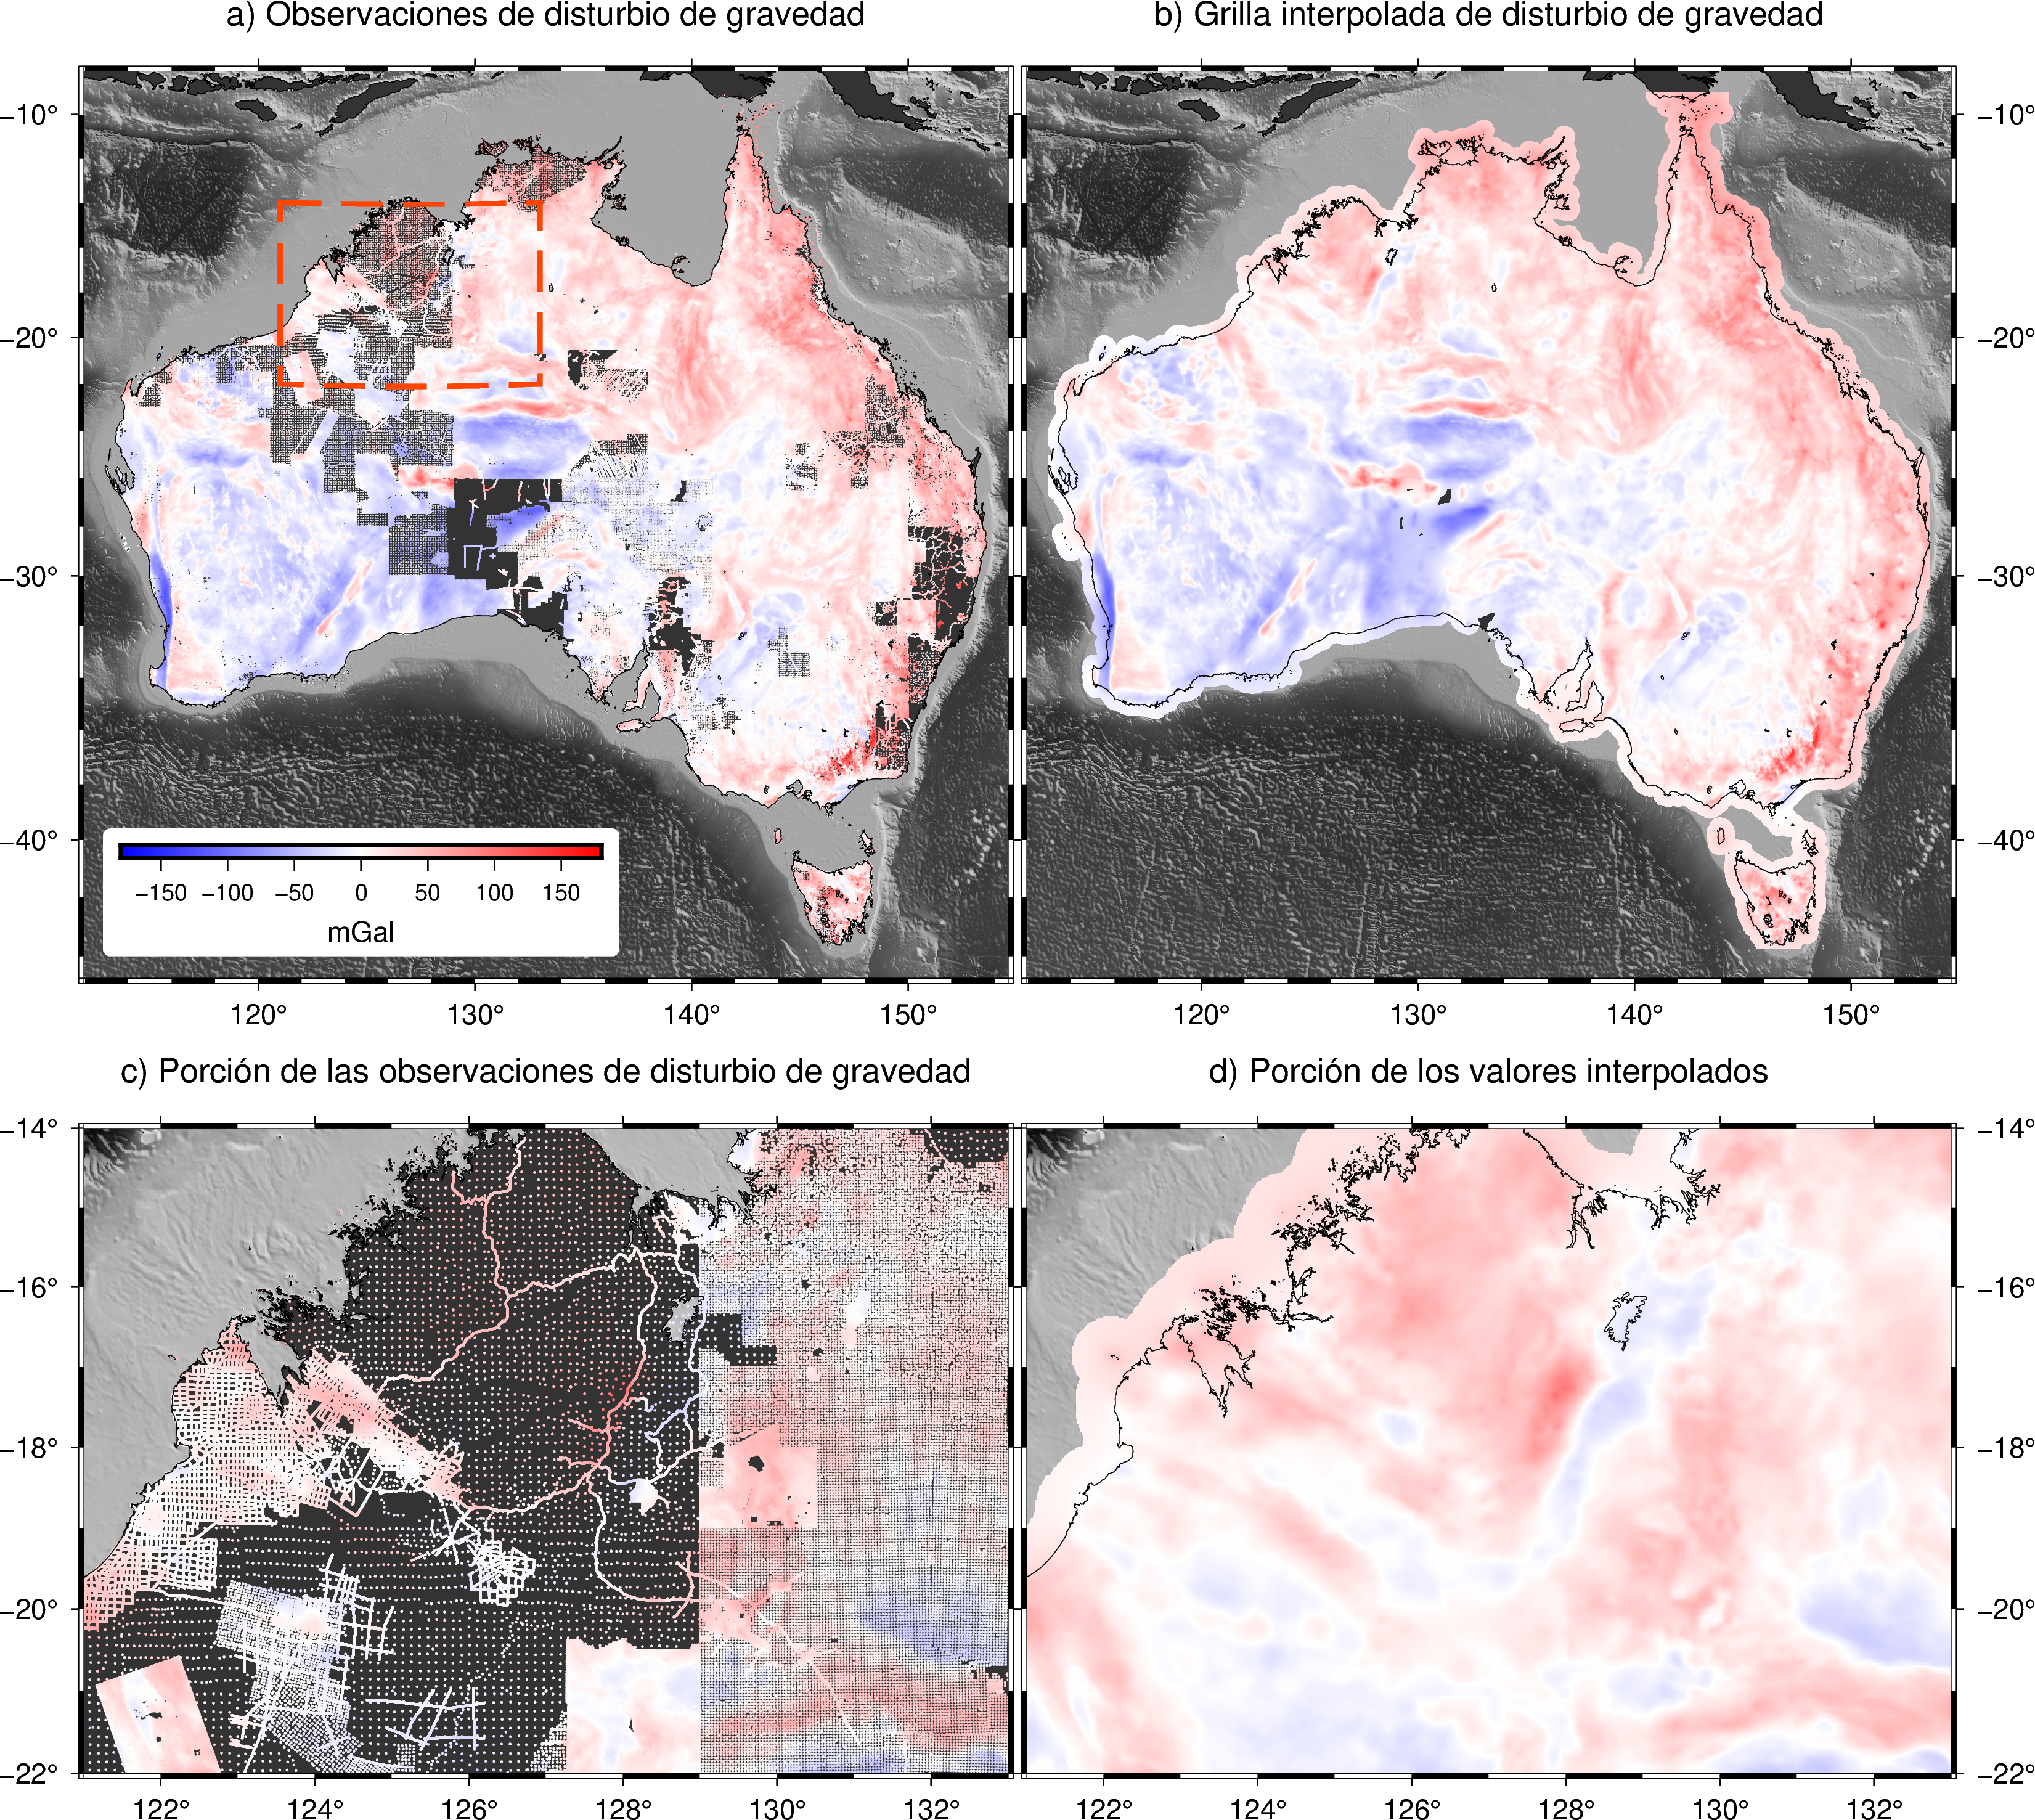
\includegraphics[width=\linewidth]{figs/eql-gradient-boosted/australia.png}
    \caption{
        Mapas de los valores observados (a y c) y valores interpolados (b y d)
        de disturbio de gravedad sobre Australia.
        Los valores observados en a y c se muestran como círculos coloreados.
        El rectángulo rojo con línea de a trazos señala la zona representada en
        los mapas c y d.
        Las observaciones son una porción de una compilación de
        \citet{wynne2018} compuesta por 1.7 millones de mediciones de
        aceleración de la gravedad sobre el terreno.
        Los valores interpolados fueron obtenidos mediante la aplicación de
        fuentes equivalentes potenciadas por gradiente y calculados sobre una
        grilla regular a una altitud de \AustraliaEqlGridHeight{} sobre la
        superficie del elipsoide WGS84.
    }
    \label{fig:australia}
\end{figure}

En esta sección demostraremos cómo podemos utilizar las fuentes equivalentes
potenciadas por gradiente para interpolar grandes cantidades de datos sobre
una grilla regular a una altitud uniforme.
Para esto, hemos seleccionado una compilación de acceso abierto de muestras de
datos de aceleración de gravedad sobre Australia realizada por
\citet{wynne2018} y filtradas y referenciadas al elipsoide WGS84 por
\citet{australia_compilation}.
Contiene 1.7 millones de datos y cubre la mayor parte del territorio
australiano.
Nuestro objetivo es crear una grilla regular de disturbios de gravedad a una
altitud geométrica constante de \AustraliaEqlGridHeight{} (la altitud de
observación más alta presente en los datos).

Hemos calculado el disturbio de gravedad quitando la gravedad normal generada
por el elipsoide WGS84 sobre los datos de gravedad observados
(fig.~\ref{fig:australia}).
Los valores de gravedad normal fueron calculados en cada punto de observación
mediante la fórmula cerrada de \citet{ligotze2001} (ver
sección~\ref{sec:normal-gravity-closed-form}) implementada en la librería Boule
\citep{boule2020}.
Finalmente, transformamos las coordenadas de los puntos de observación a un
sistema de coordenadas planas aplicando una proyección de Mercator.

Comenzamos el proceso de interpolación definiendo un conjunto de \emph{fuentes
promediadas por bloque} haciendo uso de bloques de 1.8\km{} de lado, obteniendo
un total de \AustraliaEqlNSources{}~fuentes puntuales.
El tamaño de los bloques fue elegido para que concuerde con la resolución
deseada para la grilla final (1~minuto de arco equivale aproximadamente
a 1.8\km{} en el ecuador).
Basado en los resultados obtenidos en la
sección~\ref{sec:synthetic_distributions}, elegimos localizar las fuentes
siguiendo la estrategia de \emph{profundidad relativa}.
El solapamiento de las ventanas fue fijado nuevamente a 50\%.
Para determinar el tamaño de las ventanas, calculamos la cantidad de memoria
necesaria para almacenar la matriz Jacobiana más grande que genera el algoritmo
para diferentes valores de tamaño de ventana
(fig.~\ref{fig:australia-memory-cv-error}a).
Hemos seleccionado un tamaño de ventana de \AustraliaEqlWindowSize{} con el
objetivo de limitar la cantidad de memoria por debajo de los 16~Gigabytes.

\begin{figure}[p]
    \centering
    \includegraphics[width=0.6\linewidth]{figs/eql-gradient-boosted/australia-memory-cv-error.pdf}
    \caption{
        (a) Cantidad de memoria computacional necesaria para almacenar la mayor
        matriz Jacobiana en función del tamaño de las ventanas. Nuestra
        implementación de algoritmo almacena los elementos de la matriz como
        puntos flotantes de doble precisión (64 bits).
        (b) \acs{RMSE} entre los valores observados y los valores predichos
        sobre cada punto de observación luego de cada iteración del algoritmo
        de potenciación del gradiente.
        (c) \acs{RMSE} obtenidas de la validación cruzada de K iteraciones para
        pares de valores de \emph{amortiguamiento} y profundidad relativa de
        las fuentes.
        La estrella naranja señala la \acs{RMSE} mínima.
    }
    \label{fig:australia-memory-cv-error}
\end{figure}

Hemos determinados la profundidad relativa de las fuentes y el parámetro de
\emph{amortiguamiento} aplicando una validación cruzada de K iteraciones
(\emph{K-Fold cross-validation} en inglés) mediante la librería scikit-learn
\citep{sklearn2011}.
Este método divide aleatoriamente los datos originales en $k$ conjuntos
(denominados \emph{folds}), ajusta el modelo de fuentes equivalentes utilizando
sólo los datos de $k - 1$ conjuntos y valida el modelo comparando sus
predicciones sobre los puntos pertenecientes al conjunto restante.
Este proceso se lleva a cabo una vez por cada uno de los $k$ conjuntos,
obteniendo una media de las \ac{RMSE} para dicho modelo.
Con el objetivo de acelerar el cómputo, realizamos la validación cruzada sobre
un subconjunto de los datos originales correspondientes a un área de
\AustraliaSmallAreaEastingSize{}$\times$\AustraliaSmallAreaNorthingSize{}
que contiene \AustraliaSmallAreaNPoints{} puntos.
Llevamos a cabo la validación cruzada repetidamente para combinaciones de la
profundidad relativa con valores entre \AustraliaDepthMin{}
y \AustraliaDepthMax{}, y el parámetro de \emph{amortiguamiento} con valores
entre \AustraliaDampingMin{} y \AustraliaDampingMax{} con pasos de un orden de
magnitud.
La figura~\ref{fig:australia-memory-cv-error}c muestra los valores de \ac{RMSE}
obtenidas a partir de la validación cruzada y señala su mínimo valor alcanzado
de \AustraliaEqlRmsScore{}, el cual corresponde a una profundidad relativa de
\AustraliaEqlDepth{} y un \emph{amortiguamiento} de \AustraliaEqlDamping{}.

Finalmente, procedemos a estimar los coeficientes de las fuentes utilizando el
conjunto completo de datos y los parámetros determinados con anterioridad.
Los coeficientes de las fuentes fueron utilizados luego para predecir valores
del disturbio de gravedad sobre una grilla regular de
\AustraliaEqlGridNLongitude{}$\times$\AustraliaEqlGridNLatitude{} puntos a una
altitud de
\AustraliaEqlGridHeight{} por encima del elipsoide.
En una computadora de modestas especificaciones con 16 núcleos y 16~Gigabytes
de RAM, la estimación de los coeficientes de las \AustraliaEqlNSources{}
fuentes mediante el algoritmo de potenciación del gradiente tomó
aproximadamente 1.3~horas, y la predicción sobre los puntos de la grilla,
18~minutos.

La figura~\ref{fig:australia}
muestra la distribución de datos originales y la grilla de valores
interpolados.
Los puntos de la grilla que se encuentran más allá de 50\km{} del punto de
datos más cercano fueron enmascarados para evitar extrapolaciones irreales.
La figura~\ref{fig:australia-memory-cv-error}b muestra la \ac{RMSE} entre los
datos observados y las predicciones del modelo luego de cada iteración del
algoritmo.
La figura~\ref{fig:australia-residuals}
muestra un mapa de los residuos, es decir, la diferencia entre los valores
observados y predichos del disturbio de gravedad.
La pequeña gráfica insertada muestra un histograma de los residuos, los cuales
se encuentran normalmente distribuidos alrededor de cero.

\begin{figure}[t!]
    \centering
    \includegraphics[width=0.7\linewidth]{figs/eql-gradient-boosted/australia-residuals.png}
    \caption{
        Residuos.
        Diferencias entre el disturbio de gravedad observado sobre Australia
        y los valores predichos por las fuentes equivalentes estimadas sobre
        los mismos puntos de observación.
        La escala de colores ha sido truncada para mejorar la visualización
        alrededor de la porción mayoritaria de los valores de residuos.
        El gráfico insertado muestra un histograma de los residuos.
    }
    \label{fig:australia-residuals}
\end{figure}


%%%%%%%%%%%%%%%%%%%%%%%%%%%%%%%%%%%%%%%%%%%%%%%%%%%%%%%%%%%%%%%%%%%%%%%%%%%%%%%

\section{Discusión}

\subsection{Ubicación de las fuentes}

Los resultados de nuestras pruebas sobre datos sintéticos
(figs.~\ref{fig:ground-survey-differences}
y~\ref{fig:airborne-survey-differences})
muestran que no hay diferencias significativas sobre la precisión de la
interpolación entre las diferentes estrategias de distribución de las fuentes,
tanto en términos de la \ac{RMSE} así como también a partir de inspecciones
visuales de los mapas de diferencias.
Por lo tanto podemos concluir que todas las estrategias de distribución de las
fuentes son capaces de producir interpolaciones de calidad comparable.
Sin embargo, las \emph{fuentes promediadas por bloque} hacen uso de menor
cantidad de fuentes si las comparamos con las otras estrategias, lo que reduce
el costo computacional involucrado en la estimación de sus parámetros y en el
modelado directo.
Para garantizar que las interpolaciones sean capaces de reproducir las altas
frecuencias presentes en los datos, el tamaño de los bloques utilizados en
durante el promediado debe ser elegido de forma tal que se corresponda con la
resolución deseada en la grilla resultante.

La elección de la profundidad de las fuentes no aparenta tener un impacto
significativo sobre el error de interpolación.
En el caso particular de una muestra dispersa sobre terreno
con \emph{fuentes promediadas por bloque}, el uso de profundidades variables
reduce visiblemente los efectos de borde y la presencia de artefactos en áreas
con poca cobertura.
A primera vista, la elección de una estrategia particular para elegir la
profundidad de las fuentes no parecería tener impacto sobre el tiempo de
cómputo.
Sin embargo, la búsqueda del conjunto de hiperparámetros que produce la
interpolación más precisa (por ejemplo, mediante validación cruzada), uno debe
resolver el problema inverso una vez por cada combinación posible de los
parámetros.
Una estrategia como la de \emph{profundidad variable} requiere una mayor
cantidad de parámetros a ser determinados (el desplazamiento relativo $\Delta
z$, el factor de profundidad $\alpha$, y la cantidad de vecinos cercanos $k$
presentes en la ec.~\ref{eq:variable_depth})
en comparación con las otras que sólo requieren uno solo.
La presencia de un mayor número de parámetros significa incrementar las
dimensiones del espacio de parámetros y por ende, aumentar la cantidad de
posibles combinaciones.
Por lo tanto, recomendamos utilizar una \emph{profundidad constante} o una
\emph{profundidad relativa} al procesar grandes cantidades de datos con el
objetivo de minimizar el tiempo de cómputo.

\subsection{Potenciación del gradiente}

A partir de la figura~\ref{fig:gradient-boosted-comparison}a
y~\ref{fig:gradient-boosted-comparison}c,
podemos ver que las fuentes equivalentes potenciadas por gradiente producen
interpolaciones ligeramente menos precisas que las fuentes equivalentes
regulares, pero son capaces de alcanzar menores tiempos de cómputo.
La reducción en la precisión puede ser debida a que el algoritmo de
potenciación del gradiente no consigue converger al mínimo global de la función
objetivo.
A medida que las ventanas aumentan en tamaño, los errores de interpolación
decrecen debido a que mayor cantidad de puntos son incluidos dentro del ajuste
por mínimos cuadrados.
Al mismo tiempo, el proceso de ajuste se vuelve más rápido debido a la
reducción en la cantidad de iteraciones.
Nuestros resultados indican que es deseable maximizar el tamaño de las
ventanas, lo cual puede hacerse mientra las matrices Jacobianas involucradas
puedan ser almacenadas en la memoria disponible.

Los resultados mostrados en las figuras~\ref{fig:gradient-boosted-comparison}b
y~\ref{fig:gradient-boosted-comparison}d
indican que valores de solapamiento entre 40\% y 70\% logran un balance entre
la precisión de la interpolación y el tiempo de cómputo.
Esto corrobora nuestra elección inicial de solapamiento de 50\%, la cual es
suficientemente bueno para producir interpolaciones precisas en tiempos
razonables.

Finalmente, los resultados expuestos en la figura~\ref{fig:eql-boost-airborne}
señalan la importancia de aleatorizar el orden en el que las ventanas son
iteradas.
Corriendo el algoritmo de potenciación del gradiente secuencialmente produce
predicciones significativamente menos precisas y expone una menor velocidad de
convergencia del método.

\subsection{Datos gravimétricos sobre Australia}

La aplicación de las fuentes equivalentes potenciadas por gradiente a los datos
de aceleración de gravedad sobre Australia demuestra que el método es capaz de
interpolar y realizar continuaciones ascendentes sobre grandes cantidades de
datos en tiempos razonables utilizando recursos computacionales modestos.
La grilla resultante (fig.~\ref{fig:australia}) preserva la alta resolución de
los datos originales mientras evita artefactos de \emph{aliasing} debido al
promediado de las ubicaciones de las fuentes.
Algunas porciones de la grilla se observan más suaves y con menores amplitudes
que los datos originales (por ejemplo, porciones ubicadas al sudoeste), las
cuales son esperables luego de aplicar continuaciones ascendentes.
A partir del análisis de validación cruzada sobre una porción de los datos,
estimamos que el error de las interpolaciones es de aproximadamente
\AustraliaEqlRmsScore{}.

Los residuos más altos que se aprecian en la figura~\ref{fig:australia-residuals}
están ubicados en regiones en las cuales los datos presentan señales de alta
amplitud y longitud de onda corta.
Este comportamiento es esperable, ya que el método involucra algún grado de
suavizado debido al uso del término de \emph{amortiguamiento} y de la elección
de la profundidad de las fuentes.
Existen además residuos cuyas señales poseen bajas amplitudes y largas
longitudes de onda que parecen coincidir con las áreas ocupadas por algunas de
las ventanas del algoritmo de potenciación del gradiente.
Una posible causa de estos artefactos es la inhabilidad de las fuentes
equivalentes dentro de ventanas particulares de ajustar adecuadamente
las componentes de largas longitudes de onda.
Vale notar, sin embargo, que estos residuos de larga longitud de onda poseen
amplitudes menores a 1\mGal{} y no representan una fuente de errores
significativa .

Los valles alargados alrededor del valor mínimo de la \ac{RMSE} obtenida
durante la validación cruzada (fig.~\ref{fig:australia-memory-cv-error}c
muestran que existe cierta ambigüedad en la elección del parámetro de
\emph{amortiguamiento} y la profundad de las fuentes.
Uno podría elegir un valor alto de \emph{amortiguamiento} junto a fuentes
someras o bien valores pequeños de \emph{amortiguamiento} junto a fuentes
profundas y alcanzar aproximadamente los mismos resultados.
Esto es esperable, ya que ambos parámetros controlan la suavidad de la
interpolación.

%%%%%%%%%%%%%%%%%%%%%%%%%%%%%%%%%%%%%%%%%%%%%%%%%%%%%%%%%%%%%%%%%%%%%%%%%%%%%%%

\section{Conclusiones}

La técnica de fuentes equivalentes ha probado ser altamente adecuada para
interpolar disturbios de gravedad y anomalías magnéticas.
Las dos razones principales que la hacen sobresalir por encima de otros
interpoladores bidimensionales es el hecho que las fuentes equivalentes toman
en cuenta la altitud de las observaciones y que los valores interpolados
representan siempre funciones harmónicas.
El principal desafío a la hora de utilizar fuentes equivalentes en la práctica
es el alto costo computacional que surge al estimar los coeficientes de las
fuentes, especialmente los requerimientos en memoria para almacenar la matriz
Jacobiana.

Presentamos dos estrategias que pueden ser simultáneamente aplicadas a la
interpolación de conjuntos de datos con millones de puntos en cualquier
hardware modesto: las \emph{fuentes promediadas por bloque}, que reducen el
número de fuentes necesarias para la interpolación, y las \emph{fuentes
equivalentes potenciadas por gradiente}, que dividen el problema inverso en
conjuntos más pequeños de fuentes equivalentes definidos por ventanas
solapadas.
Ambos métodos fueron probados sobre datos sintéticos con el objetivo de compara
su precisión y cómo se desenvuelven en términos de eficiencia computacional.

Nuestros resultados muestran que las \emph{fuentes promediadas por bloque}
reducen el costo computacional necesario para estimar los coeficientes de las
fuentes en comparación con dos estrategias clásicas (ubicar fuentes debajo de
cada punto de observación o en grillas regulares).
Mostramos además que esta reducción del número de fuentes no afecta la
precisión de las predicciones.
El uso de \emph{fuentes promediadas por bloque} podría también ayudar
a prevenir efectos de \emph{aliasing} en los valores interpolados,
especialmente cuando las observaciones se encuentran anisotrópicamente
distribuidas (por ejemplo en muestreos aéreos o navales).
Se debe prestar especial atención durante la elección del tamaño de los
bloques.
A modo de \emph{regla del pulgar}, recomendamos elegir un tamaño
aproximadamente igual al de la resolución deseada de la grilla regular sobre la
cual los valores serán interpolados.

Las pruebas realizadas para comparar las estrategias para ubicar las fuentes
verticalmente muestran que cualquiera de las aquí sugeridas
(\emph{profundidad constante}, \emph{profundidad relativa} y \emph{profundidad
variable})
producen interpolaciones con precisiones comparables.
Sin embargo, nos vemos inclinados a recomendar el uso de \emph{profundidad
constante} o \emph{profundidad relativa} para la mayoría de las aplicaciones, ya
que involucran menor cantidad de hiperparámetros que serán necesarios
configurar antes de realizar la interpolación.

Las fuentes equivalentes potenciadas por gradiente reducen significativamente
la memoria necesaria para estimar los coeficientes de las fuentes, permitiendo
interpolar grandes conjuntos de datos con millones de puntos, que de otra forma
producirían matrices Jacobianas imposibles de almacenar en las cantidades de
memoria disponibles en computadoras personales modernas.
Las interpolaciones obtenidas mediante este nuevo método alcanzan
aproximadamente la misma precisión que las fuentes equivalentes regulares,
mientras reducen el tiempo de cómputo por aproximadamente un factor de 3.
Mostramos además que un solapamiento de 50\% entre ventanas contiguas alcanza
un buen compromiso entre precisión y tiempo de cómputo.
El tamaño de las ventanas debe ser elegido como el máximo valor posible que
cree matrices Jacobianas lo suficientemente pequeñas que puedan ser
almacenadas en la memoria disponible.
Además, aleatorizar el orden en el que las ventanas son iteradas aumenta la
velocidad de convergencia del algoritmo y resulta esencial para producir
predicciones precisas.

El método de potenciación del gradiente puede ser utilizado en conjunción con
cualquier distribución horizontal de las fuentes, estrategia para elegir sus
profundidades o tipo de fuente (por ejemplo, fuentes puntuales, prismas,
tesseroides, etc), ya que no depende de ninguna suposición acerca de las
fuentes.
Futuros trabajos podrían dedicarse a investigar la aplicación del algoritmo de
potenciación del gradiente a otros métodos de fuentes equivalentes.

%%%%%%%%%%%%%%%%%%%%%%%%%%%%%%%%%%%%%%%%%%%%%%%%%%%%%%%%%%%%%%%%%%%%%%%%%%%%%%%

\section{Disponibilidad de datos y código}

El código fuente en Python utilizado para producir todos los resultados
y figuras presentados en este trabajo se encuentra disponible en
\citet{soler2021b} y \url{https://github.com/compgeolab/eql-gradient-boosted}
bajo la licencia de código abierto BSD 3-clause.

La implementación de las fuentes equivalentes potenciadas por gradiente se
encuentra basada en la implementación de fuentes equivalentes presente en la
librería Harmonica \citep{harmonica2021}.
Entre otros software utilizados en este estudio se incluyen:
Pooch \citep{pooch2020} para descargar y almacenar conjuntos de datos,
Verde \citep{verde2018} para reducciones por bloques y manipulación de
coordenadas,
Boule \citep{boule2020} para el cálculo de gravedad normal,
xarray \citep{xarray2017} y NumPy \citep{numpy2020}
para el manejo de arreglos multidimensionales y para cálculos numéricos,
Numba \citep{numba2015} para compilaciones en tiempo de ejecución
y paralelizaciones,
scikit-learn \citep{sklearn2011} para validaciones cruzadas,
Matplotlib \citep{matplotlib2007} y PyGMT \citep{pygmt2020}
para la generación de figuras y mapas,
y el ambiente de programación Jupyter \citep{jupyter2016}.
Harmonica, Boule, Pooch, y Verde son partes del proyecto Fatiando a Terra
\citep{uieda2013}.

Todos los datos utilizados son de acceso abierto y disponibles públicamente.
Las muestras sintéticas fueron generadas utilizando un conjunto de datos de
gravedad sobre Sudáfrica de dominio público, distribuidos por el
NOAA NCEI (\url{https://www.ngdc.noaa.gov/mgg/gravity/gravity.html}),
y la Great Britain Aeromagnetic Survey distribuida por la
British Geological Survey (BGS) bajo una Open Government License
(\url{https://www.bgs.ac.uk/products/geophysics/aeromagneticRegional.html}).
El relieve sombreado presente en la figura.~\ref{fig:australia} corresponde al
SRTM15+ de \citet{tozer2019}.
Los datos de gravedad sobre Australia están basados en una compilación
distribuida por Geoscience Australia bajo una Creative Commons Attribution 4.0
International Licence \citep{wynne2018}, los cuales fueron filtrados
y referenciados al elipsoide WGS84 por \citet{australia_compilation}, que a su
vez se distribuye bajo la misma licencia
(\url{https://doi.org/10.6084/m9.figshare.13643837}).


%%%%%%%%%%%%%%%%%%%%%%%%%%%%%%%%%%%%%%%%%%%%%%%%%%%%%%%%%%%%%%%%%%%%%%%%%%%%%%%

\begin{subappendices}

\section[%
    Parámetros para localizar fuentes equivalentes en pruebas con datos sintéticos
]{%
    Parámetros para localizar fuentes equivalentes en pruebas con datos sintéticos
}
\sectionmark{Parámetros de fuentes equivalentes}

\label{sec:sources}

Las tablas~\ref{tab:parameters-ground-survey}
y~\ref{tab:parameters-airborne-survey} muestran valores de parámetros
utilizados para analizar estrategias de distribución de fuentes equivalentes
con datos sintéticos (sección~\ref{sec:synthetic_distributions}, junto con los
valores óptimos correspondientes a cada estrategia.
Estos valores óptimos fueron utilizados para producir los resultados de las
figuras~\ref{fig:ground-survey-differences}
y~\ref{fig:airborne-survey-differences}.


\begin{table}[h]
    \centering
    \caption{
        Parámetros utilizados para producir cada distribución de fuentes
        durante la interpolación de datos sintéticos sobre terreno.
        Contiene además el conjunto de parámetros que genera el menor
        \acs{RMSE} para cada estrategia de distribución de fuentes y su
        correspondiente valor.
    }
    \label{tab:parameters-ground-survey}
    {\scriptsize % reduce size of table to fit paper width
    \begin{tabular}{c c l c c c}
        \textbf{Distribución}
            & \textbf{Profundidad}
            & \multicolumn{1}{c}{\textbf{Parámetros}}
            & \textbf{Valores}
            & \textbf{Óptimo}
            & \textbf{RMSE} \\
        \toprule

        \multirow{8}{*}{Debajo de datos}
            & \multirow{2}{*}{Constante}
                & Profundidad (m)
                & \GroundSourceBelowDataConstantDepthDepth
                & \BestGroundSourceBelowDataConstantDepthDepth
                & \multirow{2}{*}{
                    \BestGroundSourceBelowDataConstantDepthRms
                  } \\
            &
                & Amortiguamiento
                & \GroundSourceBelowDataConstantDepthDamping
                & \BestGroundSourceBelowDataConstantDepthDamping
                & \\
            \cmidrule{2-6}
            & \multirow{2}{*}{Relativa}
                & Profundidad (m)
                & \GroundSourceBelowDataRelativeDepthDepth
                & \BestGroundSourceBelowDataRelativeDepthDepth
                & \multirow{2}{*}{
                    \BestGroundSourceBelowDataRelativeDepthRms
                  } \\
            &
                & Amortiguamiento
                & \GroundSourceBelowDataRelativeDepthDamping
                & \BestGroundSourceBelowDataRelativeDepthDamping
                & \\
            \cmidrule{2-6}
            & \multirow{4}{*}{Variable}
                & Profundidad (m)
                & \GroundSourceBelowDataVariableDepthDepth
                & \BestGroundSourceBelowDataVariableDepthDepth
                & \multirow{4}{*}{
                    \BestGroundSourceBelowDataVariableDepthRms
                  } \\
            &
                & Factor de profundidad
                & \GroundSourceBelowDataVariableDepthDepthFactor
                & \BestGroundSourceBelowDataVariableDepthDepthFactor
                & \\
            &
                & $k$ vecinos cercanos
                & \GroundSourceBelowDataVariableDepthKNearest
                & \BestGroundSourceBelowDataVariableDepthKNearest
                & \\
            &
                & Amortiguamiento
                & \GroundSourceBelowDataVariableDepthDamping
                & \BestGroundSourceBelowDataVariableDepthDamping
                & \\
        \midrule

        \multirow{11}{*}{Promed. por bloque}
            & \multirow{3}{*}{Constante}
                & Profundidad (m)
                & \GroundBlockAveragedSourcesConstantDepthDepth
                & \BestGroundBlockAveragedSourcesConstantDepthDepth
                & \multirow{3}{*}{
                    \BestGroundBlockAveragedSourcesConstantDepthRms
                  } \\
            &
                & Tamaño de bloque (m)
                & \GroundBlockAveragedSourcesConstantDepthSpacing
                & \BestGroundBlockAveragedSourcesConstantDepthSpacing
                & \\
            &
                & Amortiguamiento
                & \GroundBlockAveragedSourcesConstantDepthDamping
                & \BestGroundBlockAveragedSourcesConstantDepthDamping
                & \\
            \cmidrule{2-6}
            & \multirow{3}{*}{Relativa}
                & Profundidad (m)
                & \GroundBlockAveragedSourcesRelativeDepthDepth
                & \BestGroundBlockAveragedSourcesRelativeDepthDepth
                & \multirow{3}{*}{
                    \BestGroundBlockAveragedSourcesRelativeDepthRms
                  } \\
            &
                & Tamaño de bloque (m)
                & \GroundBlockAveragedSourcesRelativeDepthSpacing
                & \BestGroundBlockAveragedSourcesRelativeDepthSpacing
                & \\
            &
                & Amortiguamiento
                & \GroundBlockAveragedSourcesRelativeDepthDamping
                & \BestGroundBlockAveragedSourcesRelativeDepthDamping
                & \\
            \cmidrule{2-6}
            & \multirow{5}{*}{Variable}
                & Profundidad (m)
                & \GroundBlockAveragedSourcesVariableDepthDepth
                & \BestGroundBlockAveragedSourcesVariableDepthDepth
                & \multirow{5}{*}{
                    \BestGroundBlockAveragedSourcesVariableDepthRms
                  } \\
            &
                & Factor de profundidad
                & \GroundBlockAveragedSourcesVariableDepthDepthFactor
                & \BestGroundBlockAveragedSourcesVariableDepthDepthFactor
                & \\
            &
                & $k$ vecinos cercanos
                & \GroundBlockAveragedSourcesVariableDepthKNearest
                & \BestGroundBlockAveragedSourcesVariableDepthKNearest
                & \\
            &
                & Tamaño de bloque (m)
                & \GroundBlockAveragedSourcesVariableDepthSpacing
                & \BestGroundBlockAveragedSourcesVariableDepthSpacing
                & \\
            &
                & Amortiguamiento
                & \GroundBlockAveragedSourcesVariableDepthDamping
                & \BestGroundBlockAveragedSourcesVariableDepthDamping
                & \\
        \midrule

        \multirow{4}{*}{Grilla regular}
            & \multirow{4}{*}{Constante}
                & Profundidad (m)
                & \GroundGridSourcesConstantDepthDepth
                & \BestGroundGridSourcesConstantDepthDepth
                & \multirow{4}{*}{
                    \BestGroundGridSourcesConstantDepthRms
                  } \\
            &
                & Espaciado de grilla (m)
                & \GroundGridSourcesConstantDepthSpacing
                & \BestGroundGridSourcesConstantDepthSpacing
                & \\
            &
                & Amortiguamiento
                & \GroundGridSourcesConstantDepthDamping
                & \BestGroundGridSourcesConstantDepthDamping
                & \\
    \end{tabular}
    }
\end{table}

\begin{table}[h]
    \centering
    \caption{
        Parámetros utilizados para producir cada distribución de fuentes
        durante la interpolación de datos sintéticos aéreos.
        Contiene además el conjunto de parámetros que genera el menor
        \acs{RMSE} para cada estrategia de distribución de fuentes y su
        correspondiente valor.
    }
    \label{tab:parameters-airborne-survey}
    {\scriptsize % reduce size of table to fit paper width
    \begin{tabular}{c c l c c c}
        \textbf{Distribución}
            & \textbf{Profundidad}
            & \multicolumn{1}{c}{\textbf{Parámetros}}
            & \textbf{Valores}
            & \textbf{Óptimo}
            & \textbf{RMSE} \\
        \toprule

        \multirow{8}{*}{Debajo de datos}
            & \multirow{2}{*}{Constante}
                & Profundidad (m)
                & \AirborneSourceBelowDataConstantDepthDepth
                & \BestAirborneSourceBelowDataConstantDepthDepth
                & \multirow{2}{*}{
                    \BestAirborneSourceBelowDataConstantDepthRms
                  } \\
            &
                & Amortiguamiento
                & \AirborneSourceBelowDataConstantDepthDamping
                & \BestAirborneSourceBelowDataConstantDepthDamping
                & \\
            \cmidrule{2-6}
            & \multirow{2}{*}{Relativa}
                & Profundidad (m)
                & \AirborneSourceBelowDataRelativeDepthDepth
                & \BestAirborneSourceBelowDataRelativeDepthDepth
                & \multirow{2}{*}{
                    \BestAirborneSourceBelowDataRelativeDepthRms
                  } \\
            &
                & Amortiguamiento
                & \AirborneSourceBelowDataRelativeDepthDamping
                & \BestAirborneSourceBelowDataRelativeDepthDamping
                & \\
            \cmidrule{2-6}
            & \multirow{4}{*}{Variable}
                & Profundidad (m)
                & \AirborneSourceBelowDataVariableDepthDepth
                & \BestAirborneSourceBelowDataVariableDepthDepth
                & \multirow{4}{*}{
                    \BestAirborneSourceBelowDataVariableDepthRms
                  } \\
            &
                & Factor de profundidad
                & \AirborneSourceBelowDataVariableDepthDepthFactor
                & \BestAirborneSourceBelowDataVariableDepthDepthFactor
                & \\
            &
                & $k$ vecinos cercanos
                & \AirborneSourceBelowDataVariableDepthKNearest
                & \BestAirborneSourceBelowDataVariableDepthKNearest
                & \\
            &
                & Amortiguamiento
                & \AirborneSourceBelowDataVariableDepthDamping
                & \BestAirborneSourceBelowDataVariableDepthDamping
                & \\
        \midrule

        \multirow{11}{*}{Prom. por bloque}
            & \multirow{3}{*}{Constante}
                & Profundidad (m)
                & \AirborneBlockAveragedSourcesConstantDepthDepth
                & \BestAirborneBlockAveragedSourcesConstantDepthDepth
                & \multirow{3}{*}{
                    \BestAirborneBlockAveragedSourcesConstantDepthRms
                  } \\
            &
                & Tamaño de bloque (m)
                & \AirborneBlockAveragedSourcesConstantDepthSpacing
                & \BestAirborneBlockAveragedSourcesConstantDepthSpacing
                & \\
            &
                & Amortiguamiento
                & \AirborneBlockAveragedSourcesConstantDepthDamping
                & \BestAirborneBlockAveragedSourcesConstantDepthDamping
                & \\
            \cmidrule{2-6}
            & \multirow{3}{*}{Relativa}
                & Profundidad (m)
                & \AirborneBlockAveragedSourcesRelativeDepthDepth
                & \BestAirborneBlockAveragedSourcesRelativeDepthDepth
                & \multirow{3}{*}{
                    \BestAirborneBlockAveragedSourcesRelativeDepthRms
                  } \\
            &
                & Tamaño de bloque (m)
                & \AirborneBlockAveragedSourcesRelativeDepthSpacing
                & \BestAirborneBlockAveragedSourcesRelativeDepthSpacing
                & \\
            &
                & Amortiguamiento
                & \AirborneBlockAveragedSourcesRelativeDepthDamping
                & \BestAirborneBlockAveragedSourcesRelativeDepthDamping
                & \\
            \cmidrule{2-6}
            & \multirow{5}{*}{Variable}
                & Profundidad (m)
                & \AirborneBlockAveragedSourcesVariableDepthDepth
                & \BestAirborneBlockAveragedSourcesVariableDepthDepth
                & \multirow{5}{*}{
                    \BestAirborneBlockAveragedSourcesVariableDepthRms
                  } \\
            &
                & Factor de profundidad
                & \AirborneBlockAveragedSourcesVariableDepthDepthFactor
                & \BestAirborneBlockAveragedSourcesVariableDepthDepthFactor
                & \\
            &
                & $k$ vecinos cercanos
                & \AirborneBlockAveragedSourcesVariableDepthKNearest
                & \BestAirborneBlockAveragedSourcesVariableDepthKNearest
                & \\
            &
                & Tamaño de bloque (m)
                & \AirborneBlockAveragedSourcesVariableDepthSpacing
                & \BestAirborneBlockAveragedSourcesVariableDepthSpacing
                & \\
            &
                & Amortiguamiento
                & \AirborneBlockAveragedSourcesVariableDepthDamping
                & \BestAirborneBlockAveragedSourcesVariableDepthDamping
                & \\
        \midrule

        \multirow{4}{*}{Grilla regular}
            & \multirow{4}{*}{Constante}
                & Profundidad (m)
                & \AirborneGridSourcesConstantDepthDepth
                & \BestAirborneGridSourcesConstantDepthDepth
                & \multirow{4}{*}{
                    \BestAirborneGridSourcesConstantDepthRms
                  } \\
            &
                & Espaciado de grilla (m)
                & \AirborneGridSourcesConstantDepthSpacing
                & \BestAirborneGridSourcesConstantDepthSpacing
                & \\
            &
                & Amortiguamiento
                & \AirborneGridSourcesConstantDepthDamping
                & \BestAirborneGridSourcesConstantDepthDamping
                & \\
    \end{tabular}
    }
\end{table}


\end{subappendices}


\chapter{Fatiando a Terra}

\section{Resumen}


\section{Introducción}

% Necesidad de software open-source en geofísica.

Desde su invención, las computadoras han sido puestas a disposición de la
comunidad científica con el objetivo de resolver problemas que resultaban
inalcanzables.
Esta interacción entre una tecnología de vanguardia y el ambiente científico
generaba no solo beneficios para esta última parte, sino también una gran
retroalimentación.
Se desarrollaron lenguajes de programación especialmente diseñados para
resolver problemas numéricos junto con interfaces que facilitaran la
visualización y manipulación de datos científicos.
La relación entre ciencia y las herramientas computacionales se desarrolló tan
rápido que fue necesario crear el término \emph{computación científica} para
diferenciarla de los otros usos que se estaban gestando para las computadoras
(telecomunicaciones, fines comerciales, sistemas estatales de datos, etc.).
Hoy en día es imposible imaginar una ciencia que no necesite de las
herramientas computacionales para su avance y la resolución de los problemas
actuales que enfrenta.

A medida que los problemas científicos se vuelven cada vez más complejos de
resolver, las tareas científicas de aprender los últimos conocimientos en la
materia, adquirir nuevos datos, desarrollar el software necesario para
procesarlos y finalmente generar un nuevo conocimiento, se presenta como un
desafío titánico para ser desempeñado por una persona o por apenas un puñado de
investigadores.
La complejidad actual de la ciencia requiere que el clásico flujo de trabajo
científico se distribuya a lo ancho de la comunidad, ofreciendo productos
o soluciones para cada una de sus etapas, que puedan ser utilizados libremente
por otros investigadores y otras investigadoras, que a su vez puedan
modificarlos y volver a distribuirlos en caso de desearlo.
En resumen, los problemas científicos actuales requieren soluciones
comunitarias, tanto para dar respuestas a las preguntas fundamentales, así como
para desarrollar herramientas que faciliten la resolución de estos problemas.

Por fuera de la comunidad científica (aunque con algunas intersecciones) se
comenzó a gestar en la década del 80 un movimiento que trabajaba en la creación
de herramientas computaciones con características similares.

Movimiento open-source en ciencia (iPython, Jupyter, Numpy, Matplotlib,
Astropy, etc), estado actual.


\section{Historia}

Los orígenes del proyecto se remonta a finales de la década del 2000, cuando
Leonardo Uieda, Vanderlei Oliveira Jr. junto a otros estudiantes se encontraban
cursando los últimos años del Bachillerato en Geofísica (\emph{Bacharelado em
Geofísica}) en la Universidade de São Paulo.
En este contexto surge la idea de implementar una alternativa propia a los
software de modelado gravimétrico 2D comerciales.
Tras asistir a cursos dictados por
Software Carpentry\footnote{%
    \url{https://software-carpentry.org}
}
en Canadá, Leonardo Uieda adquiere mayores conocimientos en el uso de sistema
de control de versiones junto a otras mejores prácticas para el desarrollo de
Software, regresa con nuevas ideas para el proyecto y un diagrama de un posible
diseño para este proyecto (fig.~\ref{fig:talwani-idea}).
La idea finalmente se desarrolla mediante
una implementación del método de \citet{talwani1959} para
modelado directo de polígonos 2D, y la posterior construcción de una interfaz
gráfica escrita en C que más tarde se reimplementaría en Python.

\begin{figure}
    \centering
    \includegraphics[width=\linewidth]{figs/fluxo-simples.pdf}
    \caption{
        Diagrama de flujo para la primera implementación de un software para el
        modelado gravimétrico de polígonos 2D. Realizado por Leonardo Uieda
        (circa 2009).
    }
    \label{fig:talwani-idea}
\end{figure}

En paralelo, y como proyecto final de su Bachillerato, Leonardo Uieda realiza
una implementación en Python del algoritmo para el cálculo de campos
gravitacionales de tesseroides mediante la \ac{GLQ}.
Luego de reescribirlo en C, este proyecto deriva en el lanzamiento del software
Tesseroids \citep{uieda2016} que ha sido ampliamente utilizado por la comunidad
geocientista.

El éxito de estos proyectos los llevó a aspirar a una idea mucho más
ambiciosa: desarrollar un software de código abierto para modelar el planeta
Tierra de
forma completa.
En ese entonces surge un nombre para el proyecto: \emph{Fatiando a Terra}, que
puede traducirse como \emph{rebanando la Tierra}.

Durante su Master en Geofisica en el Observatório Nacional, Rio de Janeiro,
Leonardo comienza el desarrollo de Fatiando a Terra, transformándolo en el hogar
de las implementaciones que realiza a lo largo de sus investigaciones, todas
mediante el lenguaje Python.
Entre ellas podemos encontrar: modelados directos con diferentes geometrías,
continuación ascendente, deconvolución de Euler, fuentes equivalentes, hasta un
incipiente \emph{framework} de inversión y algunas implementaciones de
tomografías sísmicas simples.

En los años posteriores, cuando la mayoría de los gestores del proyecto se
encontraban cursando sus Doctorados, Fatiando a Terra comienza a cobrar mayor
forma.
Leonardo y Vanderei deciden utilizar el \emph{framework} de inversión para dar
un curso sobre inversiones geofísicas en la Universidade de São Paulo.
Fatiando adquiere su propio dominio
(\href{https://www.fatiando.org}{fatiando.org}) y su primera página web,
alojada en un servidor casero por José Caparica Jr\footnote{%
    Más adelante se utilizarán los servicios de
    \href{https://readthedocs.org/}{Read The Docs} para alojar el sitio web,
    que más tarde se reemplazarían por GitHub Pages.
}.
Además se elige distribuirlo bajo la licencia
\href{https://opensource.org/licenses/BSD-3-Clause}{BSD 3-clause}.
En 2013, el proyecto es presentado en una charla en SciPy 2013
\citep{uieda2013}.

En los años posteriores el proyecto comienza a cobrar mayor reconocimiento.
Empieza a ser utilizado en publicaciones científicas
\citep[][entre otros]{%
    uieda2012,
    carlos2014,
    oliveira2015,
    hidalgogato2015,
    carlos2016,
    reis2016,
    uieda2017,
    hidalgogato2017,
    siqueira2017%
},
% fill in more papers if you know about some others
dictado de clases
(Tópicos de inversão em
geofísica\footnote{%
    \url{https://www.leouieda.com/teaching/inversao-iag-2012.html}
    y \url{https://www.leouieda.com/teaching/inversao-unb-2014.html}
},
\citet{uieda2014},
Geofísica 1: Gravimetria e magnetometria\footnote{%
    \url{https://www.leouieda.com/teaching/geofisica1.html}
},
Geofísica 2: Sismologia e sísmica\footnote{%
    \url{https://www.leouieda.com/teaching/geofisica2.html}
})
y en trabajos finales de grado y posgrado
\citep{carlos2013, sales2014, soler2015, uieda2016b, melo2020}.
Además comienza a atraer la atención de la comunidad internacional, recibiendo
colaboraciones de investigadores y desarrolladores de diferentes partes del
mundo.
La utilización de fatiando por otros investigadores e investigadoras deriva
a su vez en un ciclo de retroalimentación: quienes comienzan siendo usuarios
realizan colaboraciones.
De esta forma fatiando comienza a alojar implementaciones de métodos
novedosos recientemente publicados \citep{uieda2012b, oliveira2013}

Mi primea contribución al proyecto consistió en una implementación del promedio
radial del espectro de frecuencias de grillas de gravedad
o magnetismo\footnote{%
    \url{https://github.com/fatiando/fatiando/pull/303}
}.
Desde entonces comencé a involucrarme cada vez más en el proyecto, lo que me
permitió adquirir mayores conocimientos en el uso de controladores de
versiones, flujos de trabajo para el desarrollo colaborativo, creación de
funciones de \emph{testing}, buenas prácticas para el diseño de algoritmos y la
importancia de mantener la documentación actualizada.

La última versión del paquete fatiando es la v0.5, lanzada en Noviembre de
2016.
Si bien ese paquete en particular se encuentra obsoleto y no recibe mayor
mantenimiento, esto no significa que la vida de el proyecto haya finalizado en
ese entonces.

A partir de 2018 el proyecto tomó una nueva dirección.
El panorama de software de código abierto para Geofísica había cambiado mucho
desde los inicios de Fatiando a Terra: la cantidad de nuevos paquetes diseñados
para atacar diversos problemas de las geociencias había aumentado
considerablemente
\citep{cockett2015, ruecker2017, varga2019, obspy2019}.
Dentro de este nuevo ecosistema, fatiando no poseía un objetivo claro.
Esto no solo hacía difícil que potenciales usuarios y usuarias identifiquen el
propósito del proyecto, sino que también constituía una base de código difícil
de mantener.
Por otro lado, para ese entonces fatiando había sido el hogar de
implementaciones de métodos clásicos de la geofísica, métodos muy novedosos
(orientados principalmente a la investigación científica), así como de código
\emph{juguete} diseñado para ser utilizado en clases para fines didácticos
pero sin las capacidades para atacar problemas reales.
Sumado a esto, la versión de Python 2.7 llegaba pronto a su final de vida, lo
que hacía necesario adaptar fatiando al nuevo Python 3.

Estas razones ponían en evidencia la necesidad de establecer objetivos claros
para el proyecto, así como también repensar su diseño y sustentabilidad
a futuro.
Por esto se tomó la decisión de dividir el proyecto en varios paquetes que
posean objetivos claros y concisos.
Esto permitiría no sólo una fácil adopción por parte de usuarios y usuarias,
sino también que otros proyectos los utilicen como dependencias en caso de
desearlo.
Además, manteniendo los campos de acción de cada paquete aislados del resto,
se facilitaría el desarrollo a futuro: los colaboradores no necesitan
familiarizarse con el proyecto completo, sino solo con algunas de sus partes.
Por otro lado, la decisión de reescribir gran parte del código se presentó como
una oportunidad para pensar mejores diseños del software ya existente y de
implementar mejores
prácticas para el desarrollo de software, estableciendo estándares de calidad
más altos.


\section{Paquetes de software}

Descripción de cada uno de los paquetes. Breve, casi como paper de JOSS.
Puedo poner códigos de ejemplo, especificar versiones.
Paper en JOSS de Verde y Pooch

\subsection{Verde}

\subsection{Boule}

\subsection{Harmonica}

\subsection{Pooch}


\section{Desarrollo y mejores prácticas}
\label{sec:best-practices}

Flujo de trabajo en Github.

Code review.

Documentación.

Testeo.

CI.

Ejemplos.

Filosofía UNIX?

Releases y backward compatibility?

Pypi y conda-forge?


\section{Comunidad}

Codigo de conducta

Instructivos para contribuir

Reuniones periodicas

Discusiones abiertas en issues/PRs

Interacción con otros proyectos?


\section{Adopción en la comunidad científica}

Publicaciones científicas relacionadas.

Tutoriales en Transform2020 y Transform 21 charla para la GSH

Visitas a la página web


\section{Planes a futuro}

Stable release of every package

Mayor interoperabilidad con el resto de paquetes geofísicos (SimPEG, pyGIMLi, etc)


\chapter{Conclusiones}

Durante el desenvolvimiento de esta Tesis Doctoral se desarrollaron dos nuevas
metodologías para el modelado y procesamiento de datos gravimétricos que pueden
ser aplicadas a un amplio espectro de problemáticas geofísicas,
desde investigaciones científicas hasta exploración de recursos
naturales.
Cada una de estas metodologías ha sido implementada mediante software a través
del lenguaje de programación Python y se encuentra disponible bajo licencias
de código abierto.

\vspace{1em}

La primer metodología consiste en un modelo directo que permite calcular los
campos gravitatorios generados por tesseroides cuya densidad puede expresarse
como una función continua dependiente de la coordenada radial.
Este nuevo método resuelve numéricamente las integrales involucradas mediante
una \acl{GLQ} de segundo orden aplicada en conjunto con dos algoritmos de
discretización:
%
\begin{itemize}
    \item un algoritmo de discretización adaptativa bidimensional que divide al
        tesseroide en las direcciones longitudinales y latitudinales en función
        de la distancia entre el centro del tesseroide y el punto de cómputo; y
    \item  un algoritmo de discretización basado en la densidad que lo
        fracciona en la dirección radial, donde toma lugar la \emph{máxima
        variación de densidad}.
\end{itemize}

Estos algoritmos cuentan con dos parámetros que controlan de manera indirecta
la cantidad de subdivisiones que se llevan a cabo: el \emph{ratio}
distancia-tamaño $D$ y el \emph{ratio delta} $\delta$, respectivamente.
Los valores que éstos asumen poseen un impacto sobre el tiempo de cómputo
necesario para llevar a cabo los cálculos y sobre la precisión de los
resultados.

Con el objetivo de hallar valores óptimos de $D$ y $\delta$ que minimicen el
tiempo de cómputo mientras alcanzan precisiones aceptables, llevamos a cabo
comparaciones empíricas entre los resultados numéricos y las soluciones
analíticas para cascarones esféricos con densidades lineales, exponenciales
y sinusoidales.
Como resultado, hallamos que al utilizar valores de $D$ de 1 y 2.5 para el
potencial gravitatorio y para su gradiente, respectivamente, la integración
numérica alcanza errores por debajo del 0.1\% para cascarones de diferentes
espesores y sobre puntos de observación situados en diversas localizaciones.
De manera análoga, la elección de un \emph{ratio} $\delta$ de 0.1 permite
alcanzar la misma precisión para diferentes funciones de densidad, a excepción
de funciones sinusoidales con altas frecuencias, en cuyo caso resulta en
errores por debajo del 1\% con respecto a las soluciones analíticas.
Además, concluimos que las elecciones de $D$ y $\delta$ no poseen una relación
significativa entre sí y por ende la elección de sus valores puede realizarse
de forma independiente.

Si bien la incorporación del algoritmo de discretización basado en la densidad
introduce un mayor costo computacional, esta metodología presenta un alto grado
de flexibilidad: es posible utilizar cualquier tipo de función continua sin
necesidad de modificar la implementación del algoritmo.
Esta característica hace que esta metodología pueda ser ampliamente utilizada
para diferentes fines, sin necesidad de limitarse a casos particulares.

Finalmente, esta nueva metodología fue aplicada para el modelado directo de la
Cuenca Neuquina ubicada al Norte de la Patagonia Argentina.
Se ha calculado el efecto gravitatorio del paquete sedimentario de la cuenca
tomando en consideración la compactación del relleno, demostrando que existe
una diferencia apreciable en comparación a asumir valores constantes de
densidad.

\vspace{1em}

La segunda metodología consiste en un algoritmo que permite realizar
interpolaciones de grandes cantidades de datos gravimétricos o magnéticos
mediante la utilización de \emph{fuentes equivalentes potenciadas por
gradiente}.
Este nuevo método construye conjuntos más pequeños de fuentes equivalentes
mediante la utilización de ventanas solapadas, cuyos coeficientes son
determinados de forma iterativa mediante un algoritmo de mínimos cuadrados
amortiguados.
De esta forma, las \emph{fuentes equivalentes potenciadas por gradiente} son
capaces de transformar un gran problema con altos requisitos de memoria
computacional en pequeños problemas más sencillos de resolver que son
acumulados de forma iterativa.

Mediante sucesivas pruebas sobre datos sintéticos, hemos sido capaces de
demostrar que esta nueva metodología es capaz de alcanzar precisiones similares
a las obtenidas mediante fuentes equivalentes regulares, reduciendo el tiempo
de cómputo de forma considerable y permitiendo interpolar grandes cantidades de
datos.
También hallamos que un solapamiento del 50\% entre ventanas contiguas produce
un balance óptimo entre tiempo de cómputo y precisión de las predicciones.
Además, hemos demostrado que aleatorizar el orden en el cual se lleva a cabo la
iteración de las ventanas es fundamental para obtener resultados más precisos
y acelerar la convergencia del algoritmo.
Con el objeto de maximizar la precisión del método, recomendamos elegir el
máximo tamaño de ventana que genere matrices Jacobianas que puedan almacenarse
en memoria.

En adición a esta metodología, presentamos una nueva estrategia para ubicar las
fuentes equivalentes, que denominamos \emph{fuentes promediadas por bloques}.
Esta consiste en dividir la región de estudio en bloques de igual tamaño
y ubicar una fuente en la posición horizontal media de las observaciones que
caen dentro de cada bloque.
De esta forma, la cantidad de fuentes equivalentes es mucho menor si comparamos
con otras estrategias, como ubicar una fuente debajo de cada observación o en
una grilla regular.

Mediante la utilización de datos sintéticos, hemos comparado las predicciones
que se obtienen al utilizar cada distribución de fuentes equivalentes,
incluyendo también diversas formas de determinar sus profundidades.
Nuestros resultados indican que las \emph{fuentes promediadas por bloques}
reducen el costo computacional del método, alcanzando el mismo nivel de
precisión que al utilizar distribuciones de fuentes clásicas.
A partir de nuestra experiencia, recomendamos elegir un tamaño de bloque del
mismo orden que la resolución de la grilla sobre la cual se interpolarán los
datos.

Hemos observado que las diferentes estrategias para asignar la profundidad de
las fuentes no modifican significativamente la precisión de las
interpolaciones, a excepción de las \emph{profundidades variables} que
producen resultados ligeramente más precisos.
Sin embargo, dado que involucran mayor cantidad de hiperparámetros, su uso
puede conllevar un aumento en el costo computacional durante la determinación
de los mismos mediante métodos como la validación cruzada.
Por esta razón, recomendamos la utilización de \emph{profundidades constantes}
o \emph{profundidades relativas} en la mayoría de los casos.

Dado que las \emph{fuentes equivalentes potenciadas por gradiente} no realizan
ninguna suposición sobre las ubicaciones de las fuentes mismas, es posible
utilizar este método junto con \emph{fuentes promediadas por bloques},
reduciendo los requerimientos de memoria computacional por dos medios
independientes.

Finalmente, hemos aplicado las \emph{fuentes equivalentes potenciadas por
gradiente} junto con \emph{fuentes promediadas por bloques} para interpolar una
colección de datos gravimétricos sobre Australia con más de 1.7 millones de
puntos.
Las predicciones se realizaron sobre una grilla regular a altitud constante con
una resolución de 1 minuto de arco, aproximadamente.
El proceso fue llevado a cabo en una computadora personal modesta, utilizando
menos de 16~Gigabytes de memoria computacional.
Esto ha demostrado la capacidad de las \emph{fuentes equivalentes potenciadas
por gradiente} a la hora de interpolar grandes cantidades de datos manteniendo
todos los beneficios de las técnica de fuentes equivalentes: toma en
consideración la altitud de las observaciones, permite realizar predicciones en
cualquier punto del espacio, y garantiza que las mismas representen un campo
armónico.

\vspace{1em}

En paralelo al desarrollo de estas nuevas metodologías, a lo largo de esta
Tesis he realizado múltiples contribuciones a proyectos de software de código
abierto, particularmente a las librerías pertenecientes a Fatiando a Terra.
Estas contribuciones han favorecido a la creación y desarrollo de cuatro
librerías de software escritas en lenguaje Python: Verde (interpolaciones de
datos georreferenciados mediante funciones de Green), Boule (elipsoides de
referencia y cálculo de gravedad normal), Harmonica (procesamiento y modelado
de datos potenciales) y Pooch (descarga de datos científicos de la web).
La mayoría de estas librerías poseen una íntima relación con las áreas de la
Geofísica en las que se desarrolla esta Tesis.

Debido a esto, tanto las investigaciones científicas aquí expuestas como los
proyectos de software nombrados han tenido una profunda relación de
retroalimentación: el software se desarrolla en función de las necesidades de
la investigación que se lleva a cabo, poniéndose a disposición de la comunidad,
mientras que los proyectos científicos adquieren una base de herramientas
sobre las cuales pueden experimentar y desarrollar nuevas metodologías.
Como resultado de esta relación, los proyectos de software terminan recibiendo
implementaciones de métodos de vanguardia, permitiendo al resto de la comunidad
científica poder aplicarlos a sus problemáticas particulares sin necesidad de
escribir sus propias implementaciones.
De esta manera, el avance científico no se realiza únicamente dentro de los
artículos publicados, sino que existe también una colaboración indirecta con el
resto de la comunidad poniendo a disposición estas implementaciones bajo
licencias de código abierto.

La oportunidad de desarrollar software científico siguiendo las mejores
prácticas ha tenido un impacto en la calidad de las investigaciones
expuestas en esta Tesis.
El desarrollo de cada una de las metodologías presentadas ha sido realizado
utilizando las mismas herramientas que se detallaron en el Capítulo anterior:
el uso de controladores de versiones, la aplicación de las recomendaciones
acerca de los estilos de escritura, la creación de funciones de testeo para las
nuevas implementaciones de los métodos, entre otras.
La aplicación de estas prácticas heredadas del desarrollo de software
permitieron generar publicaciones científicas reproducibles.

% integracion ciencia con desarrollo de software

% aprendizaje de mejores practicas

% ciencia reproducible

% planes a futuro

% implementacion de tesseroides de densidad variable y fuentes equivalente
% gradient boosted en Harmonica



\backmatter

\phantomsection  % use phantomsection to fix bibliography href in the toc
\bibliography{references}

\end{document}
